%
%  PARA TRABALLOS EN GALLEGO USAR (LINEA 12): \usepackage[galician]{babel}
%  PARA TRABALLOS EN CASTELLANO USAR (LINEA 13): \usepackage[spanish]{babel}
%
% Para los acentos usamos codificacion UTF-8 (LINEA 10): \usepackage[utf8]{inputenc} 
% Si se usase la codificacion es_ES.ISO-8859-1 (LINEA 11): \usepackage[latin1]{inputenc}
% La conversion de acentos se hace con: iconv -f UTF-8 -t ISO-8859-1 filename.tex
%
% Como se incluyen figuras eps hay que compilar con: latex traballo , dvipdf traballo
%

\documentclass[12pt,twoside,a4paper]{book}
\usepackage{galician}{babel} %Galician e hyperref petan, pero.... ao final compila ben xd
\usepackage{hyperref}
% pódense engadir todos os packages necesarios
\usepackage[utf8]{inputenc}
% \usepackage[latin1]{inputenc}
% \usepackage[spanish]{babel}
\usepackage{graphicx}
\usepackage[dvips]{epsfig}
\usepackage{amssymb}
\usepackage{eurosym}
\usepackage{float}
\usepackage{latexsym}
\usepackage{a4}
\usepackage{listings}
% \usepackage{hyperref} % menús no pdf pero non leva ben co package galician

% Redución do tamaño de letra pra o código
\usepackage{listings}
\lstset{basicstyle=\fontsize{9}{11}\ttfamily,
  showstringspaces=false,
  breaklines=true,
  postbreak=\mbox{{$\hookrightarrow$}\space}
}

% GLOSARIO
\usepackage{glossaries}
\makeglossary
\newglossaryentry{SXBD}{name={SXBD},description={Sistema Xestor de Bases de Datos}}
\newglossaryentry{CVE}{name={CVE},description={\textit{Common Vulnerabilities and Exposures}}}
\newglossaryentry{MV}{name={MV},description={Máquina Virtual}}
\newglossaryentry{HPC}{name={HPC},description={\textit{High Performance Computing}}}
\newglossaryentry{FT2}{name={FT2},description={Finis Terrae II}}
\newglossaryentry{CESGA}{name={CESGA},description={Centro de Supercomputación de Galicia}}
\newglossaryentry{MPI}{name={MPI},description={\textit{Message Passing Interface}}}
\newglossaryentry{GPU}{name={GPU},description={\textit{Graphics Processing Unit}}}
\newglossaryentry{REST}{name={REST},description={\textit{Representational State Transfer}}}
\newglossaryentry{API}{name={API},description={\textit{Application Programming Interface}}}
\newglossaryentry{TCP}{name={TCP},description={\textit{Transmission Control Protoco}}}
\newglossaryentry{GPGPU}{name={GPGPU},description={\textit{General-Purpose Computing on Graphics Processing Units}}}
\newglossaryentry{JSON}{name={JSON},description={\textit{JavaScript Object Notation}}}
\newglossaryentry{APT}{name={APT},description={\textit{Advanced Packaging Tool}}}
\newglossaryentry{SHA}{name={SHA},description={\textit{Secure Hash Algorithms}}}
\newglossaryentry{HTTP}{name={HTTP},description={\textit{Hypertext Transfer Protocol}}}
\newglossaryentry{SSL}{name={SSL},description={\textit{Secure Sockets Layer}}}
\newglossaryentry{ARP}{name={ARP},description={\textit{Address Resolution Protocol}}}
\newglossaryentry{MAC}{name={MAC},description={\textit{Media Access Control}}}
\newglossaryentry{IP}{name={IP},description={\textit{Internet Protocol}}}
\newglossaryentry{DoS}{name={DoS},description={\textit{Denial of Service}}}
\newglossaryentry{UID}{name={UID},description={\textit{User Identifier}}}
\newglossaryentry{RAM}{name={RAM},description={\textit{Random Access Memory}}}
\newglossaryentry{QoS}{name={QoS},description={\textit{Quality of service}}}
\newglossaryentry{SFTP}{name={SFTP},description={\textit{SSH File Transfer Protocol}}}
\newglossaryentry{DAC}{name={DAC},description={\textit{Discretionary Access Control}}}
\newglossaryentry{MACC}{name={MAC},description={\textit{Mandatory Access Control}}}
\newglossaryentry{SELinux}{name={SELinux},description={\textit{Security-Enhanced Linux}}}
\newglossaryentry{XML}{name={XML},description={\textit{Extensible Markup Language}}}
\newglossaryentry{EDT}{name={EDT},description={Estrutura de Desglose do Traballo}}
\newglossaryentry{RRHH}{name={RRHH},description={Recursos Humanos}}
\newglossaryentry{OOM}{name={OOM},description={\textit{Out Of Memory}}}


%Iconas x e ticks
\usepackage[colorinlistoftodos]{todonotes} %esto es importante
\usepackage{pifont}
\newcommand{\cmark}{\ding{51}}%
\newcommand{\xmark}{\ding{55}}%

%Arranxos con nomes raros en galego
\addto\captionsgalician{%
  %\renewcommand{\figurename}{Fig.}%
  %\renewcommand{\contentsname}{Table of Contents}%
  \renewcommand{\listtablename}{Índice de táboas}
  \renewcommand{\tablename}{Táboa}
  \renewcommand{\lstlistingname}{Código}
  \renewcommand{\mtctitle}{Contido}
}

%Pra pór miniíndices nos capíduos
\usepackage{minitoc}

%Pra pór URLs guai
\usepackage{url}

%Subsubsection nos índices
\setcounter{secnumdepth}{5}
\setcounter{tocdepth}{5}
\setcounter{minitocdepth}{5}

%Para táboas rexulonas
\usepackage{multirow}

%Numeracións complexas
\usepackage{enumerate}

%Táboas tochas con texto
\usepackage{tabularx}
\usepackage{booktabs}% http://ctan.org/pkg/booktabs
\newcommand{\tabitem}{~~\llap{\textbullet}~~}

%Símbolo euro
\usepackage{eurosym}

%Xirar cousas nas táboas
\usepackage{rotating}

\begin{document}
\pagestyle{empty}
\begin{center}
{\bf\Large UNIVERSIDADE DE SANTIAGO DE COMPOSTELA}

\vspace{0.5cm}

\includegraphics[width=5cm]{figuras/logo_usc.eps}
\hspace{0.5cm}

\includegraphics[width=7.2cm]{figuras/logo_cesga}

\vspace{0.5cm}
{\bf\large ESCOLA TÉCNICA SUPERIOR DE ENXEÑARÍA}

\vspace{2cm}
{\bf\LARGE Análise de riscos de seguridade na emprega de contedores para HPC}

\vspace{0.5cm}

\end{center}

\vspace{2cm}
\hspace{1cm}\begin{tabular}{l}
{\it\Large Autor:} \\
{\bf\Large Manuel Simón Novoa} \\
~ \\
{\it\Large Directores:} \\
{\bf\Large María Purificación Cariñena Amigo} \\
{\bf\Large Carlos Fernández Sánchez} \\
\end{tabular}

\vspace{2cm}
\begin{center}
{\bf\Large Grao en Enxeñaría Informática}

\vspace{0.5cm}
{\bf\large Xullo 2018}

\vspace{0.5cm}
Traballo de Fin de Grao presentado na Escola Técnica Superior de Enxeñaría da Universidade de Santiago de Compostela para a obtención do Grao en Enxeñaría Informática
\end{center}


\cleardoublepage
\pagestyle{plain}
\pagenumbering{roman}

\includegraphics[width=4cm]{figuras/logo_usc.eps}
\hspace{3.5cm}

\includegraphics[width=6cm]{figuras/logo_cesga}

\vspace{1cm}
{\bf Dna. María Purificación Cariñena Amigo}, Profesora do Departamento de Electrónica e Computación da Universidade de Santiago de Compostela, e {\bf D. Carlos Fernández Sánchez}, Administrador de Sistemas da Fundación Pública Galega Centro Tecnolóxico de Supercomputación de Galicia, 

\vspace{1cm}
INFORMAN:

\vspace{1cm}
Que a presente memoria, titulada {\it Análise de riscos de seguridade na emprega de contedores para HPC}, presentada por {\bf D. Manuel Simón Novoa} para superar os créditos correspondentes ao Traballo de Fin de Grao da titulación de Grao en Enxeñaría Informática, realizouse baixo nosa dirección na Fundación Pública Galega Centro Tecnolóxico de Supercomputación de Galicia e no Departamento de Electrónica e Computación da Universidade de Santiago de Compostela.

\vspace{1cm}
E para que así conste aos efectos oportunos, expiden o presente informe en Santiago de Compostela, a

\vspace{2cm}
\resizebox{\textwidth}{!}{
\begin{tabular}{lll}
A directora, & O codirector, & O alumno, \\
~ \\
~ \\
~ \\
~ \\
~ \\
~ \\
~ \\
Mª Purificación Cariñena Amigo & Carlos Fernández Sánchez & Manuel Simón Novoa
\end{tabular}
}

 % paxina de certificación (optativa)
\cleardoublepage
\pagestyle{plain}
\chapter*{Agradecementos}

\textit{Aos meus pais, por permitiren a realización dos meus estudos en Santiago de Compostela, así como polos seus ánimos cegos e incondicionais aínda nos meus peores momentos de febleza.}\\

\textit{A Puri, pola súa titorización, atención e constante revisión deste proxecto.}\\

\textit{A Carlos, pola aceptación da cotitorización deste proxecto e pola súa axuda mesmo antes de dar comezo ao mesmo.}\\

\textit{A Víctor, pois sen a súa axuda no CESGA non podería ter aproveitado a miña experiencia alí do mesmo xeito.}\\

\textit{A Orquídea, Sivia, Samuel, Diego, Mary Luz e Rosa, amigos e fonte de inspiración constante. Piares do meu desenvolvemento como enxeñeiro informático, sen a vosa axuda tería atrancado tempo atrás.}\\

\textit{A todas as persoas que me ensinaron algo ao longo da carreira, especialmente aos meus compañeiros de clase, aos que nunca deixarei de admirar.}
 % paxina de agradecementos (optativa) 
\cleardoublepage
\pagestyle{plain}
\chapter*{Resumo}
Se se quere pór resumo, este vai aquí.

 % páxina de resumo (optativa) 

\cleardoublepage
\pagestyle{plain}
\dominitoc
\tableofcontents
\listoffigures
\listoftables

\printglossary

% Agora incluimos os capítulos. Cambiamos a numeración e as cabeceiras
\cleardoublepage
\pagenumbering{arabic}
\setcounter{page}{1}
\pagestyle{headings}
\chapter{Introdución}
\minitoc
\clearpage

\hyphenation{In-te-re-se}

\section{Motivación do proxecto}

O uso de sistemas \gls{HPC} vese ás veces limitado pola complexidade de compilar as aplicacións en entornos nos cales non foi desenvolvido o software e que dificilmente poden ser alterados. A virtualización podería facilitar potencialmente a emprega dun maior espectro de aplicacións nestes entornos, pero habitualmente implica unha redución importante de rendemento, especialmente cando é precisa a emprega de sistemas hardware específicos, como redes para o pase de mensaxes entre procesadores (comunicacións \gls{MPI} en redes de baixa latencia).\\

A emprega de tecnoloxías de contedorización, no entanto, non implica sobrecusto pola virtualización e, ao mesmo tempo, permite empregar librarías que non se atopan no sistema operativo da máquina anfitrioa. No marco do proxecto europeo ``\textit{Mathematical Modelling, Simulation and Optimization for Societal Challenges with Scientific Computing}'' (MSO4SC) no que participa o \gls{CESGA}, achouse que esta tecnoloxía, empregando aplicacións \gls{HPC} con \gls{MPI} e en entornos de supercomputación como o Finis Terrae II, ofrece un rendemento similar ao das aplicacións compiladas en nativo.\\

Deste xeito, os contedores provén unha alternativa eficiente, portábel e lixeira para a virtualización cada vez máis estandarizada na industria, claramente diferenciados das máquinas virtuais baseadas nun hipervisor. Os contedores son procesos lixeiros que se executan illados doutros procesos do sistema, mais compartindo o \textit{kernel} coa máquina anfitrioa, acadando así un funcionamento moito máis eficiente e uns tamaños reducidos imposíbeis de conseguir coa emprega de máquinas virtuais. Este motivo tamén os fai extremadamente rápidos e doados de transportar, facendo que o uso destes entornos sumamente portábeis resulte de grande interese para a comunidade científica. Ademais de permitir dividir os entornos de produción e despregamento sen termos que nos preocupar pola futura compatibilidade dos proxectos nos distintos entornos, tamén resultan útiles para amosar resultados de investigacións. Por exemplo, cando un autor publica un artigo científico explicando as súas investigacións, tamén pode axuntar a dito artigo a imaxe na que realizou ditas probas. Deste xeito, calquera podería despregar un contedor e reproducir as probas realizadas dun xeito cómodo e rápido.\\

Non obstante, esta partilla que os contedores realizan do \textit{kernel} supón un importante punto de falla. Unha fenda de seguridade no proceso executado dentro dun contedor podería pór en perigo á integridade do \textit{kernel} da máquina anfitrioa. Esta falla podería afectar ao contedor en si mesmo, mais tamén a outros contedores executados na mesma máquina ou incluso ao propio sistema da máquina anfitrioa.\\

Ao longo deste documento serán identificadas posíbeis fallas de seguridade na emprega de contedores nun entorno de computación de altas prestacións multiusuario. Unha vez detectadas, ditas vulnerabilidades serán explotadas para evidenciar o risco que supón e finalmente, serán explicadas unha serie de recomendacións e correccións para evitar ou diminuír tales riscos.

\section{Obxectivos}

Os obxectivos deste proxecto céntranse en dous puntos:

\begin{enumerate}
    \item Analizar distintas implantacións de tecnoloxías de contedorización: Docker, Singularity e Udocker, dende o punto de vista das implicacións de seguridade.
    \item Determinar os cambios necesarios para poder empregar contedores nun entorno \gls{HPC} multiusuario de xeito seguro.
\end{enumerate}

\section{Organización do documento}

A organización deste documento é a que segue:

\begin{enumerate}[{Capítulo }1: ]
    \item Trátase do capítulo actual.
    \item Unha breve introdución ás diferentes tecnoloxías de contedorización coas que trataremos ao longo de todo o proxecto.
    \item Xestión do proxecto na que avaliaranse aspectos como a xestión de riscos, a planificación temporal, os presupostos ou a definición do alcance.
    \item Neste capítulo especificaranse os requisitos que o proxecto debe cumprir.
    \item Posto que este proxecto será desenvolvido no \gls{CESGA}, cómpre realizar unha explicación das infraestruturas que empregaremos, así como algunhas das tecnoloxías que poderemos utilizar.
    \item Neste capítulo teranse en conta os riscos aos que un sistema baseado en contedores débese afrontar antes incluso de tratar cos mesmos. Debido á mobilidade que presentan os contedores, debemos estudar antes a existencia de vulnerabilidades nos mesmos, para non pór en risco o noso propio sistema.
    \item Continuando co estudo previo, o seguinte paso é asegurar a validación das imaxes, de forma que estas non sexan modificadas por persoas non autorizadas nin sufran cambios indesexábeis.
    \item Comezando co estudo do noso propio sistema, un dos aspectos máis controvertidos á hora de traballar con contedores é o seu xeito de xestionar as redes. Dependendo da tecnoloxía de contedorización a empregar esta xestión será completamente diferente e suporá a existencia de diferentes riscos.
    \item Cando facemos emprega de contedores nun entorno multiusuario debemos ter en conta que existe a posibilidade de que un contedor se apropie de todos os recursos, deixando aos demais inútiles. Un control dos recursos dos que dispón cada contedor é un punto importante neste tipo de entornos.
    \item Posto que máquina anfitrioa e contedores comparten recursos delicados, como pode ser o mesmo \textit{kernel}, é importante estudar unha posíbel escalada de privilexios dende os mesmos, o que suporía un grave vector de ataque para o resto do sistema.
    \item Realizado xa o estudo de diferentes fallas de seguridade, será posíbel dar unha serie de propostas ou boas prácticas para mellorar a seguridade do sistema.
    \item A fin do proxecto, unhas breves conclusións, así como posíbeis ampliacións do mesmo.
\end{enumerate} 

A maiores indicar que ao final do documento será posíbel consultar os códigos dos diferentes \textit{scripts} a empregar ao longo do proxecto. Tamén cómpre especificar que as diferentes probas serán realizadas a medida que se desenvolve o estudo, en cada un dos apartados.

\cleardoublepage
\chapter{Tecnoloxías de contedorización}
\minitoc
\clearpage

\section{Introdución das tecnoloxías}

Neste capítulo realizarase unha breve introdución e comparativa das tecnoloxías de contedorización a empregar ao longo deste traballo. Un breve resumo de achegamento pode ser consultado na táboa \ref{comparativaTecnoloxiasContedorizacion}.

\begin{table}[H]
\centering
\caption{Comparativa das tecnoloxías de contedorización}
\label{comparativaTecnoloxiasContedorizacion}
\resizebox{\textwidth}{!}{%
\begin{tabular}{|l|c|c|c|}
\hline
                        & \textbf{Singularity} & \textbf{Docker} & \textbf{UDocker} \\ \hline
Modelo de privilexios & SUID & Demo Root & Sen privilexios \\ \hline
Non precisas configuracións adicionais de rede & \color[HTML]{006600}{\cmark} & \textcolor{red}{\xmark} & \textcolor{red}{\xmark} \\ \hline
Soporte nativo para GPU & \color[HTML]{006600}{\cmark} & \textcolor{red}{\xmark}* & \color[HTML]{006600}{\cmark} \\ \hline
Soporte nativo para InfiniBand & \color[HTML]{006600}{\cmark} & \color[HTML]{006600}{\cmark} & \color[HTML]{006600}{\cmark} \\ \hline
Deseñado para uso científico & \color[HTML]{006600}{\cmark} & \textcolor{red}{\xmark} & \textcolor{red}{\xmark} \\ \hline
% &  &  &  \\ \hline
\end{tabular}
}
*Precisa configuracións.
\end{table}

Indicar que tanto Udocker como Singularity xa están instalados e configurados para a súa emprega a todos os usuario dende o sistema de módulos do \gls{FT2}.

\section{Docker}

\subsection{Funcionamento}

Correr contedores baixo a tecnoloxía de Docker implica correr o demo Docker. Dito demo precisa actualmente de privilexios de superusuario, e unha serie de detalles deben ser tidos en conta. Por exemplo, só debemos deixar que usuarios autorizados fagan uso do demo de Docker, xa que se un ataque contra este demo tivera éxito, o atacante posuiría permisos de superusuario no sistema. É dicir, só usuarios autorizados deberían ser quen de despregar contedores no sistema.\\

Explicado dun xeito sinxelo, Docker basea o seu modelo de privilexios nun demo, que debe correr con privilexios de superusuario, e que pode ser contactado polos usuarios a través de clientes que se comunicarán con dito demo grazas ao \textit{endpoint} \gls{API} \gls{REST} que posúe. Este esquema pode ser observado na figura \ref{dockerStructure}. No referente ao despregamento, o proceso e a utilización deste demo quedan recollidos na figura \ref{dockerStructure2}.\\

\begin{figure}
\centerline{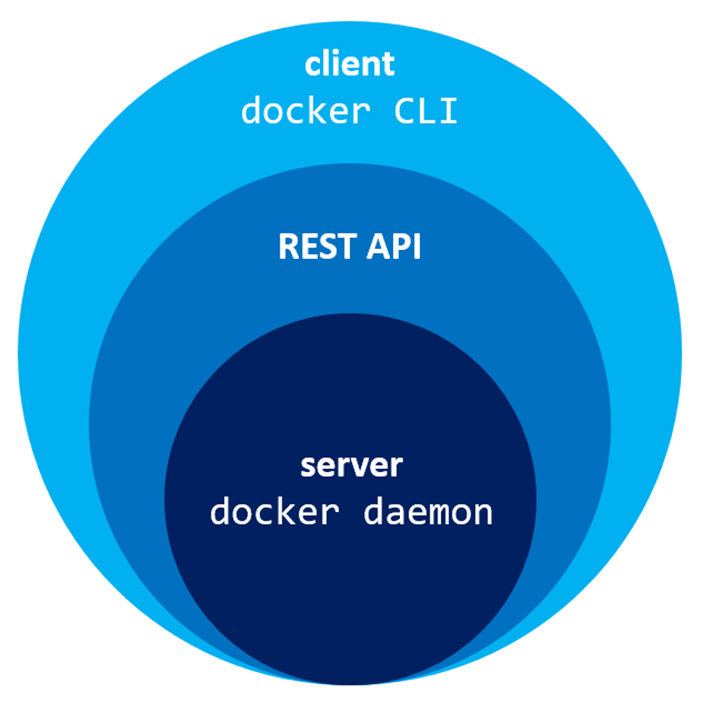
\includegraphics[width=10cm]{figuras/dockerStructure}}
\caption{Esquema de funcionamento de Docker}
\medskip
\small
\centerline{Fonte: \url{https://www.aquasec.com/wiki/display/containers/Docker+Containers}}
\label{dockerStructure}
\end{figure}

\begin{figure}
\centerline{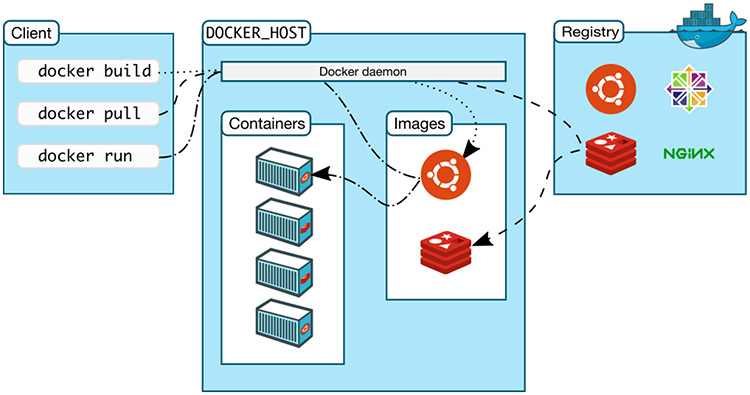
\includegraphics[width=15cm]{figuras/dockerStructure2}}
\caption{Modelo de despregamento de contedores en Docker}
\medskip
\small
\centerline{Fonte: \url{https://www.aquasec.com/wiki/display/containers/Docker+Containers}}
\label{dockerStructure2}
\end{figure}

\subsection{Seguridade}

Isto ten importantes implicacións de seguridade: exemplificando, se lanzamos Docker dende un servidor web para aprovisionar contedores a través dunha \gls{API}, deberiamos ser máis coidadosos do habitual coa comprobación de parámetros e outras medidas de seguridade para asegurar que un usuario malintencionado non poida pasar parámetros elaborados, facendo que o demo de Docker cree contedores arbitrarios.\\

Motivado por esta fenda de seguridade, o \textit{endpoint} da \gls{API} \gls{REST} de Docker trocou dun simple \textit{socket} \gls{TCP} a un \textit{socket} UNIX na súa versión 0.5.2, xa que o primeiro é considerado moito máis propenso a ataques \textit{cross-site}, se o demo se executa directamente na máquina anfitrioa e non está protexido por unha capa extra de virtualización mediante \gls{MV}s.

\section{Singularity}

\subsection{Funcionamento}

O primeiro que debemos comprender á hora de tratar con contedores Singularity é que esta tecnoloxía non parte da base de usuarios autorizados executando contedores autorizados, como moitas das tecnoloxías de contedorización existentes. Baixo ese enfoque, a tecnoloxía de contedorización debe ser controlada por un superusuario ou un usuario que fose autorizado para executar con permisos de tal. Alterando este punto de vista, o enfoque de Singularity parte da premisa de tratarse dunha tecnoloxía especializada para infraestruturas \gls{HPC}, onde existen moitos usuarios, pero case ningún deles é considerado fiábel, o que significa que é preciso abordar un paradigma distinto no que se deben soportar contedores non fiábel executados por usuarios non fiábeis. \cite{SingularitySecurity}\\

Para acadar este funcionamento, Singularity fai uso das seguintes ferramentas:

\begin{itemize}
    \item \textbf{SetUID:} este é o modelo predeterminado, posto que oferta a maior flexibilidade, mais tamén é o que máis riscos presenta dende a perspectiva da seguridade. Simplificando o seu funcionamento, un programa co SetUID activado por \textit{root}, poderá ser executado por outro usuario cos mesmos privilexios que \textit{root}. Por esta razón, os programas co SetUID activado son obxectivos habituais para os atacantes. Tendo isto en mente, Singularity foi desenvolvido atendendo á simplicidade e á lexibilidade, e só son outorgados privilexios de superusuario cando son estritamente precisos, quedando desactivados inmediatamente despois. Concretamente, as tarefas que precisan desta escalada de privilexios controlada son:
    \begin{itemize}
        \item Montaxe da imaxe no contedor Singularity.
        \item Creación dos espazos de nomes necesarios, coa axuda do \textit{kernel}.
        \item Compartición de directorios entre o contedor e a máquina anfitrioa, se así foi requirido.
    \end{itemize}
    Estes compoñentes co SetUID activado poden ser activados ou desactivados a pracer, tanto no momento da instalación como despois. Non obstante, perderemos as capacidades que estes outorgan.
    \item \textbf{Espazos de nomes:} Singularity admite a emprega de espazos de nomes de usuario de xeito nativo e poden executarse completamente sen privilexios dende a versión 2.2, mais cunhas funcionalidades moi limitadas. Por exemplo, só será posíbel empregar contedores baseados nun directorio. Ademais, posto que os espazos de nomes non son compatíbeis con todos os \textit{kernels} a súa empregabilidade pode variar.
\end{itemize}

\subsection{Fluxo de traballo}

O fluxo de funcionamento de Singularity normalmente implica que o usuario desenvolva nun dispositivo local ou nunha máquina virtual, no cal teña permisos de superusuario, e unha vez finalizado o desenvolvemento mova o contedor ao entorno de produción. En dito entorno non terá permisos de superusuario e non poderá facer cambios que requiran dos mesmos dentro do contedor, mais a solución é tan simple como volver ao entorno de desenvolvemento e facer os cambios pertinentes. Este modelo queda recollido na figura \ref{singularityWorkflow} dun xeito xeral, e na figura \ref{singularity-workflow} para o caso concreto do \gls{CESGA} sobre o \gls{FT2}.

\begin{figure}
\centerline{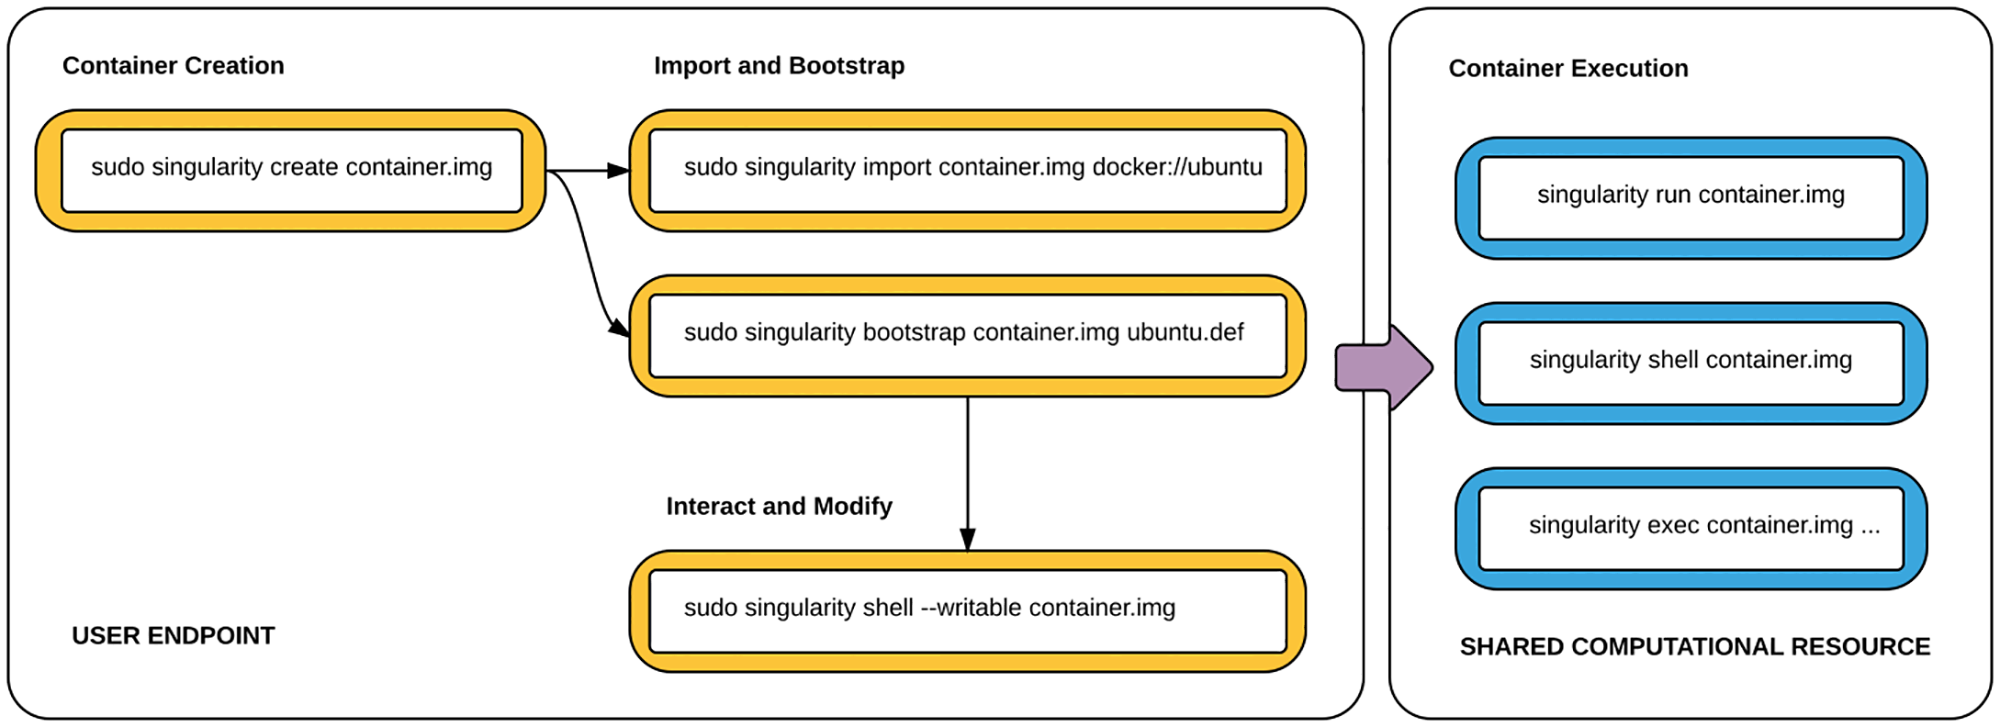
\includegraphics[width=15cm]{figuras/singularityWorkflow}}
\caption{Modelo de despregamento de contedores en Singularity}
\medskip
\small
\centerline{Fonte: \url{https://singularity.lbl.gov/}}
\label{singularityWorkflow}
\end{figure}

\begin{figure}
\centerline{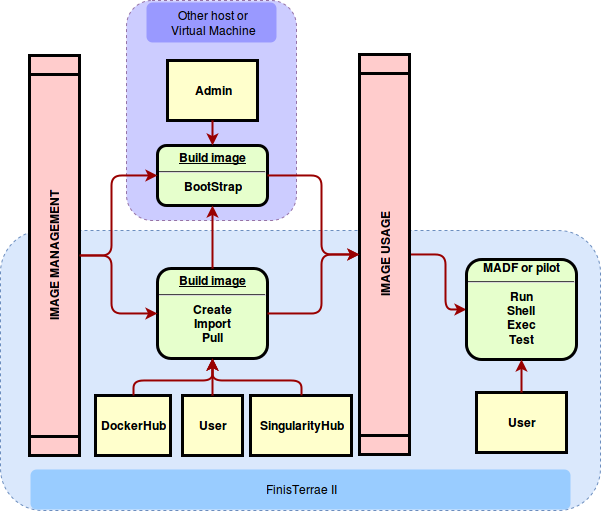
\includegraphics[width=15cm]{figuras/singularity-workflow.png}}
\caption{Modelo de despregamento de contedores en Singularity sobre \gls{FT2}}
\medskip
\small
\centerline{Fonte: \cite{MSO4SC}}
\label{singularity-workflow}
\end{figure}

\subsection{Seguridade}

O modelo de funcionamento de Singularity fai que se trate dunha ferramenta coa que dificilmente se poida abordar un ataque de escalada de privilexios, algo moi importante en entornos multiusuario. Isto é así porque o usuario a empregar unha vez lanzadas as execucións dos contedores é o mesmo usuario que está fóra do contedor. Se un usuario desexa ser superusuario dentro do contedor, primeiramente debe ser superusuario fóra do contedor.

\subsection{Compatibilidade con contedores Docker}

Posto que Docker estase a converter nun estándar na industria, resulta interesante poder ler e traballar con este tipo de contedores e aproveitar gran cantidade de traballo xa realizado. Así, Singularity soporta o tratamento de contedores Docker, sen ter que ter instalada dita tecnoloxía. Isto faise  mediante a emprega da \gls{API} do Docker Registry, unha interface \gls{REST} que da acceso aos manifestos das imaxes, cada un dous cales contén información sobre as capas das imaxes. Cada capa non é máis que un conxunto comprimido de carpetas e arquivos que poden ser extraídos directamente nunha imaxe Singularity. \cite{singularityScientificContainers}

\section{Udocker}
\label{introUdocker}

\subsection{Funcionamento}

Udocker é unha ferramenta que permite executar contedores simples de Docker nun espazo de usuario sen requirir de privilexios de superusuario, permitindo así a descarga e a execución de contedores Docker por usuarios non privilexiados en entornos Linux onde Docker non está dispoñíbel.\\

Pode ser empregado sen ningún tipo de privilexios no despregamento do servizo por parte do administrador do sistema, pudendo ser descargado e executado enteiramente polo usuario final.\\

Trátase dunha ferramenta sinxela escrita en Python, cun conxunto mínimo de dependencias que permiten que poida ser executado nun gran rango de entornos Linux, sen precisar tan sequera ter Docker instalado. O seu funcionamento baséase na emprega dun entorno tipo ``\textit{chroot}'', pero de xeito imitado, para non requirir privilexios en dito entorno. Para iso fai uso dunha serie de ferramentas e librarías coma poden ser:

\begin{itemize}
    \item PRoot
    \item Fakechroot
    \item runC
    \item Singularity
\end{itemize}

Este xeito de funcionar outorga unha serie de vantaxes. Por exemplo, o usuario final non terá que aprender unha nova ferramenta, pois de cara el compórtase exactamente como Docker (mesmos contedores, mesmos comandos, etc.). O usuario tampouco requirirá da axuda do administrador para despregar contedores nun equipo compartido, xa que non son precisos privilexios para a súa execución nin para a súa instalación; de feito, ao estar escrito en Python, nin tan sequera é preciso realizar o proceso de compilación, simplemente lanzar o script e executar. Destacar finalmente que foi testado sobre procesamento paralelo con aplicacións \gls{MPI} e \gls{GPGPU}. \cite{UdockerDoc}

\subsection{Limitacións}

Ao non existiren privilexios de superusuario involucrados, calquera operación que realmente precise ditos privilexios non será realizábel. Por exemplo, con Udocker é imposíbel realizar operacións como as seguintes:

\begin{itemize}
    \item Acceder a ficheiros e dispositivos protexidos pola máquina anfitrioa.
    \item Escoitar en portos TCP/IP privilexiados (rango embaixo do 1024).
    \item Montar sistemas de ficheiros.
    \item Emprega do comando \textit{su}.
    \item Cambio da hora do sistema.
    \item Operacións de rede complexas, tales como:
    \begin{itemize}
        \item Cambiar as táboas de enrutamento.
        \item Modificar regras nunha devasa.
        \item Tratamento con interfaces de rede.
    \end{itemize}
\end{itemize}

No caso de precisar realizar operacións como as anteriores, Udocker non é a tecnoloxía de contedorización adecuada e debemos optar por solucións alternativas. \cite{UdockerDoc}

\subsection{Seguridade}

O modelo de Udocker convérteo nunha solución relativamente segura, no sentido de que un atacante xamais poderá realizar un ataque de escalada de privilexios, ao non existir en ningún momento estes privilexios.\\

Non obstante, debido ás limitacións explicadas na sección anterior, Udocker non ofrece características avanzadas de illamento como poden ter outras tecnoloxías. Polo tanto, se o contido dos contedores non é fiábel, non debería ser executado baixo Udocker, xa que estes se executarán dentro do propio entorno do usuario. Os datos estarán suxeitos ás mesmas proteccións do sistemas que os outros arquivos propiedade do usuario.\\

Polo tanto, debido a esta falta de illamento, Udocker nunca debe ser executado por usuarios con privilexios.\\

\cleardoublepage
\chapter{Planificación e presupostos}
\minitoc
\clearpage

Este capítulo inclúe todos os aspectos relativos á xestión do proxecto, incluíndo a planificación temporal, a metodoloxía de desenvolvemento, a xestión de riscos e as estimación dos custos ou presupostos.

\section{Xestión de riscos}

\subsection{Introdución}

O actual proxecto implica certo carácter investigador, ao ter que procurar e recopilar posíbeis fallas na emprega de contedores, unha tecnoloxía que, á súa vez, aínda ten unha vida curta no eido da supercomputación.\\

Podemos concluír pois que o nivel de incerteza do proxecto resulta bastante elevado e, polo tanto, unha boa xestión de riscos resulta crucial para o adecuado desenvolvemento do mesmo. Cómpre detectar os riscos asociados ao proxecto para evitar o incumprimento de prazos ou sobrecustos innecesarios. É esencial a identificación destes posíbeis riscos, así como a aplicación de medidas para a súa prevención, miniaturización ou eliminación. Seguiranse os seguintes pasos:

\begin{enumerate}
    \item \textbf{Identificación de riscos:} detección de ameazas que poidan pór en perigo a viabilidade e desenvolvemento do proxecto.
    
    \item \textbf{Análise e clasificación:} unha vez detectadas as ameazas existentes, serán avaliadas individualmente para determinar se supón un risco para o proxecto. Cada risco terá asociados unha probabilidade e impacto, grazas aos cales poderemos realizar unha planificación fronte a estes. De ter asociados un impacto e/ou probabilidade de suceso moi baixos, descartaranse do plan de resposta.
    
    \item \textbf{Planificación:} clasificados os riscos, serán explicadas as medidas de prevención, miniaturización ou continxencia a aplicar.
    
    \item \textbf{Seguimento:} realizados os pasos anteriores, cómpre realizar un seguimento dos riscos ao longo do proxecto para comprobar a súa evolución e posíbel materialización, co fin de dar resposta no menor tempo posíbel.
\end{enumerate}

Para comprender adecuadamente a continuación desta sección, cómpre entender unha serie de conceptos: os riscos son a probabilidade de que as ameazas actúen sobre os activos, causando danos ou perdas. Os activos son os compoñentes ou funcionalidades susceptíbeis de seren atacados, deliberada ou accidentalmente, con consecuencias para o organismo, entidade ou sistema. As vulnerabilidades son as debilidades ou falla de control que permitiría ou facilitaría que unha ameaza actúe contra un activo. Unha ameaza é unha circunstancia ou evento que pode explotar, intencionadamente ou non, unha vulnerabilidade específica. O impacto é o dano causado nun activo como resultado da explotación dunha vulnerabilidade por unha ameaza.

\subsection{Medidores dos riscos}

Os medidores dos riscos serán os seguintes:

\begin{itemize}
    \item \textbf{Probabilidade} de suceso dun risco:
    \begin{itemize}
        \item \textbf{Baixa:} menos de 25\% de posibilidades de suceso.
        \item \textbf{Media:} entre 25\% e 75\% de posibilidades de suceso.
        \item \textbf{Alta:} máis de 75\% de posibilidades de suceso.
    \end{itemize}
    
    \item \textbf{Impacto} en tempo, esforzo ou custo do suceso dun risco:
    \begin{itemize}
        \item \textbf{Insignificante:} a manifestación do risco terá unha repercusión mínima no desenvolvemento do proxecto.
        \item \textbf{Tolerábel:} a manifestación do risco provocará atrasos na realización das tarefas asociadas ao proxecto, mais será posíbel realizar a entrega do proxecto nos prazos establecidos.
        \item \textbf{Serio:} a manifestación do risco provocará que a entrega do TFG se realice noutra convocatoria.
        \item \textbf{Catastrófico:} a manifestación do risco provocará que non sexa posíbel realizar a entrega do proxecto no prazo dun ano. Tal feito implicaría refacer o TFG enteiramente.
    \end{itemize}
    
    \item \textbf{Nivel de exposición:} combinación dos anteriores valores de probabilidade e impacto, converténdoos nunha medida tanxíbel. Para isto é preciso asociar os anteriores medidores con valores numéricos. A valoración da probabilidade pode ser consultada na táboa \ref{valoracionProbabilidade} e valoración do impacto, na táboa \ref{valoracionImpacto}.
    
\begin{table}[]
\centering
\caption{Valoración da probabilidade}
\label{valoracionProbabilidade}
\begin{tabular}{|c|c|}
\hline
\textbf{Probabilidade} & \textbf{Valor numérico asociado} \\ \hline
Baixa & 0.2 \\ \hline
Media & 0.5 \\ \hline
Alta & 0.8 \\ \hline
\end{tabular}
\end{table}

\begin{table}[]
\centering
\caption{Valoración do impacto}
\label{valoracionImpacto}
\begin{tabular}{|c|c|}
\hline
\textbf{Impacto} & \textbf{Valor numérico asociado} \\ \hline
Insignificante & 0.1 \\ \hline
Tolerábel & 0.4 \\ \hline
Serio & 0.6 \\ \hline
Catastrófico & 0.9 \\ \hline
\end{tabular}
\end{table}

Establecidas estas valoracións, é posíbel obter o nivel de exposición, resultado do produto dos dous valores anteriormente definidos, reflectido na táboa \ref{nivelExposicionRisco}. Serán definidos os seguintes tipos de exposición segundo os valores obtidos en dita táboa:

\begin{itemize}
    \item \textbf{Baixa:} valor da exposición comprendido entre 0 e 0.15.
    \item \textbf{Media:} valor da exposición comprendido entre 0.16 e 0.4.
    \item \textbf{Alta:} valor da exposición estritamente maior que 0.4.
\end{itemize}


\begin{table}[]
\centering
\caption{Nivel de exposición ao risco}
\label{nivelExposicionRisco}
\resizebox{\textwidth}{!}{%
\begin{tabular}{|c|c|c|c|c|c|}
\hline
\multicolumn{2}{|c|}{\multirow{2}{*}{}} & \multicolumn{4}{c|}{Impacto} \\ \cline{3-6} 
\multicolumn{2}{|c|}{} & Insignificante (0.1) & Tolerábel (0.4) & Serio (0.6) & Catastrófico (0.9) \\ \hline
\multirow{3}{*}{Probabilidade} & Baixa (0.2) & 0.02 & 0.08 & 0.12 & 0.18 \\ \cline{2-6} 
 & Media (0.5) & 0.05 & 0.2 & 0.3 & 0.45 \\ \cline{2-6} 
 & Alta (0.8) & 0.08 & 0.32 & 0.48 & 0.72 \\ \hline
\end{tabular}
}
\end{table}

\end{itemize}

\subsection{Tipos de riscos}

Para a clasificación dos riscos seguirase a categorización de Sommerville \cite{Sommerville}, segundo a cal existen tres tipos de riscos:

\begin{enumerate}
    \item \textbf{De proxecto:} afectan á programación temporal ou aos recursos.
    \item \textbf{De produto:} afectan á calidade ou desempeño do produto.
    \item \textbf{De negocio:} afectan á organización responsábel do desenvolvemento.
\end{enumerate}

\subsection{Tipos de estratexias a seguir}

Unha vez identificados os posíbeis riscos que poidan afectar ao proxecto, cómpre realizar unha análise de cada un deles, para poder realizar a súa categorización en base á súa relevancia. Contémplanse varios métodos para combater un risco potencial:

\begin{itemize}
    \item \textbf{Prevención:} baséase en reducir a probabilidade de que un risco se materialice.
    \item \textbf{Miniaturización:} baséase en reducir o impacto xerado polo risco.
    \item \textbf{Aceptación:} baséase en asumir o impacto asociado ao risco e as súas consecuencias.
    \item \textbf{Continxencia:} baséase na aplicación dun plan de continxencia no que aparezan accións a realizar en caso de que aconteza un risco.
    \item \textbf{Transferencia:} baséase no traspaso do risco a outra entidade que o xestione por nós.
\end{itemize}

\subsection{Identificación de ameazas}

\begin{table}[H]
\caption{Ameaza A1}
\label{A1}
\begin{tabularx}{\textwidth}{|l|X|}
\hline
\textbf{Identificador} & A1 \\ \hline
\textbf{Nome} & Perda do repositorio local. \\ \hline
\textbf{Descrición} & O repositorio gardado no equipo de traballo pérdese por mor dun fallo no disco duro. Isto provoca que se perda a última versión dos elementos da configuración. \\ \hline
\end{tabularx}
\end{table}

\begin{table}[H]
\caption{Ameaza A2}
\label{A2}
\begin{tabularx}{\textwidth}{|l|X|}
\hline
\textbf{Identificador} & A2 \\ \hline
\textbf{Nome} & Atraso na realización dun fito. \\ \hline
\textbf{Descrición} & Un fito reflectido na planificación inicial do proxecto, é dicir, no anteproxecto, non é acadado no prazo previsto debido a improvisos na realización do traballo. \\ \hline
\end{tabularx}
\end{table}

\begin{table}[H]
\caption{Ameaza A3}
\label{A3}
\begin{tabularx}{\textwidth}{|l|X|}
\hline
\textbf{Identificador} & A3 \\ \hline
\textbf{Nome} & Elementos da configuración non identificados. \\ \hline
\textbf{Descrición} & Son ignorados algúns elementos da configuración á hora de realizar a identificación dos mesmos, polo que non serán xestionados no proceso de xestión da configuración a empregar no proxecto. \\ \hline
\end{tabularx}
\end{table}

\begin{table}[H]
\caption{Ameaza A4}
\label{A4}
\begin{tabularx}{\textwidth}{|l|X|}
\hline
\textbf{Identificador} & A4 \\ \hline
\textbf{Nome} & Identificación de elementos da configuración innecesarios. \\ \hline
\textbf{Descrición} & Son detectados elementos da configuración que deben ser xestionados, mais que finalmente non resultan relevantes para a execución do proxecto, o que provoca atrasos á hora de realizar a xestión da configuración do proxecto. \\ \hline
\end{tabularx}
\end{table}

\begin{table}[H]
\caption{Ameaza A5}
\label{A5}
\begin{tabularx}{\textwidth}{|l|X|}
\hline
\textbf{Identificador} & A5 \\ \hline
\textbf{Nome} & Definición dun proceso da xestión da configuración ineficaz e/ou incorrecto. \\ \hline
\textbf{Descrición} & Á hora de executar o proceso de configuración, obsérvanse erros que dificultan a consecución dos obxectivos precisos para a realización do proxecto. \\ \hline
\end{tabularx}
\end{table}

\begin{table}[H]
\caption{Ameaza A6}
\label{A6}
\begin{tabularx}{\textwidth}{|l|X|}
\hline
\textbf{Identificador} & A6 \\ \hline
\textbf{Nome} & Non é definido un proceso de xestión da configuración. \\ \hline
\textbf{Descrición} & Non é definido un proceso de xestión da configuración na fase inicial do proxecto. \\ \hline
\end{tabularx}
\end{table}

\begin{table}[H]
\caption{Ameaza A7}
\label{A7}
\begin{tabularx}{\textwidth}{|l|X|}
\hline
\textbf{Identificador} & A7 \\ \hline
\textbf{Nome} & Proceso de xestión da configuración excesivamente burocrático. \\ \hline
\textbf{Descrición} & O proceso de xestión da configuración elixido ou deseñado require dunha cantidade de documentación moi superior á precisa. Isto podería chegar a provocar atrasos nos fitos do proxecto, pois é destinada unha cantidade de tempo significativa no tratamento destes documentos. \\ \hline
\end{tabularx}
\end{table}

\begin{table}[H]
\caption{Ameaza A8}
\label{A8}
\begin{tabularx}{\textwidth}{|l|X|}
\hline
\textbf{Identificador} & A8 \\ \hline
\textbf{Nome} & Ausencia de copia de seguridade do repositorio. \\ \hline
\textbf{Descrición} & O repositorio do proxecto está almacenado nunha única localización e dita localización perde os datos correspondentes ao proxecto. \\ \hline
\end{tabularx}
\end{table}

\begin{table}[H]
\caption{Ameaza A9}
\label{A9}
\begin{tabularx}{\textwidth}{|l|X|}
\hline
\textbf{Identificador} & A9 \\ \hline
\textbf{Nome} & Entrega dunha versión incorrecta. \\ \hline
\textbf{Descrición} & Á hora de realizar a entrega final prodúcese unha confusión na versión a entregar, o que provoca que se entregue unha versión anterior á final. \\ \hline
\end{tabularx}
\end{table}

\begin{table}[H]
\caption{Ameaza A10}
\label{A10}
\begin{tabularx}{\textwidth}{|l|X|}
\hline
\textbf{Identificador} & A10 \\ \hline
\textbf{Nome} & Incumprimento das horas de traballo. \\ \hline
\textbf{Descrición} & O proxecto débese axustar a unhas horas establecidas, correspondentes ao número de créditos asinados á materia do Traballo de Fin de Grao. No caso de incumprir a estimación temporal debe ser exposta unha razón. \\ \hline
\end{tabularx}
\end{table}

\begin{table}[H]
\caption{Ameaza A11}
\label{A11}
\begin{tabularx}{\textwidth}{|l|X|}
\hline
\textbf{Identificador} & A11 \\ \hline
\textbf{Nome} & Actualizacións do repositorio demasiado espazadas no tempo.  \\ \hline
\textbf{Descrición} & O tempo entre as diferentes actualizacións no repositorio é excesivamente longo, o que pode provocar que de querer volver a unha versión antiga, pérdanse cambios que poidan ser considerados de relevancia. \\ \hline
\end{tabularx}
\end{table}

\begin{table}[H]
\caption{Ameaza A12}
\label{A12}
\begin{tabularx}{\textwidth}{|l|X|}
\hline
\textbf{Identificador} & A12 \\ \hline
\textbf{Nome} & Equipo de traballo avariado. \\ \hline
\textbf{Descrición} & O equipo de traballo co que conta o estudante fica avariado, impedindo a realización do proxecto. \\ \hline
\end{tabularx}
\end{table}

\begin{table}[H]
\caption{Ameaza A13}
\label{A13}
\begin{tabularx}{\textwidth}{|l|X|}
\hline
\textbf{Identificador} & A13 \\ \hline
\textbf{Nome} & Roubo de material \\ \hline
\textbf{Descrición} & Perda de material (non dixital) por mor dun roubo no lugar de traballo. \\ \hline
\end{tabularx}
\end{table}

\begin{table}[H]
\caption{Ameaza A14}
\label{A14}
\begin{tabularx}{\textwidth}{|l|X|}
\hline
\textbf{Identificador} & A14 \\ \hline
\textbf{Nome} & Caída dun dos portais de contedores a empregar. \\ \hline
\textbf{Descrición} & Un dos portais de onde se descargan as imaxes dos contedores a empregar para o desenvolvemento do proxecto cae, quedando inoperante e impedindo a obtención de imaxes importantes para o traballo. \\ \hline
\end{tabularx}
\end{table}

\begin{table}[H]
\caption{Ameaza A15}
\label{A15}
\begin{tabularx}{\textwidth}{|l|X|}
\hline
\textbf{Identificador} & A15 \\ \hline
\textbf{Nome} & Caída dos entornos de pre-produción ou produción. \\ \hline
\textbf{Descrición} & Os entornos de pre-predución (computación na nube) ou produción do \gls{CESGA} caen, impedindo a realización das probas precisas para o desenvolvemento dou proxecto, ou ocasionando a perda de información importante. \\ \hline
\end{tabularx}
\end{table}

\subsection{Identificación de activos}

\begin{enumerate}[{ACT}1: ]
    \item Equipo de traballo.
    \item Memoria do proxecto.
    \item Repositorio.
    \item Proceso de xestión da configuración.
    \item Contedores sobre os que realizar as probas.
    \item Material de traballo non dixital: apuntamentos, libros, etc.
    \item Infraestrutura do \gls{CESGA}.
    \item Imaxes e diagramas.
    \item \textit{Scripts}.
\end{enumerate}

\subsection{Análise de riscos}

Como xa foi visto, os riscos son a probabilidade de que as ameazas actúen sobre os activos, causando danos ou perdas, polo que cada risco estará relacionado cunha das ameazas estudadas previamente. Está correlación virá indicada polo seu número do identificador, que será o mesmo para a ameaza e o risco.

\begin{table}[H]
\centering
\caption{Risco R1}
\label{R1}
\begin{tabularx}{\textwidth}{|l|l|l|l|}
\hline
\textbf{Identificador} & R1 & \textbf{Tipo de risco} & De produto \\ \hline
\textbf{Probabilidade} & Baixa & \textbf{Impacto} & Tolerábel \\ \hline
\textbf{Exposición} & Baixa & \textbf{Activos afectados} & ACT1, ACT2, ACT8, ACT9 \\ \hline
\multicolumn{1}{|l|}{\textbf{Tratamento}} & \multicolumn{3}{X|}{\tabitem \textbf{Aceptación:} enténdese que os últimos datos xa están perdidos, ao non ter realizado unha actualización do repositorio remoto. Ao ter unha exposición baixa podemos aceptar este risco sen moito problema, soamente habería que repetir os últimos avances.} \\ \hline
\multicolumn{1}{|l|}{\textbf{Indicadores}} & \multicolumn{3}{X|}{O sistema non permite acceder aos últimos cambios realizados en disco no proxecto.} \\ \hline
\end{tabularx}
\end{table}

\begin{table}[H]
\centering
\caption{Risco R2}
\label{R3}
\begin{tabularx}{\textwidth}{|l|l|l|l|}
\hline
\textbf{Identificador} & R2 & \textbf{Tipo de risco} & De proxecto \\ \hline
\textbf{Probabilidade} & Media & \textbf{Impacto} & Tolerábel \\ \hline
\textbf{Exposición} & Media & \textbf{Activos afectados} & ACT2 \\ \hline
\multicolumn{1}{|l|}{\textbf{Tratamento}} & \multicolumn{3}{X|}{\tabitem \textbf{Prevención:} realización dunha boa planificación.


\tabitem \textbf{Miniaturización:} incluír tarefas con pouca relevancia nunha sección de tarefas excluídas.} \\ \hline
\multicolumn{1}{|l|}{\textbf{Indicadores}} & \multicolumn{3}{X|}{Algunha das tarefas a realizar, definidas no anteproxecto, superou por un prazo superior a 2 días o seu tempo previsto de execución.} \\ \hline
\end{tabularx}
\end{table}

\begin{table}[H]
\centering
\caption{Risco R3}
\label{R3}
\begin{tabularx}{\textwidth}{|l|l|l|l|}
\hline
\textbf{Identificador} & R3 & \textbf{Tipo de risco} & De produto \\ \hline
\textbf{Probabilidade} & Media & \textbf{Impacto} & Tolerábel \\ \hline
\textbf{Exposición} & Media & \textbf{Activos afectados} & ACT3, ACT4 \\ \hline
\multicolumn{1}{|l|}{\textbf{Tratamento}} & \multicolumn{3}{X|}{\tabitem \textbf{Prevención:} identificación adecuada dos elementos da configuración e realización dunha xestión da configuración simple e eficiente.


\tabitem \textbf{Miniaturización:} detectado o problema, realizar modificacións na xestión da configuración para incluír o novo elemento non identificado previamente. Posto que o equipo de traballo é dunha soa persoa, non debería haber problema por realizar cambios pequenos e xustificados na xestión da configuración.} \\ \hline
\multicolumn{1}{|l|}{\textbf{Indicadores}} & \multicolumn{3}{X|}{Cando o proxecto avanza, obsérvase que hai elementos que non están sendo contemplados na xestión da configuración, ao non ter sido considerados elementos da configuración en si.} \\ \hline
\end{tabularx}
\end{table}

\begin{table}[H]
\centering
\caption{Risco R4}
\label{R4}
\begin{tabularx}{\textwidth}{|l|l|l|l|}
\hline
\textbf{Identificador} & R4 & \textbf{Tipo de risco} & De produto \\ \hline
\textbf{Probabilidade} & Media & \textbf{Impacto} & Tolerábel \\ \hline
\textbf{Exposición} & Media & \textbf{Activos afectados} & ACT3, ACT4 \\ \hline
\multicolumn{1}{|l|}{\textbf{Tratamento}} & \multicolumn{3}{X|}{\tabitem \textbf{Prevención:} identificación adecuada dos elementos da configuración e realización dunha xestión da configuración simple e eficiente.


\tabitem \textbf{Miniaturización:} detectado o problema, realizar modificacións na xestión da configuración para excluír os elementos sobrantes. Posto que o equipo de traballo é dunha soa persoa, non debería haber problema por realizar cambios pequenos e xustificados na xestión da configuración.} \\ \hline
\multicolumn{1}{|l|}{\textbf{Indicadores}} & \multicolumn{3}{X|}{Cando o proxecto avanza, obsérvase que hai elementos que non son precisos para o correcto desenvolvemento do proxecto, polo que o seu control implica unha perda de tempo innecesaria.} \\ \hline
\end{tabularx}
\end{table}


\begin{table}[H]
\centering
\caption{Risco R5}
\label{R5}
\begin{tabularx}{\textwidth}{|l|l|l|l|}
\hline
\textbf{Identificador} & R5 & \textbf{Tipo de risco} & De produto \\ \hline
\textbf{Probabilidade} & Media & \textbf{Impacto} & Tolerábel \\ \hline
\textbf{Exposición} & Media & \textbf{Activos afectados} & ACT3, ACT4 \\ \hline
\multicolumn{1}{|l|}{\textbf{Tratamento}} & \multicolumn{3}{X|}{\tabitem \textbf{Prevención:} deseño dunha xestión da configuración adecuada ao proxecto e que resulte eficaz e eficiente.


\tabitem \textbf{Miniaturización:} detectado o problema, realizar modificacións na xestión da configuración para que esta se adapte correctamente ao proxecto. Posto que o equipo de traballo é dunha soa persoa, non debería haber problema por realizar cambios pequenos e xustificados na xestión da configuración.} \\ \hline
\multicolumn{1}{|l|}{\textbf{Indicadores}} & \multicolumn{3}{X|}{Cando o proxecto avanza, obsérvanse serios problemas para levar a cabo a xestión da configuración (por exemplo, modelos inservíbeis ou incompletos).} \\ \hline
\end{tabularx}
\end{table}


\begin{table}[H]
\centering
\caption{Risco R6}
\label{R6}
\begin{tabularx}{\textwidth}{|l|l|l|l|}
\hline
\textbf{Identificador} & R6 & \textbf{Tipo de risco} & De produto \\ \hline
\textbf{Probabilidade} & Baixa & \textbf{Impacto} & Serio \\ \hline
\textbf{Exposición} & Baixa & \textbf{Activos afectados} & ACT3, ACT4 \\ \hline
\multicolumn{1}{|l|}{\textbf{Tratamento}} & \multicolumn{3}{X|}{\tabitem \textbf{Prevención:} deseño dunha xestión da configuración adecuada ao inicio do proxecto.} \\ \hline
\multicolumn{1}{|l|}{\textbf{Indicadores}} & \multicolumn{3}{X|}{Non é posíbel realizar unha xestión da configuración e non están quedando almacenados os diferentes cambios no proxecto en ningún momento.} \\ \hline
\end{tabularx}
\end{table}


\begin{table}[H]
\centering
\caption{Risco R7}
\label{R7}
\begin{tabularx}{\textwidth}{|l|l|l|l|}
\hline
\textbf{Identificador} & R7 & \textbf{Tipo de risco} & De produto \\ \hline
\textbf{Probabilidade} & Media & \textbf{Impacto} & Tolerábel \\ \hline
\textbf{Exposición} & Media & \textbf{Activos afectados} & ACT3, ACT4 \\ \hline
\multicolumn{1}{|l|}{\textbf{Tratamento}} & \multicolumn{3}{X|}{\tabitem \textbf{Prevención:} deseño dunha xestión da configuración adecuada ao proxecto e que resulte eficaz e eficiente.


\tabitem \textbf{Miniaturización:} detectado o problema, realizar modificacións na xestión da configuración para que esta se adapte correctamente ao proxecto. Posto que o equipo de traballo é dunha soa persoa, non debería haber problema por realizar cambios pequenos e xustificados na xestión da configuración.} \\ \hline
\multicolumn{1}{|l|}{\textbf{Indicadores}} & \multicolumn{3}{X|}{Cando o proxecto avanza, detéctase unha perda de tempo excesiva no tratamento da xestión da configuración.} \\ \hline
\end{tabularx}
\end{table}


\begin{table}[H]
\centering
\caption{Risco R8}
\label{R8}
\begin{tabularx}{\textwidth}{|l|l|l|l|}
\hline
\textbf{Identificador} & R8 & \textbf{Tipo de risco} & De proxecto \\ \hline
\textbf{Probabilidade} & Baixa & \textbf{Impacto} & Catastrófico \\ \hline
\textbf{Exposición} & Media & \textbf{Activos afectados} & ACT2, ACT3, ACT8, ACT9 \\ \hline
\multicolumn{1}{|l|}{\textbf{Tratamento}} & \multicolumn{3}{X|}{\tabitem \textbf{Prevención:} establecer o proceso de xestión da configuración de tal forma que o repositorio de traballo estea almacenado en múltiples localizacións, preferibelmente afastadas no espazo.} \\ \hline
\multicolumn{1}{|l|}{\textbf{Indicadores}} & \multicolumn{3}{X|}{Soamente existe unha copia do proxecto, non sendo posíbel acceder a outras copias de seguridade.} \\ \hline
\end{tabularx}
\end{table}

\begin{table}[H]
\centering
\caption{Risco R9}
\label{R9}
\begin{tabularx}{\textwidth}{|l|l|l|l|}
\hline
\textbf{Identificador} & R9 & \textbf{Tipo de risco} & De produto \\ \hline
\textbf{Probabilidade} & Baixa & \textbf{Impacto} & Serio \\ \hline
\textbf{Exposición} & Baixa & \textbf{Activos afectados} & ACT2, ACT8, ACT9 \\ \hline
\multicolumn{1}{|l|}{\textbf{Tratamento}} & \multicolumn{3}{X|}{\tabitem \textbf{Prevención:} revisión ao menos dúas veces de que a versión a entregar concorda coas últimas modificacións realizadas no proxecto.} \\ \hline
\multicolumn{1}{|l|}{\textbf{Indicadores}} & \multicolumn{3}{X|}{O proxecto obtido pola comisión de traballos de fin de grao non é o mesmo que a última versión que posúe o autor.} \\ \hline
\end{tabularx}
\end{table}

\begin{table}[H]
\centering
\caption{Risco R10}
\label{R10}
\begin{tabularx}{\textwidth}{|l|l|l|l|}
\hline
\textbf{Identificador} & R10 & \textbf{Tipo de risco} & De proxecto \\ \hline
\textbf{Probabilidade} & Alta & \textbf{Impacto} & Serio \\ \hline
\textbf{Exposición} & Alta & \textbf{Activos afectados} & ACT2 \\ \hline
\multicolumn{1}{|l|}{\textbf{Tratamento}} & \multicolumn{3}{X|}{\tabitem \textbf{Prevención:} realización dunha boa planificación temporal e seguimento dunha metodoloxía áxil para evitar os riscos asociados á incerteza do proxecto.} \\ \hline
\multicolumn{1}{|l|}{\textbf{Indicadores}} & \multicolumn{3}{X|}{\tabitem As tarefas definidas no anteproxecto están levando máis tempo do esperado.

\tabitem Non se está seguindo ningunha metodoloxía de traballo áxil.} \\ \hline
\end{tabularx}
\end{table}

\begin{table}[H]
\centering
\caption{Risco R11}
\label{R11}
\begin{tabularx}{\textwidth}{|l|l|l|l|}
\hline
\textbf{Identificador} & R11 & \textbf{Tipo de risco} & De proxecto \\ \hline
\textbf{Probabilidade} & Media & \textbf{Impacto} & Tolerábel \\ \hline
\textbf{Exposición} & Media & \textbf{Activos afectados} & \scriptsize{ACT2, ACT3, ACT4, ACT8, ACT9} \\ \hline
\multicolumn{1}{|l|}{\textbf{Tratamento}} & \multicolumn{3}{X|}{\tabitem \textbf{Prevención:} establecer na xestión da configuración un procedemento de xestión de cambios en intres reducidos de tempo.} \\ \hline
\multicolumn{1}{|l|}{\textbf{Indicadores}} & \multicolumn{3}{X|}{Cando se quere retroceder a unha versión anterior empregando a xestión da configuración, moitos datos son perdidos, que ben poderían estar diferenciados en \textit{commits} distintos para evitar a súa perda.} \\ \hline
\end{tabularx}
\end{table}

\begin{table}[H]
\centering
\caption{Risco R12}
\label{R12}
\begin{tabularx}{\textwidth}{|l|l|l|l|}
\hline
\textbf{Identificador} & R12 & \textbf{Tipo de risco} & De negocio \\ \hline
\textbf{Probabilidade} & Baixa & \textbf{Impacto} & Catastrófico \\ \hline
\textbf{Exposición} & Media & \textbf{Activos afectados} & ACT1 \\ \hline
\multicolumn{1}{|l|}{\textbf{Tratamento}} & \multicolumn{3}{X|}{\tabitem \textbf{Prevención:} poder contar cun equipo de reposto para poder continuar co traballo nun período inferior a 12 horas.} \\ \hline
\multicolumn{1}{|l|}{\textbf{Indicadores}} & \multicolumn{3}{X|}{Non é posíbel traballar co equipo de traballo ou facelo de xeito adecuado para o desenvolvemento do proxecto.} \\ \hline
\end{tabularx}
\end{table}

\begin{table}[H]
\centering
\caption{Risco R13}
\label{R13}
\begin{tabularx}{\textwidth}{|l|l|l|l|}
\hline
\textbf{Identificador} & R13 & \textbf{Tipo de risco} & De negocio \\ \hline
\textbf{Probabilidade} & Baixa & \textbf{Impacto} & Serio \\ \hline
\textbf{Exposición} & Baixa & \textbf{Activos afectados} & ACT1, ACT6, ACT7 \\ \hline
\multicolumn{1}{|l|}{\textbf{Tratamento}} & \multicolumn{3}{X|}{\tabitem \textbf{Transferencia:} o \gls{CESGA} dispón de medidas físicas de seguridade para evitar este tipo de sucesos. A zona de traballo non é accesíbel sen previa identificación e existe seguridade mediante gravación do centro.} \\ \hline
\multicolumn{1}{|l|}{\textbf{Indicadores}} & \multicolumn{3}{X|}{Desaparece parte ou a totalidade dos materiais físicos de traballo.} \\ \hline
\end{tabularx}
\end{table}

\begin{table}[H]
\centering
\caption{Risco R14}
\label{R14}
\begin{tabularx}{\textwidth}{|l|l|l|l|}
\hline
\textbf{Identificador} & R14 & \textbf{Tipo de risco} & De proxecto \\ \hline
\textbf{Probabilidade} & Baixa & \textbf{Impacto} & Serio \\ \hline
\textbf{Exposición} & Baixa & \textbf{Activos afectados} & ACT5 \\ \hline
\multicolumn{1}{|l|}{\textbf{Tratamento}} & \multicolumn{3}{X|}{\tabitem \textbf{Aceptación:} posto que se trata dun servizo completamente externo, non é posíbel aplicar moitas medidas. Tentarase traballar coas imaxes xa almacenadas no equipo local, mais no caso de querer facer probas directamente co portal non haberá nada que facer, agás agardar á súa recuperación.} \\ \hline
\multicolumn{1}{|l|}{\textbf{Indicadores}} & \multicolumn{3}{X|}{Resulta imposíbel acceder a algún dos portais de imaxes de contedores cos que se traballa ao longo do proxecto (obtención de erro 404 ou similar).} \\ \hline
\end{tabularx}
\end{table}

\begin{table}[H]
\centering
\caption{Risco R15}
\label{R15}
\begin{tabularx}{\textwidth}{|l|l|l|l|}
\hline
\textbf{Identificador} & R15 & \textbf{Tipo de risco} & De negocio \\ \hline
\textbf{Probabilidade} & Baixa & \textbf{Impacto} & Catastrófico \\ \hline
\textbf{Exposición} & Media & \textbf{Activos afectados} & ACT7 \\ \hline
\multicolumn{1}{|l|}{\textbf{Tratamento}} & \multicolumn{3}{X|}{\tabitem \textbf{Transferencia:} o \gls{CESGA} dispón de medidas para minimizar o impacto en caso de que este tipo de risco se materialice. Por exemplo, existen copias de seguridade programadas para evitar a perda da totalidade do traballo. Tamén existen medidas de prevención como un xerador de electricidade ou unha múltiple conexión coa rede externa mediante diversos servizos para asegurar o continuo funcionamento do sistema.} \\ \hline
\multicolumn{1}{|l|}{\textbf{Indicadores}} & \multicolumn{3}{X|}{Resulta imposíbel acceder aos entornos de pre-produción ou produción.} \\ \hline
\end{tabularx}
\end{table}

\subsection{Seguimento dos riscos}

Realizados os pasos de identificación, análise, clasificación e planificación, só queda realizar un seguimento dos riscos ao longo da vida do proxecto. Este seguimento seguiuse rigorosamente, feito que permitiu a detección da materialización dun dos riscos identificados.

\subsubsection{Seguimento do risco R14}

Materializouse o risco R14, a caída dun dos portais de imaxes de contedores, o Docker Hub. As medidas a tomar neste caso eran simplemente de aceptación, ao non ter control sobre servizos externos. Afortunadamente, este risco materializouse o 24 de xuño do 2018, cando todas as probas relacionadas con este portal xa estaban satisfactoriamente completadas. De todos os xeitos, a caída foi solucionada axiña polos responsábeis do portal, polo que non tería moito impacto no desenvolvemento do proxecto de ter ocorrido noutro momento no que si fixera falla a emprega deste portal (simplemente a agarda dunhas horas).\\

A figura \ref{caidaAgora} amosa a caída ou falla dalgúns dos sistemas do Docker Hub o día 24 de xuño de 2018, grazas a ferramenta de seguimento que Docker dispón ao público, o \textit{Docker System Status}\footnote{\url{https://status.docker.com/}}. A figura \ref{caidaPasada} amosa os problemas presentados no sistema dende unha ollada histórica, superado xa o incidente.\\

\begin{figure}
\centerline{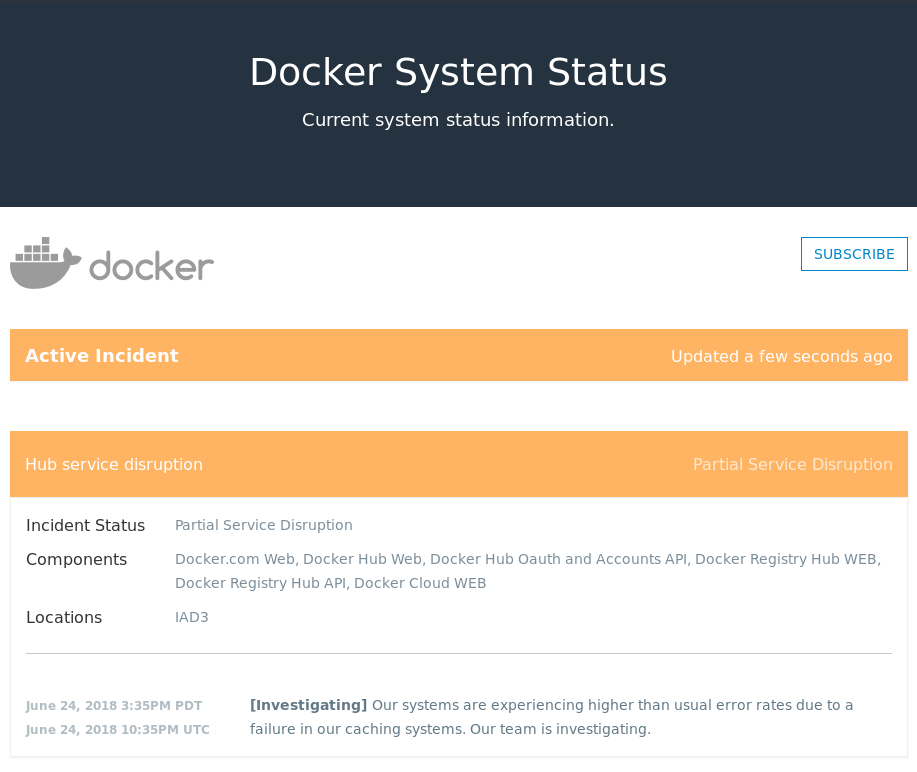
\includegraphics[width=15cm]{figuras/caidaAgora.png}}
\caption{Caída dos sistemas do Docker Hub}
\label{caidaAgora}
\end{figure}

\begin{figure}
\centerline{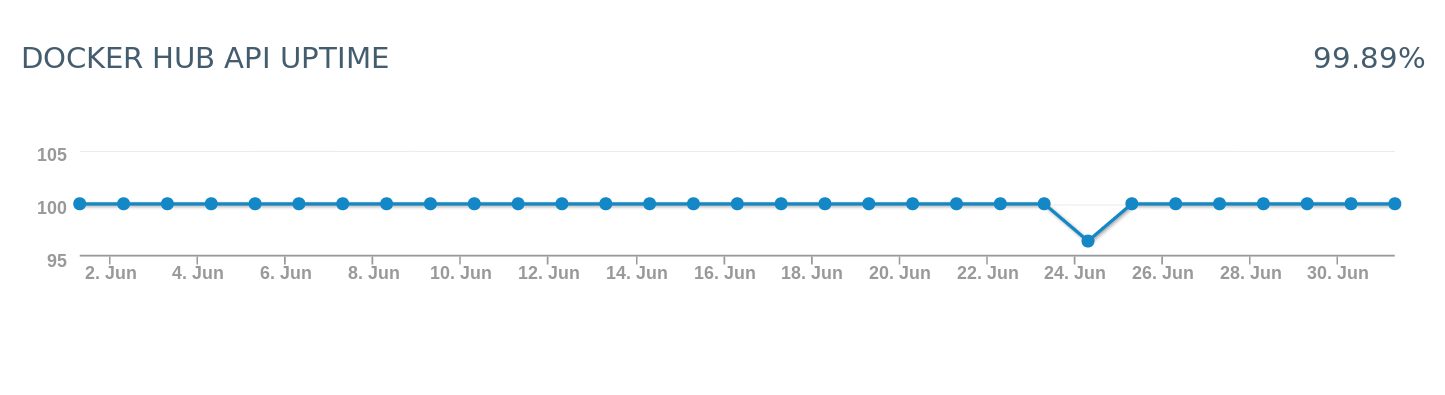
\includegraphics[width=15cm]{figuras/caidaPasada.png}}
\caption{Histórico do estado de saúde dos sistemas do Docker Hub}
\label{caidaPasada}
\end{figure}

O indicador presentado para a detección da materialización deste risco foi a obtención de erros ao tentar obter imaxes do servizo.

\begin{lstlisting}[,caption={Erro 503 ao tentar traballar co Docker Hub}]
Error response from daemon: get https://registry-1.docker.io/v2/library/...: received unexpected HTTP status: 503 Service Unavailable.
\end{lstlisting}

\section{Xestión da configuración}

\subsection{Identificación dos elementos da configuración}

Enténdese por elemento da configuración cada un dos elementos do proxecto que se vexan afectados pola xestión da configuración. Os elementos identificados son:

\begin{itemize}
    \item \textbf{Memoria do proxecto:} a presente memoria do proxecto. Inclúe os resultados do estudo, as recomendacións de prácticas a aplicar e unha serie de conclusións e traballo futuro.
    \item \textbf{Código fonte dos diferentes \textit{scripts} empregados:} código fonte cos diferentes comandos a aplicar para a realización das probas indicadas ao longo do proxecto.
    \item \textbf{Diagramas e figuras realizadas:} diagramas elaborados coa ferramenta en liña Draw.io\footnote{\url{https://www.draw.io/}} para a explicación visual de certos aspectos do proxecto. Inclúe tamén a súa representación en \gls{XML} para a posíbel aplicación de futuras modificacións.
\end{itemize}

As imaxes modificadas dos contedores de probas quedaron descartados na xestión da configuración, posto que se entende que non son realizadas configuracións complexas. Así, basta con aplicar os \textit{scripts} sobre imaxes xestionadas por terceiros e dun xeito sinxelo e rápido será posíbel acadar a reproducibilidade das probas.

\subsection{Control de cambios}

A xestión da configuración limitarase ao control de versións dos diferentes elementos da configuración. Tamén cabe indicar que dito control de cambios será levado a cabo soamente por unha persoa, o autor do proxecto. 

\subsection{Control de versións}

Para a realización do control de versión dos elementos da configuración empregarase a plataforma GitHub\footnote{\url{https://github.com/}}, cuxo principal servizo é a emprega de Git, un sistema de control de versións que traza os cambios en ficheiros, de forma remota. Nesta plataforma creouse un repositorio privado no que o único editor de contido existente no proxecto traballa sobre a rama ``\textit{master}'' do mesmo. Indicar que, aínda que se detectaron diferentes elementos da configuración, todos levarán a súa xestión de cambios baixo o mesmo repositorio e de forma conxunta. No referente á súa utilización, cada cambio é acompañado por unha mensaxe explicativa do mesmo e estes cambios non teñen por que estar necesariamente asociados á finalización dunha tarefa, senón que calquera avance considerado de relevancia é gardado para evitar os riscos relacionados coa perda da información no equipo local. A xestión da configuración resulta moi lixeira ao ser soamente unha persoa a que realiza todos os cambios.\\

A memoria, ao ser desenvolvida na plataforma en liña de edición de textos \LaTeX, Sharelatex\footnote{\url{https://www.sharelatex.com/}}, tamén podería dispor dun sistema adicional e independente de control de versións. Non obstante, este é un sistema \textit{premium} da plataforma, cuns custos asociados, do que non se disporá. Enténdese que co control de versións sobre a anteriormente nomeada plataforma GitHub é suficiente.\\

Finalmente, para facilitar as tarefas de sincronización co repositorio remoto de GitHub, farase emprega do software GitKraken\footnote{\url{https://www.gitkraken.com/}}, unha interface visual multiplataforma para Git.

\section{Planificación temporal}

\subsection{Metodoloxía de traballo}

\subsubsection{Diferenciación xeral das metodoloxías de traballo}

O primeiro paso a realizar antes de poder realizar unha adecuada planificación temporal é o de escoller unha metodoloxía de traballo. É imprescindíbel tomar esta decisión dun xeito adecuado, posto que unha elección errónea podería levar ao incumprimento de entregas en data ou, no peor dos casos, á cancelación da totalidade do proxecto. No entanto, cómpre comprendermos que non existe unha metodoloxía adecuada para todos os tipos de proxecto, senón que certas metodoloxías se adaptan mellor a certos escenarios de traballo. Para realizar esta elección, dividiremos primeiramente as metodoloxías en dous grandes bloques:

\begin{itemize}
    \item \textbf{Metodoloxías clásicas:} están baseadas nunha planificación temporal definida dende o comezo e que non debe ser modificada, dispondo asemade duns requisitos inalterábeis. Son metodoloxías pesadas e moi pouco tolerantes a escenarios cambiantes ou con altos niveis de incerteza.
    \item \textbf{Metodoloxías áxiles:} están baseadas nunha continua revisión dos avances e un constante contacto entre o equipo de desenvolvemento e o cliente. Ditas metodoloxías asumen que o proxecto sufrirá cambios na súa planificación e nos seus requisitos. Este enfoque convérteas nunhas metodoloxías moito máis flexíbeis e tolerantes a escenarios cambiantes ou con altos niveis de incerteza.
\end{itemize}

\subsubsection{Elección xustificada da metodoloxía de traballo}

Estudadas as diferenciacións entre os dous grandes bloques de metodoloxías de traballo, podemos concluír que a natureza deste proxecto impide a execución dunha metodoloxía tradicional: a existencia dun alto nivel de incerteza asociada ao feito de que a partir dos estudos realizados en etapas temperás do proxecto xurdirán os requisitos precisos para o estudo da emprega de contedores nun entorno \gls{HPC} de xeito seguro. A metodoloxía escollida finalmente foi Scrum, unha das metodoloxías áxiles máis populares, aínda que presentando algunha modificación debido ao pequeno tamaño do equipo de traballo.

\subsubsection{Scrum}

Nesta metodoloxía de traballo existe unha estruturación en ciclos denominados \textit{sprints}, que son iteracións de duración fixa que van sucedendo unha detrás de outra. No caso particular deste proxecto, a duración de cada \textit{sprint} será de 3 semanas, o cal da un marxe suficiente para realizar múltiples probas e conseguir ter avances realizados á finalización do prazo.\\

Ao comezo de cada \textit{sprint} seleccionaranse os elementos (obxectivos a acadar) dunha lista priorizada, co fin de poder executar o elemento ou os elementos seleccionados ao longo das tres semanas de traballo. Do mesmo xeito, cada tres semanas revisarase en conxunto o avance dos elementos seleccionados co fin de poder incluír melloras nos mesmos, é dicir, realizar un refinamento dos mesmos, tal e como dita a filosofía de traballo Scrum. Tamén será contemplado o Scrum diario, reunións diarias de curta duración para manter ao equipo de traballo do CESGA actualizado sobre os meus avances no proxecto.\\

Por outra parte, a metodoloxía Scrum recomenda grupos de traballo de 7 $ \pm $ 2 persoas. Desgraciadamente, este é un requisito que resulta imposíbel de cumprir. Deste xeito, o autor deste traballo asumirá o papel de todos os membros do equipo de traballo, asumindo diferentes cargos en función das necesidades. O rol de Scrum \textit{master} será asumido polo cotitor deste proxecto, traballador no \gls{CESGA}; mentres que o de \textit{Product Owner} tamén será asumido polo autor do proxecto, ao ser o máximo interesado no correcto desenvolvemento do mesmo e na obtención de resultados.\\

Un resumo visual desta metodoloxía de traballo pódese observar a figura \ref{ScrumFigure}.

\begin{figure}
\centerline{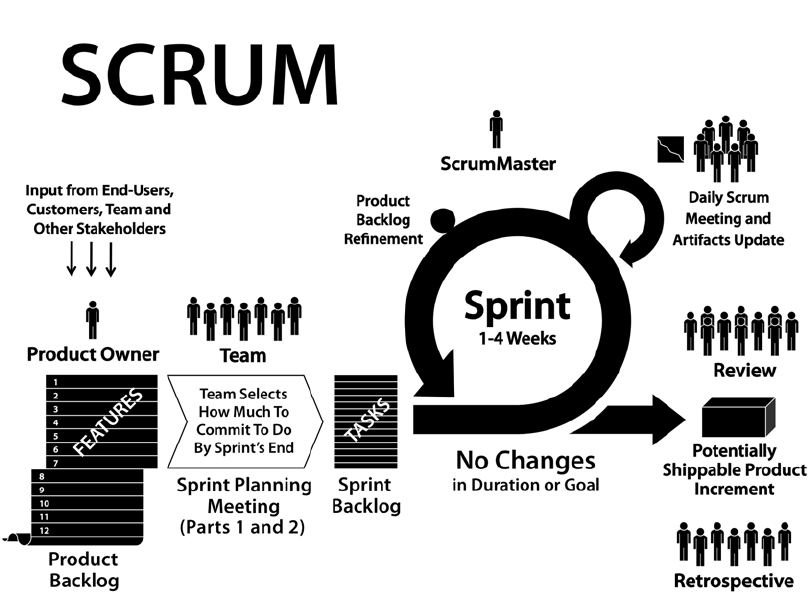
\includegraphics[width=15cm]{figuras/Scrum.png}}
\caption{Metodoloxía Scrum}
\medskip
\small
\centerline{Fonte: \cite{ScrumPrimer}}
\label{ScrumFigure}
\end{figure}

\subsection{Planificación temporal}

Como xa foi explicado, a metodoloxía a empregar neste proxecto trátase da metodoloxía áxil Scrum, na que será posíbel escoller unha tarefa ou serie de tarefas cada vez que se realice un novo \textit{sprint}, e que pretende dar resposta a un nivel grande de incerteza. Ademais, é moi probábel que novas tarefas sexan engadidas á lista de tarefas a medida que o proxecto avanza e vaise dando resposta a certos termos que non resultan claros dende o comezo. Porén, achouse innecesaria a realización dunha planificación temporal ao comezo do proxecto, unha perspectiva enfocada ás metodoloxías pesadas ou clásicas, onde todos os requisitos xa están definidos dende o comezo do proxecto. Deste xeito, enténdese que, aínda seguindo unha estrutura xeral, que será exposta na \gls{EDT} presentada na sección \ref{EDTT}, será posíbel e probábel que xurdan novos requisitos a medida que son cumpridos os requisitos de maior importancia, o que fai realmente complicada a realización dunha planificación temperá con exactitude.\\

Asumindo polo tanto o nivel de incerteza ao que se afronta o proxecto, sobre todo no seu comezo, considérase que non é factíbel a realización dunha planificación temporal extensa, ao non ter coñecemento de todos os requisitos que poderán xurdir a medida que o mesmo avance.\\

Deste xeito, tendo en conta as argumentacións anteriores, conclúese que non paga a pena a realización dun diagrama de Gantt para a realización dunha planificación temporal exhaustiva.

\subsection{Estrutura de detalle do traballo}
\label{EDTT}

Aínda existindo un grande nivel de incerteza e non sendo factíbel a realización dunha planificación temporal exhaustiva, si que resulta posíbel incluso dende o comezo do proxecto, a realización dunha división do traballo a realizar en diferentes módulos. Así, realizarase unha \gls{EDT}, que atendendo ao PMBOK \cite{PMBOK}, outorga unha visión global dende o máis xeral ao máis específico do alcance do proxecto e amosa dun xeito xerárquico o traballo que é preciso realizar para a súa realización. Dita \gls{EDT} está representada na figura \ref{EDTTFigura}.

\begin{figure}
\centerline{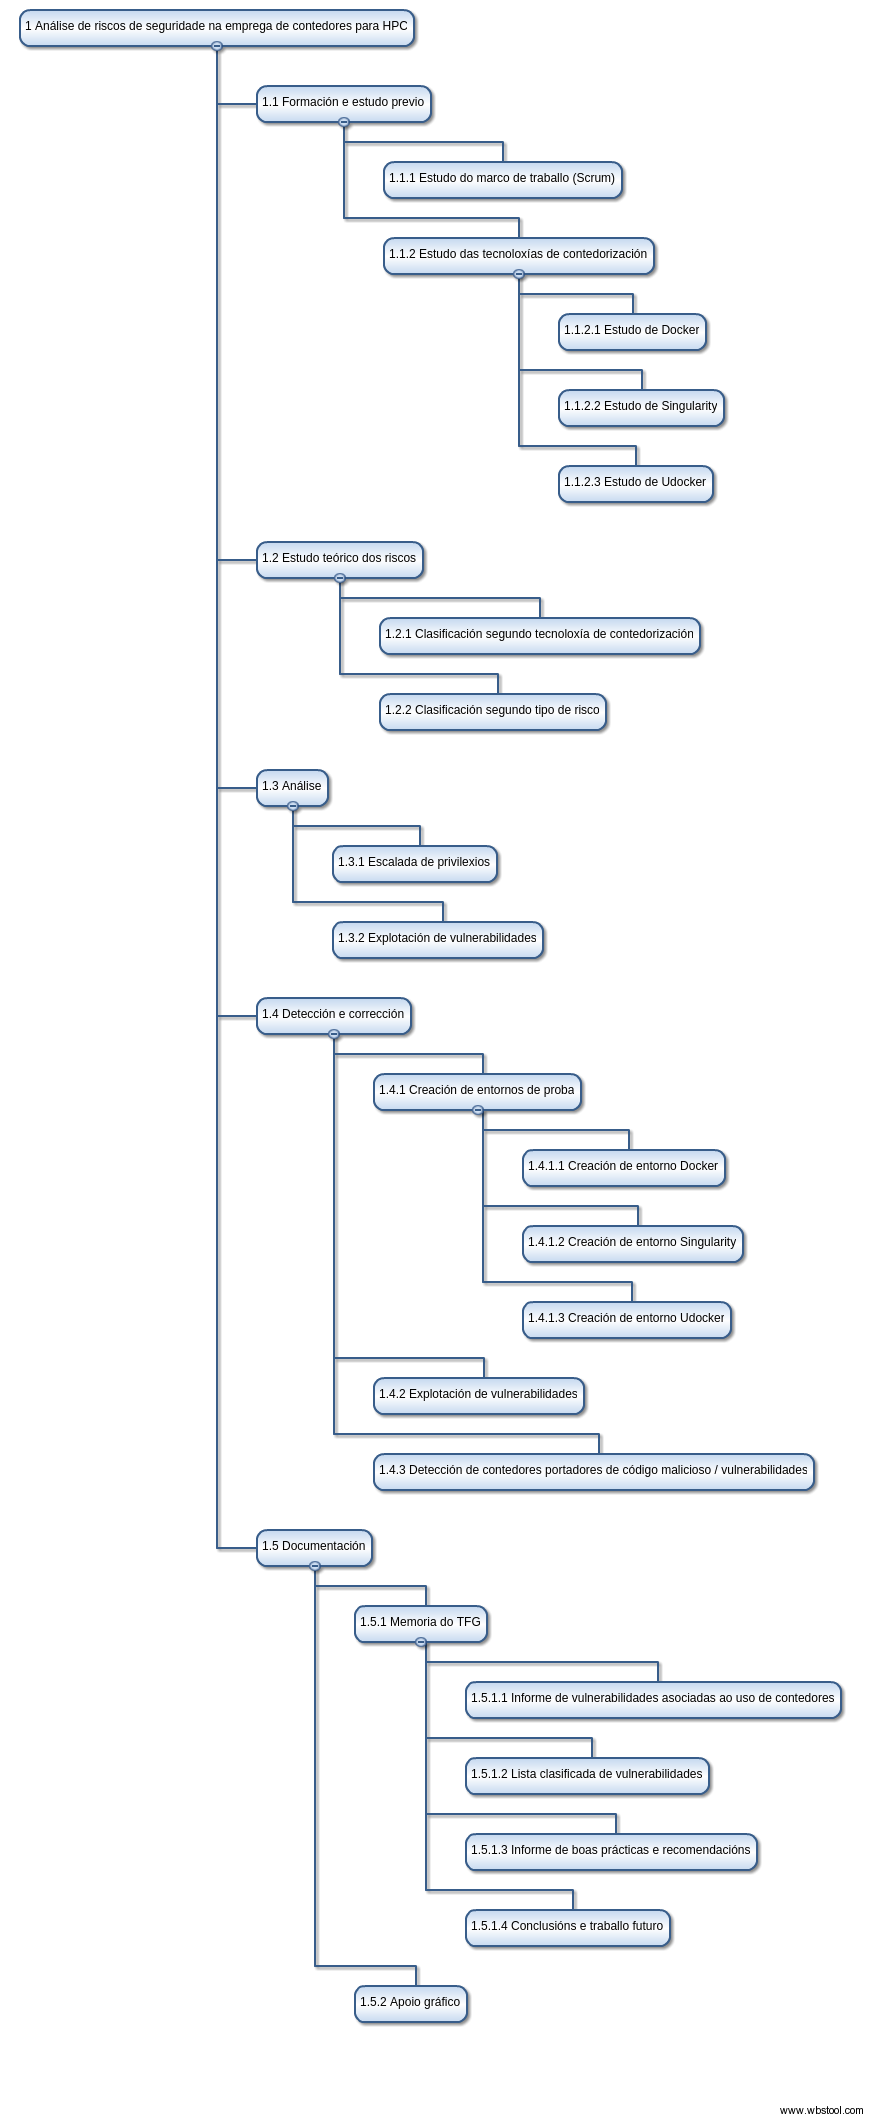
\includegraphics[width=9cm]{figuras/EDTT.png}}
\caption{\gls{EDT} do proxecto}
\label{EDTTFigura}
\end{figure}

\subsection{División temporal xeral das principais fases do proxecto}
\label{divisionTemporalXeral}

Xa foi explicado que resulta complicado realizar unha estruturación temporal detallada do proxecto. Non obstante, contando co detalle de traballo do proxecto, representada na \gls{EDT} da sección \ref{EDTT}, e asumindo as grandes limitacións de tempo ás que se afronta este proxecto, xa que presenta un tempo de desenvolvemento máximo de 412.5 horas, si que resulta posíbel realizar unha división temporal xeneralizada a alto nivel sobre as fases principais do proxecto. O traballo semanal previsto é dunhas 24 horas semanais. O estudo resultante é o seguinte:

\subsubsection{Formación e estudo previo}

\begin{itemize}
    \item \textbf{Duración:} 2 semanas.
    \item \textbf{Descrición:} a pesar de que o autor xa posúe experiencia tratando con tecnoloxías de contedorización, será preciso que revise os seus coñecementos. Tamén cómpre que o autor entenda e interiorice os trazos principais da metodoloxía de traballo, para poder póla en práctica ao longo do proxecto.
\end{itemize}

\subsubsection{Estudo teórico dos riscos}

\begin{itemize}
    \item \textbf{Duración:} 2 semanas.
    \item \textbf{Descrición:} aínda que o autor deste proxecto xa conta con experiencia previa no traballo con tecnoloxías de contedorización, é preciso que adique unha cantidade de tempo razoábel á lectura de artigos referentes á seguridade dos mesmos ou doutras tecnoloxías de virtualización, co fin de identificar os riscos existentes neste eido. A medida que o estudo avance, realizarase unha clasificación, tanto segundo a tecnoloxía como segundo o tipo de risco (rede, explotación de vulnerabilidades, etc.)
    
    É moi probábel que a medida que se investiguen diferentes aspectos relacionados coa seguridade desta tecnoloxía sexa preciso procurar información novamente, sobre temas máis específicos ou facer varias repeticións para asegurar o seu correcto entendemento. Isto quere dicir que é posíbel que esta fase, nun principio introdutoria, esténdase ao longo da totalidade do proxecto.
\end{itemize}

\subsubsection{Análise}

\begin{itemize}
    \item \textbf{Duración:} 4 semanas
    \item \textbf{Descrición:} realizada unha detección dos riscos asociados ás tecnoloxías de contedorización, cómpre realizar unha análise intensiva dos mesmos. Nesta sección realizarase un estudo principalmente teórico, inspirado noutros estudos e artigos científicos xa desenvolvidos pola comunidade. Tamén abarcará o achegamento dun estudo máis empírico mediante probas sobre os entornos de pre-produción e produción para efectuar noutra fase do proxecto.
\end{itemize}

\subsubsection{Detección e corrección}

\begin{itemize}
    \item \textbf{Duración:} 6 semanas.
    \item \textbf{Descrición:} nesta fase crearanse os entornos de proba para poder realizar un estudo empírico das diferentes vulnerabilidades atopadas en etapas anteriores. Inclúe a instalación e despregamento de ferramentas externas para dito estudo, como por exemplo a configuración de ferramentas para a detección de vulnerabilidades en imaxes.
    
    Do mesmo xeito, serán efectuadas diversas probas para evidenciar os riscos aos que se expón un sistema baseado en contedores. Esta fase estará amplamente ligada coa fase de formación e análise, confluíndo probabelmente no tempo, a medida que o factor de incerteza se vai reducindo.
\end{itemize}

\subsubsection{Documentación}

\begin{itemize}
    \item \textbf{Duración:} 3 semanas
    \item \textbf{Descrición:} esta fase supón a redacción da actual memoria, así como a elaboración de todos as figuras e gráficos precisos para a realización de explicacións visuais. Supón á súa vez o contido do traballo, ao non ser un traballo de desenvolvemento software, posto que non existe a penas código (limitado aos \textit{scripts} de configuración ou probas).
    
    É por tanto unha das partes máis cruciais do proxecto, pois é onde deben quedar reflectidos todos os avances feitos. Seguramente tamén teña lugar de xeito paralelo con outras fases, para non esquecer ou perder a información obtida.
\end{itemize}

\section{Presupostos}

Esta sección terá como obxectivo a elaboración dos presupostos do proxecto. Para tal fin, farase unha división entre custos materiais e custos asociados aos recursos humanos. Ademais, tamén debemos diferenciar:

\begin{itemize}
    \item \textbf{Custos directos:} vinculados exclusivamente co desenvolvemento deste proxecto.
    \item \textbf{Custos indirectos:} repartidos entre diferentes proxectos desenvolvidos no mesmo lugar de traballo. Xeralmente son calculados como unha porcentaxe dos custos directos. Un exemplo é o consumo de luz ou auga.
\end{itemize}

\subsection{Custos directos}

\subsubsection{Custos materiais}
\label{custosMateriaisDirectos}

O listado de custos materiais precisos para o desenvolvemento deste proxecto son:

\begin{itemize}
    \item \textbf{Equipo de traballo:} composto por un ordenador de sobremesa, pantalla, teclado e rato. Estímase un valor total duns 1000\euro, e unha vida media duns 6 anos para dito equipo. Tendo en conta a duración deste proxecto, o custo do equipo é de 55.56\euro, tal e como amosan os cálculos da táboa \ref{custoEquipoTraballo}.
    
    \begin{table}[H]
    \centering
    \caption{Custo calculado do equipo de traballo}
    \label{custoEquipoTraballo}
    \begin{tabular}{|c|c|c|c|}
    \hline
    Meses de vida & Meses de uso no proxecto & Custo total & Custo no proxecto \\ \hline
    72 & 4 & 1000\euro & 55.56\euro \\ \hline
    \end{tabular}
    \end{table}
    
    \item \textbf{Material funxíbel:} material físico para a realización do proxecto como bolígrafos, carpetas, cadernos, fotocopias, etc. Estímase nuns 20\euro.
    \item \textbf{Software:} todo o software a empregar ao longo do proxecto será libre ou, ao menos, de balde, polo que non suporá ningún custo no proxecto. Polo tanto, isto limitará a tecnoloxía de Docker á edición \textit{Community Edition} (CE), a cal é gratuíta, quedando descartada a edición \textit{Enterprise Edition} (EE), de pago.
    \item \textbf{Custos computacionais do \gls{FT2}:} no desenvolvemento do proxecto farase uso dos medios computacionais do \gls{CESGA}. Aínda que estes son recursos compartidos, existen medidas que permiten a reserva de recursos limitados, cos que a súa contabilización será moito máis sinxela. O custo aproximado de utilización dos recursos é duns 3 céntimos de euro por procesador por minuto. Tendo en conta as probas que será preciso realizar, estímase a emprega duns 12 procesadores (distribuídos en varias máquinas virtuais), durante unhas 70 horas, polo que os gastos totais asociados a computación ascenderían a 1512\euro.
\end{itemize}

Os custos directos asociados aos materiais do proxecto poden ser consultados na táboa \ref{custosDirectosMateriais}.

\begin{table}[]
\centering
\caption{Custos directos asociados aos materiais}
\label{custosDirectosMateriais}
\begin{tabular}{|c|c|}
\hline
\textbf{Nome} & \textbf{Custo} \\ \hline
Equipo de traballo & 55.56\euro \\ \hline
Material funxíbel & 20\euro \\ \hline
Software & 0\euro \\ \hline
Custos computacionais & 1512\euro \\ \hline \hline
\textbf{TOTAL} & \textbf{1587.56\euro} \\ \hline
\end{tabular}
\end{table}

\subsubsection{Custos de persoal}
\label{custosPersoaisDirectos}

Para realizar o cálculo dos custos asociados aos \gls{RRHH} involucrados no desenvolvemento deste proxecto, cómpre diferenciar os diferentes roles que toman parte no mesmo. Podemos distinguir:

\begin{itemize}
    \item \textbf{Director do proxecto:} rol asumido por ambos os dous titores do proxecto, tendo como labor a supervisión do mesmo e a titorización. Sumaranse as horas de ambos para o cálculo total.
    \item \textbf{Xefe do proxecto:} o seu labor e a redacción da memoria, a corrección da mesma, planificación temporal, análise de riscos, presupostos, etc.
    \item \textbf{Asistente á investigación:} o seu labor consiste na investigación de vulnerabilidades en entornos de contedores para \gls{HPC}, así como en reflectir todos os avances atopados e probas na memoria.
\end{itemize}

Para o cálculo dos salarios empregarase a ferramenta en liña Experteer\footnote{\url{https://www.experteer.es/}} para obter o salario bruto anual e asumirase un custo dun 32\% para o cálculo da Seguridade Social.  A partir desas medidas calcularanse os custos por este proxecto, asumindo un total 14 pagas ao ano e unha xornada laboral 8 horas diarias e 20 días laborábeis ao mes. Os cálculos poden ser observados na táboa \ref{calculoSalarios}.

\begin{table}[H]
\centering
\caption{Cálculo dos salarios dos diferentes roles do proxecto}
\label{calculoSalarios}
\resizebox{\textwidth}{!}{%
\begin{tabular}{|l|c|c|c|c|c|}
\hline
\textbf{Rol} & \textbf{Bruto anual} & \textbf{Seguridade Social} & \textbf{Total anual} & \textbf{Total mensual} & \textbf{Custo/hora} \\ \hline
Director do proxecto & 38000\euro & 12160\euro & 50160\euro & 3583\euro & 22.39\euro \\ \hline
Xefe do proxecto & 32000\euro & 10240\euro & 42240\euro & 3017\euro & 18.86\euro \\ \hline
Asistente á investigación & 17000\euro & 5440\euro & 22440\euro & 1603\euro & 10.01\euro \\ \hline
\end{tabular}
}
\end{table}

Obtidos os diferentes custos por hora, é posíbel deducir os gastos directos asociados aos \gls{RRHH} deste proxecto, que poden ser consultados na táboa \ref{custosDirectosRRHH}.

\begin{table}[H]
\centering
\caption{Custos directos asociados aos \gls{RRHH}}
\label{custosDirectosRRHH}
\begin{tabular}{|l|c|c|c|}
\hline
\textbf{Rol} & \textbf{Custo/hora }& \textbf{Número de horas} & \textbf{Custo total} \\ \hline
Director do proxecto & 22.39\euro & 20 & 447.80\euro \\ \hline
Xefe do proxecto & 18.86\euro & 90 & 1697.40\euro \\ \hline
Asistente á investigación & 10.01\euro & 310 & 3103.10\euro \\ \hline \hline
\textbf{TOTAL} & \multicolumn{2}{l|}{} & \textbf{5248.30\euro} \\ \hline
\end{tabular}
\end{table}

\subsubsection{Custos directos totais}

Obtidos os custos directos materiais (\ref{custosMateriaisDirectos}) e de persoal (\ref{custosPersoaisDirectos}), podemos obter o total dos custos directos, que ascende a un \textbf{total de 6835.86\euro}.

\begin{table}[H]
\centering
\caption{Custos directos totais}
\label{custosDirectosTotais}
\begin{tabular}{|l|c|}
\hline
\textbf{Tipo} & \textbf{Custo asociado} \\ \hline
Material & 1587.56\euro \\ \hline
Persoal & 5248.30\euro \\ \hline \hline
\textbf{TOTAL} & \textbf{6835.86\euro} \\ \hline
\end{tabular}
\end{table}

\subsection{Custos indirectos}

Tendo en conta o marco no que se desenvolve este proxecto, realizado no \gls{CESGA} e no Departamento de Electrónica e Computación da Universidade de Santiago de Compostela, decidiuse seguir as políticas de custos en I+D da Universidade \cite{xestionEconomicaUSC}, a cal indica que se deben calcular tomando como referencia un 20\% dos custos directos totais. Deste xeito, os custos indirectos ascenden a un \textbf{total de 1307.12\euro}.

\subsection{Custos totais}

Os custos totais calcúlanse como a suma dos custos directos e indirectos. Os custos totais deste proxecto ascenden a un \textbf{total de 8143.03\euro}.

\begin{table}[H]
\centering
\caption{Custos totais}
\label{custosTotais}
\begin{tabular}{|l|c|}
\hline
\textbf{Tipo} & \textbf{Custo asociado} \\ \hline
Directo & 6835.86\euro \\ \hline
Indirecto & 1307.12\euro \\ \hline \hline
\textbf{TOTAL} & \textbf{8143.03\euro} \\ \hline
\end{tabular}
\end{table}

\section{Alcance do proxecto}

\subsection{Descrición do alcance}

O presente proxecto ten como finalidade o estudo de vulnerabilidades na emprega de contedores para \gls{HPC}. Tal cometido entenderase rematado coa obtención dunha lista clasificada de vulnerabilidades, un estudo das mesmas, unha documentación de boas prácticas e recomendacións así como unha serie de conclusións e traballo futuro para a posíbel continuidade do proxecto.

\subsection{Entregábeis do proxecto}

Os entregábeis deste proxecto consisten nesta propia memoria, con todos os estudos xa realizados e as conclusións obtidas, así como todos as figuras realizadas para a súa explicación visual e os \textit{scripts} precisos para a reproducibilidade das probas.

\subsection{Exclusións do proxecto}

Quedarán descartadas aquelas tarefas que pola súa complexidade incrementen notabelmente o tempo planificado para a execución da división temporal xeral das principais fases do proxecto, establecidas na sección \ref{divisionTemporalXeral}. Non debemos esquecer que este se trata dun proxecto asociado a un Traballo de Fin de Grao, polo que a súa limitación temporal é moi forte e debe ser respectada.

\subsection{Supostos do proxecto}

Asúmese que dende o comezo do proxecto o autor deste proxecto contará con acceso a todos os medios necesarios para realizar as probas que considere precisas (acceso aos entornos de pre-produción e produción).

\subsection{Restricións do proxecto}

\begin{itemize}
    \item Duración máxima do proxecto: 4 meses.
    \item Data máxima de entrega da memoria: 2 de xullo de 2018.
\end{itemize}

\cleardoublepage
\chapter{Especificación de requisitos}
\minitoc
\clearpage

\section{Limitacións}

Este capítulo está adicado á recollida e especificación de requisitos que debe cumprir o proxecto. Non obstante, ao non ser un proxecto de desenvolvemento software, esta análise deberá ser adaptada como se indica a continuación:

\begin{itemize}
    \item \textbf{No referente aos casos de uso:} a extracción de casos de uso é unha técnica amplamente empregada no desenvolvemento de software para a obtención de información no referente ao que o sistema debe facer a alto nivel. No entanto, ao non existir un desenvolvemento software na realización deste proxecto, non será posíbel obter ou definir casos de uso.
    
    \item \textbf{No referente aos actores:} podemos definir aos actores como representacións dos usuario que van empregar o sistema. Novamente, ao non existir un sistema software a desenvolver, non ten sentido a definición de actores neste proxecto.
    
    \item \textbf{No referente aos requisitos funcionais:} os requisitos funcionais fan referencia ás funcionalidades que definen o software tal e como o usuario final ou o cliente o entenden. Polos mesmos motivos, non será factíbel a definición de requisitos funcionais.
    
    \item \textbf{No referente á matriz de trazabilidade:} a matriz de trazabilidade relaciona os casos de uso cos requisitos funcionais. Ao non existiren nin uns nin outros, non é posíbel a creación da mesma.

    \item \textbf{No referente aos requisitos non funcionais:} os requisitos non funcionais son aqueles que, se ben indican requirimentos a acadar na realización do proxecto, non poden ser considerados coma funcionalidades. Polo tanto, estes son os tipos de requisitos que terá este proxecto.
\end{itemize}

\section{Requisitos non funcionais}

Para o estudo dos requisitos non funcionais, primeiramente farase un listado dos mesmos, seguindo as indicacións do \gls{CESGA} para a realización do proxecto. Posteriormente realizarase unha explicación dos mesmos polo miúdo, ademais de indicar a importancia que se lles confire no proxecto.

\subsection{Listado de requisitos non funcionais}

\begin{enumerate}[{RNF}1: ]
    \item Realización do estudo de seguridade con 3 tecnoloxías de contedorización: Docker, Singularity e Udocker.
    \item Detección de riscos de seguridade na emprega de contedores nun entorno \gls{HPC}.
    \item Clasificación de riscos de seguridade segundo o tipo de tecnoloxía de contedorización na emprega de contedores nun entorno \gls{HPC}.
    \item Clasificación de riscos de seguridade segundo a súa natureza na emprega de contedores nun entorno \gls{HPC}.
    \item Estudo teórico dos riscos de seguridade.
    \item Estudo práctico dos riscos de seguridade.
    \item Definición dun método para a detección de vulnerabilidades en imaxes.
    \item Definición dun mecanismo de validación de imaxes.
    \item Estudo da limitación dos recursos na emprega de contedores.
    \item Estudo do reforzamento da seguridade mediante a emprega de medidas externas.
    \item Redacción de boas prácticas e recomendacións para a correcta emprega de contedores nun entorno \gls{HPC}.
    \item Emprega de software libre ou de balde.
\end{enumerate}

\subsection{Explicación dos requisitos non funcionais}

\begin{table}[H]
\centering
\caption{Requisito non funcional RNF1}
\label{RNF1}
\begin{tabularx}{\textwidth}{|l|X|}
\hline
\textbf{ID} & RNF1 \\ \hline
\textbf{Nome} & Realización do estudo de seguridade con 3 tecnoloxías de contedorización: Docker, Singularity e Udocker. \\ \hline
\textbf{Descrición} & Será preciso estudar diferentes tecnoloxías de contedorización, co fin de detectar as vantaxes que presentan as unhas sobre as outras no referente á seguridade. \\ \hline
\textbf{Importancia} & Vital \\ \hline
\end{tabularx}
\end{table}

\begin{table}[H]
\centering
\caption{Requisito non funcional RNF2}
\label{RNF2}
\begin{tabularx}{\textwidth}{|l|X|}
\hline
\textbf{ID} & RNF2 \\ \hline
\textbf{Nome} & Detección de riscos de seguridade na emprega de contedores nun entorno \gls{HPC}. \\ \hline
\textbf{Descrición} & Descubrir cales poderían ser os posíbeis vectores de ataque e debilidades na seguridade no uso de contedores. \\ \hline
\textbf{Importancia} & Vital \\ \hline
\end{tabularx}
\end{table}

\begin{table}[H]
\centering
\caption{Requisito non funcional RNF3}
\label{RNF3}
\begin{tabularx}{\textwidth}{|l|X|}
\hline
\textbf{ID} & RNF3 \\ \hline
\textbf{Nome} & Clasificación de riscos de seguridade segundo o tipo de tecnoloxía de contedorización na emprega de contedores nun entorno \gls{HPC}. \\ \hline
\textbf{Descrición} & Xa detectados riscos, clasificalos segundo o tipo de tecnoloxía de contedorización, axudando a completar o RNF1. \\ \hline
\textbf{Importancia} & Vital \\ \hline
\end{tabularx}
\end{table}

\begin{table}[H]
\centering
\caption{Requisito non funcional RNF4}
\label{RNF4}
\begin{tabularx}{\textwidth}{|l|X|}
\hline
\textbf{ID} & RNF4 \\ \hline
\textbf{Nome} & Clasificación de riscos de seguridade segundo a súa natureza na emprega de contedores nun entorno \gls{HPC}. \\ \hline
\textbf{Descrición} & Xa detectados riscos, clasificalos segundo a súa natureza, para permitir un posterior estudo: rede, escalada de privilexios, denegación de servizo, etc. \\ \hline
\textbf{Importancia} & Vital \\ \hline
\end{tabularx}
\end{table}

\begin{table}[H]
\centering
\caption{Requisito non funcional RNF5}
\label{RNF5}
\begin{tabularx}{\textwidth}{|l|X|}
\hline
\textbf{ID} & RNF5 \\ \hline
\textbf{Nome} & Estudo teórico dos riscos de seguridade. \\ \hline
\textbf{Descrición} & Xa detectados e clasificados os riscos, realizar un estudo teórico dos mesmos, para comprender o perigo asociado á súa existencia. Nalgúns casos, este estudo teórico abondará. \\ \hline
\textbf{Importancia} & Vital \\ \hline
\end{tabularx}
\end{table}

\begin{table}[H]
\centering
\caption{Requisito non funcional RNF6}
\label{RNF6}
\begin{tabularx}{\textwidth}{|l|X|}
\hline
\textbf{ID} & RNF6 \\ \hline
\textbf{Nome} & Estudo práctico dos riscos de seguridade. \\ \hline
\textbf{Descrición} & Realizado o estudo teórico, farase unha posta en práctica na que se explotarán certas vulnerabilidades achadas, evidenciando o seu perigo para o sistema. \\ \hline
\textbf{Importancia} & Desexábel \\ \hline
\end{tabularx}
\end{table}

\begin{table}[H]
\centering
\caption{Requisito non funcional RNF7}
\label{RNF7}
\begin{tabularx}{\textwidth}{|l|X|}
\hline
\textbf{ID} & RNF7 \\ \hline
\textbf{Nome} & Definición dun método para a detección de vulnerabilidades en imaxes. \\ \hline
\textbf{Descrición} & Procurarase un mecanismo que permita a procura de vulnerabilidades en imaxes, probabelmente baseado na emprega de ferramentas xa existentes. Será preciso realizar unha explicación do seu funcionamento. \\ \hline
\textbf{Importancia} & Vital \\ \hline
\end{tabularx}
\end{table}

\begin{table}[H]
\centering
\caption{Requisito non funcional RNF8}
\label{RNF8}
\begin{tabularx}{\textwidth}{|l|X|}
\hline
\textbf{ID} & RNF8 \\ \hline
\textbf{Nome} & Definición dun mecanismo de validación de imaxes. \\ \hline
\textbf{Descrición} & Procura e explicación dun método que permita garantir a validación das imaxes. Isto é, garantir aspectos como autenticación integridade e non repudio. \\ \hline
\textbf{Importancia} & Vital \\ \hline
\end{tabularx}
\end{table}

\begin{table}[H]
\centering
\caption{Requisito non funcional RNF9}
\label{RNF9}
\begin{tabularx}{\textwidth}{|l|X|}
\hline
\textbf{ID} & RNF9 \\ \hline
\textbf{Nome} & Estudo da limitación dos recursos na emprega de contedores. \\ \hline
\textbf{Descrición} & Procura de mecanismos que permitan limitar os recursos a empregar por un contedor. Explicación do seu funcionamento. \\ \hline
\textbf{Importancia} & Vital \\ \hline
\end{tabularx}
\end{table}

\begin{table}[H]
\centering
\caption{Requisito non funcional RNF10}
\label{RNF10}
\begin{tabularx}{\textwidth}{|l|X|}
\hline
\textbf{ID} & RNF10 \\ \hline
\textbf{Nome} & Estudo do reforzamento da seguridade mediante a emprega de medidas externas. \\ \hline
\textbf{Descrición} & Investigación de medidas externas (alleas ás propias tecnoloxías de contedorización) que permitan engadir unha capa de seguridade no sistema, de xeito que este resulte máis seguro no seu conxunto para a emprega de contedores. \\ \hline
\textbf{Importancia} & Desexábel \\ \hline
\end{tabularx}
\end{table}

\begin{table}[H]
\centering
\caption{Requisito non funcional RNF11}
\label{RNF11}
\begin{tabularx}{\textwidth}{|l|X|}
\hline
\textbf{ID} & RNF11 \\ \hline
\textbf{Nome} & Redacción de boas prácticas e recomendacións para a correcta emprega de contedores nun entorno \gls{HPC}. \\ \hline
\textbf{Descrición} & Finalizado o estudo sobre os riscos de seguridade na emprega de contedores en \gls{HPC}, serán explicadas unha serie de prácticas que permitan mellorar a seguridade destes entornos. \\ \hline
\textbf{Importancia} & Desexábel \\ \hline
\end{tabularx}
\end{table}

\begin{table}[H]
\centering
\caption{Requisito non funcional RNF12}
\label{RNF12}
\begin{tabularx}{\textwidth}{|l|X|}
\hline
\textbf{ID} & RNF12 \\ \hline
\textbf{Nome} & Emprega de software libre ou de balde. \\ \hline
\textbf{Descrición} & O software a empregar ao longo do desenvolvemento deste proxecto debe ser libre ou de balde. Por esta razón, quedará fóra do estudo a versión \textit{Enterprise Edition} de Docker, a cal é unha solución comercial non gratuíta. \\ \hline
\textbf{Importancia} & Vital \\ \hline
\end{tabularx}
\end{table}

\cleardoublepage
%\chapter{Deseño}

Deseño: cómo se realiza o Sistema, a división deste en diferentes compoñentes e a comunicación entre eles. Así mesmo, determinarase o equipamento hardware e software necesario, xustificando a súa elección no caso de que non fora un requisito previo. Debe achegarse a un nivel suficiente de detalle que permita comprender a totalidade da estrutura do produto desenvolvido, utilizando no  posible representacións gráficas.

%\cleardoublepage
\chapter{Infraestrutura}
\minitoc
\clearpage

\section{Contextualización}

O desenvolvemento deste proxecto está contextualizado no \gls{CESGA}, o centro de cálculo, comunicacións de altas prestacións e servizos avanzados da Comunidade Científica Galega, do Sistema Académico Universitario e do Consello Superior de Investigacións Científicas (CSIC). Cómpre coñecer as singularidades que un centro \gls{HPC} posúe no tratamento con contedores, polo que a súa infraestrutura e a relación con esta tecnoloxía de virtualización serán explicadas polo miúdo neste capítulo.

\section{Finis Terrae II}
\label{recursosFT2}

Finis Terrae II é un sistema de computación xestionado polo \gls{CESGA} e integrado na Rede Española de Supercomputación, considerada unha Infraestrutura Científica e Técnica Singular (ICTS). Trátase dun \textit{cluster} Linux heteroxéneo, baseado en procesadores Intel Haswell e interconectado mediante rede InfiniBand cun rendemento pico de 328 TFlops e sostido en Linpack de 213 Tflops. Posúe unha rede de Interconexión de alto rendemento Mellanox InfiniBand FDR@56Gbps con topoloxía \textit{Fat-tree} e un sistema de ficheiros paralelo Lustre con 768TB de capacidade (750TB netos) e 20GB/s de lectura/escritura cun consumo total de 118Kw e rendemento pico de 328 TFlops (240 Tflops Linpack) \cite{FT2CESGA}. Unha representación de dita arquitectura pode ser apreciada nas figuras \ref{FT2_1}, \ref{FT2_2}, \ref{FT2_3} e \ref{InfiniBandFigura}.

\begin{figure}
\centerline{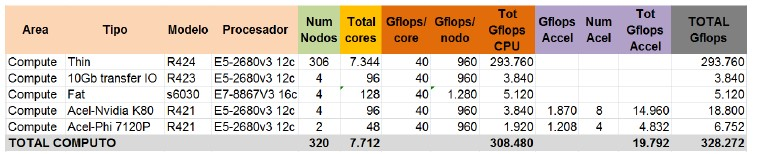
\includegraphics[width=15cm]{figuras/FT2_1.jpg}}
\caption{Arquitectura do \gls{FT2}. Parte 1.}
\medskip
\small
\centerline{Fonte: \url{https://cesga.es/gl/infraestructuras/computacion/FinisTerrae2}}
\label{FT2_1}
\end{figure}

\begin{figure}
\centerline{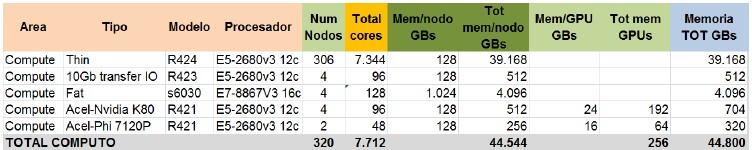
\includegraphics[width=15cm]{figuras/FT2_2.jpg}}
\caption{Arquitectura do \gls{FT2}. Parte 2.}
\medskip
\small
\centerline{Fonte: \url{https://cesga.es/gl/infraestructuras/computacion/FinisTerrae2}}
\label{FT2_2}
\end{figure}

\begin{figure}
\centerline{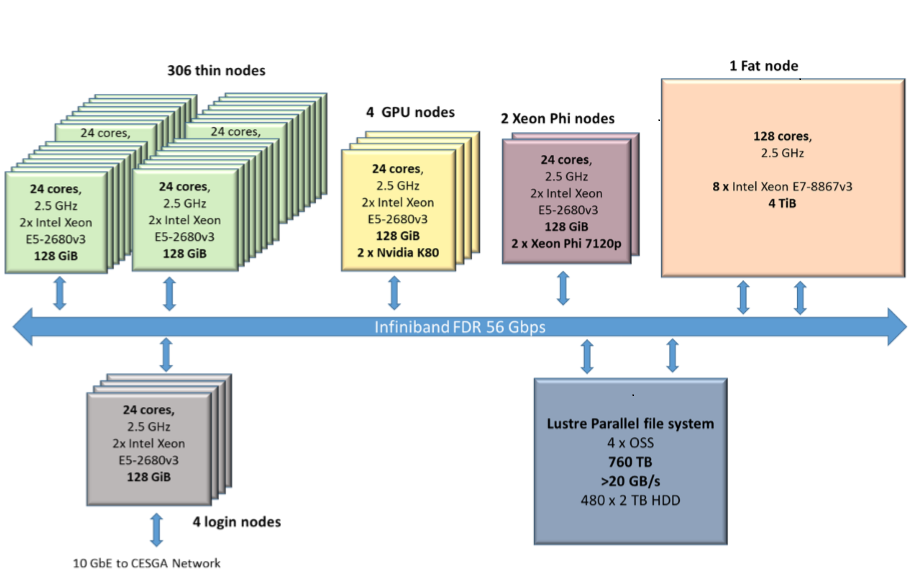
\includegraphics[width=15cm]{figuras/infraFTII.png}}
\caption{Arquitectura do \gls{FT2}. Parte 3.}
\medskip
\small
\centerline{Fonte: \cite{MSO4SC}}
\label{FT2_3}
\end{figure}

\begin{figure}
\centerline{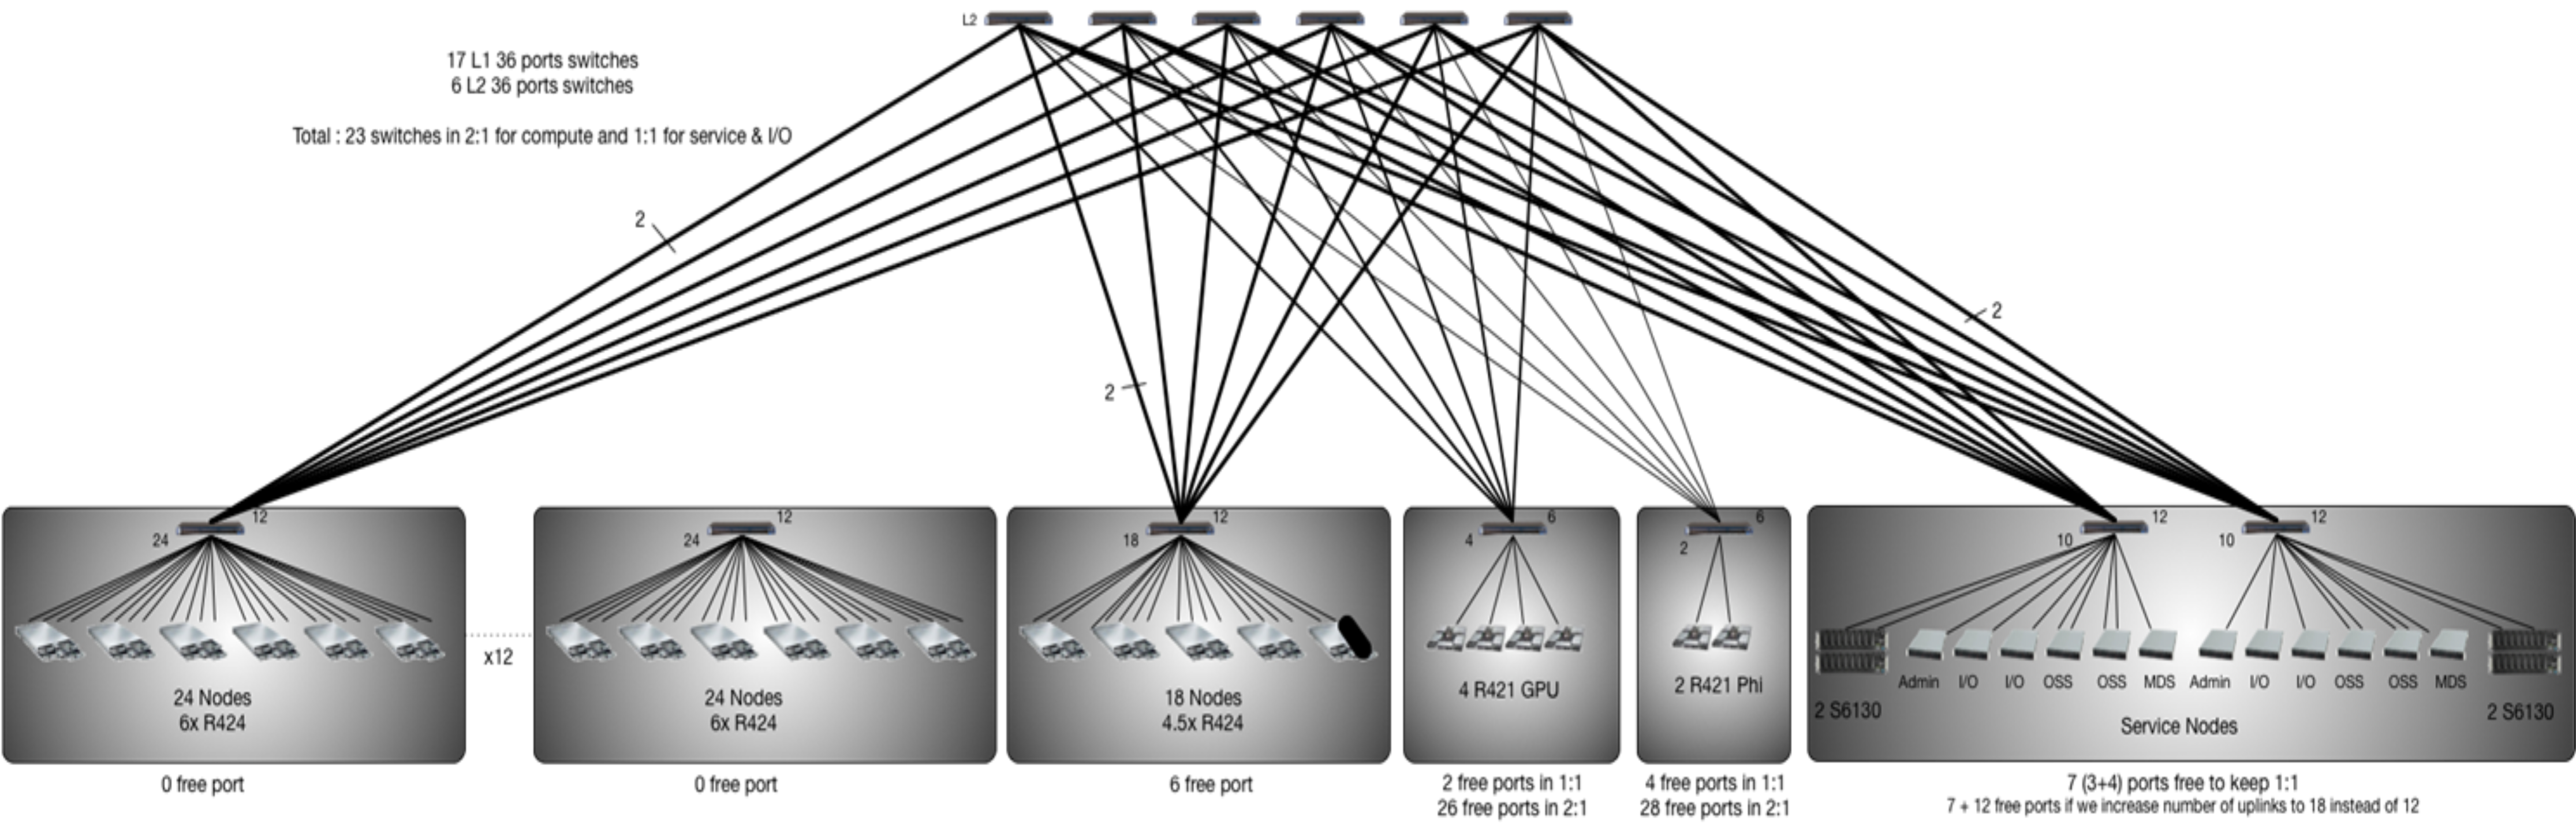
\includegraphics[width=15cm]{figuras/InfiniBand.png}}
\caption{Diagrama da rede InfiniBand do \gls{FT2}}
\medskip
\small
\centerline{Fonte: \url{https://cesga.es/gl/infraestructuras/computacion/FinisTerrae2}}
\label{InfiniBandFigura}
\end{figure}

\section{Contedores e \gls{HPC}}

A emprega de contedores permite a execución de múltiples entornos baixo unha máquina anfitrioa común, o cal supón un mellor aproveitamento do sistema e a posibilidade de establecer separacións máis claras sobre os diferentes procesos. Estas vantaxes tamén son aportadas por outras tecnoloxías de virtualización, como poden ser as máquinas virtuais; no entanto, o uso de contedores supón outra serie de melloras como pode ser a compartición do \textit{kernel} coa máquina anfitrioa, empregando soamente capas lixeiras para o sistema operativo \cite{OS-level-security}. Como resultado, a virtualización a nivel de sistema operativo supón unha perda de rendemento moito menor en comparación con outras tecnoloxías de virtualización, que poden chegar a ser consideradas desprezábeis. Tamén debemos ter en conta que cando traballamos con máquinas virtuais estamos a crear sistemas cuns límites moi definidos (en termos de CPU, memoria e demais recursos), que deben ser restruturados se os queremos ampliar e que moi probabelmente non sexan empregados na súa totalidade, ou ao menos na meirande parte do tempo. Non obstante, a emprega de contedores permite uns límites máis laxos que se adaptan aos recursos dispoñíbeis, contando coa vantaxe de poder establecer uns límites máximos en moitos dos casos, dependendo da tecnoloxía de virtualización.\\

Este achegamento do rendemento a niveis practicamente nativos fai dos contedores unha alternativa moi a ter en conta en entornos de computación de altas prestacións, xunto cos seguintes motivos:

\begin{itemize}
    \item \textbf{Desenvolvemento áxil:} o desenvolvemento tradicional de software en entornos \gls{HPC} presenta algunhas características que o fan moi inflexíbel. O desenvolvemento e integración tradicionais de software baséanse na realización de todos os pasos precisos, como a descarga, configuración, construción, realización de probas e instalación, para ter o software correndo na infraestrutura de produción. Cando traballamos con software científico debemos ter en conta que acostuma ser un software extremadamente complexo dende o punto de vista arquitectónico. Adoita incluír numerosos conceptos e características matemáticas implantados ao longo de varios compoñentes software para prover capas de abstracción a alto nivel. Ditas capas poden estar implantadas directamente no proxecto de software ou integradas a través de librarías de terceiros, polo que o entorno enteiro de software científico supón finalmente unha composición complexa de matrices de dependencias entre diferentes programas e librarías. Todo este proceso pode ser simplificado se empaquetamos todas as librarías e dependencias precisas dentro dun contedor, sobre todo se temos en conta que o proceso de despregamento dun contedor resulta relativamente áxil grazas ao seu pequeno tamaño.
    
    Tamén debe ser tido en conta que certos programas evolucionan moi rápido, empregando últimas tecnoloxías e dependencias difíciles de satisfacer, ao levar esta elevada frecuencia de actualización. Tal tarefa exerce moita presión sobre o equipo de soporte de software de infraestruturas multiusuario como pode ser o \gls{CESGA}.
    
    \item \textbf{Illamento:} o illamento e a integración de todas as matrices de dependencias previamente nomeadas en \textit{clústeres} de \gls{HPC} xestiónanse tradicionalmente mediante módulos de entorno. Por exemplo, Lmod\footnote{\url{https://lmod.readthedocs.io/en/latest/}}, un sistema de módulos baseado en Lua, está a ser empregado no \gls{FT2}. A principal vantaxe destes módulos de entorno é que permiten empregar múltiples versións dun programa ou paquete dende a mesma conta simplemente cargando o ficheiro do módulo axeitado. É posíbel cargar, descargar ou cambiar dinamicamente estes módulos, amais de existir a posibilidade de implantar políticas de acceso e emprega. Polo tanto, podemos concluír que os módulos permiten unha administración de entornos para a execución dunha aplicación nunha versión particular. Non obstante, administrar fluxos complexos de traballo con módulos de entorno pode ser ás veces inalcanzábel e requirir a reinstalación dalgunhas ferramentas coas dependencias compatíbeis. Estes problemas son difíciles de xestionar dende o punto de vista do usuario e o administrador. Así, esta creación de entornos illados para o usuario pode ser simplificada, ou mellorada, mediante a súa substitución ou combinación dos módulos con contedores.
    
    \item \textbf{Integración con entornos \gls{HPC}:} o ecosistema hardware e software dunha infraestrutura de produción de \gls{HPC} é diferente ao ecosistema de desenvolvemento, e xeralmente aparecen moitos problemas inesperados ao integrar e implantar o entorno de software científico, no que están presentes grandes matrices de dependencias. Este feito provoca que integrar todo o entorno de cada un dos proxectos software na infraestrutura de produción adoite ser difícil e requira de moito tempo, xa que o entorno de desenvolvemento debe ser adecuado ao de produción. Por exemplo, se o software vai facer emprega de computación paralela mediante \gls{MPI} sobre InfiniBand, o máis probábel é que haxa que configuralo para que se comunique correctamente con dita rede, provindo os controladores precisos e outros posíbeis cambios. Namentres, un entorno baseado en contedores permitiría ter configuradas todas as dependencias precisas, igualando os entornos de desenvolvemento e produción. Grazas ao xeito de funcionar dos contedores, nos que a virtualización faise simplemente a nivel de sistema operativo, quedando exentas virtualizacións do hardware, podemos facer uso do hardware propio da máquina anfitrioa e así aproveitar características como redes de baixa latencia (InfiniBand) ou incluso procesamento paralelo con unidades de procesamento gráfico (\gls{GPU}s), se o entorno é correctamente configurado no contedor.
\end{itemize}

Os centros de supercomputación ofertan os seus servizos computacionais a unha comunidade científica variada e múltiple, polo que non só deben afrontar o desafío de manter o software actualizado, senón que en moitas ocasións será preciso ter configuradas diferentes versións dun mesmo software, por mor de dependencias entre os mesmos. Esta necesidade pode ser solventada mediante a emprega dos xa nomeados sistemas de módulos ou mediante entornos virtuais. Dende o punto de vista administrativo, as compilacións automáticas e a correcta configuración dun servidor fan posíbel o mantemento destes clústeres \gls{HPC}. Para acadar dita configuración, o habitual é facer uso de xestores de recursos, como pode Slurm, o cal está a ser empregado no \gls{CESGA} e cuxo funcionamento está brevemente explicado na sección \ref{infraestruturaSlurm}. Ditos xestores permiten que os usuarios poidan empregar os recursos ofertados polo centro e tamén aseguran que ditos recursos non se vexan superados debido a unha sobreasignación. \cite{singularityScientificContainers}

\section{Xestor de recursos Slurm}
\label{infraestruturaSlurm}

Posto que no \gls{CESGA} é precisa a execución de numerosos procesos provintes de diferentes usuarios, cómpre contar cun xestor dos recursos físicos presentados na sección \ref{recursosFT2} para poder repartir devanditos recursos dun xeito adecuado, evitando a emprega daqueles que non pertencen a un. Deste xeito, limitando a execución dos procesos a uns recursos concretos, evítase que un determinado programa póidase exceder na emprega dos mesmos e limitar así a execución doutros.\\

Para todo isto, nestes momentos, no centro emprégase o xestor de recursos Slurm, concretamente a versión 14.11.11-Bull.1.7. Trátase dun xestor tolerante a fallas e altamente escalable para clústeres GNU/Linux que permite a programación de traballos. Coma administrador da carga do sistema, Slurm ten tres funcións clave:

\begin{enumerate}
\item Asignar certos recursos de xeito exclusivo aos usuarios que os demanden, durante un tempo determinado, para que poidan desenvolver o seu traballo.
\item Fornecer un marco para iniciar, executar e supervisar o traballo no conxunto de nodos asignados.
\item Arbitrar a disputa polos recursos demandados e administrar unha cola de traballos pendentes.
\end{enumerate}

No referente á súa arquitectura, Slurm ten un administrador centralizado, \textit{slurmctld}, para supervisar os recursos e os traballos. Cada nodo de cómputo posúe un demo \textit{slurmd}, encargado de esperar os traballos, executalos e devolver a súa saída. De cara ao usuario, estes recursos son empregados baixo unha serie de comandos, coma poden ser:

\begin{itemize}
    \item {\it \textbf{srun:}} para iniciar traballos, facendo reserva dos recursos precisos.
    \item {\it \textbf{sbatch:}} para enviar procesos para a súa posterior execución.
    \item {\it \textbf{scancel:}} para cancelar traballos en cola ou en execución.
    \item {\it \textbf{squeue:}} para obter información do estado dos traballos.
\end{itemize}

\begin{figure}
\label{archSingularity}
\centerline{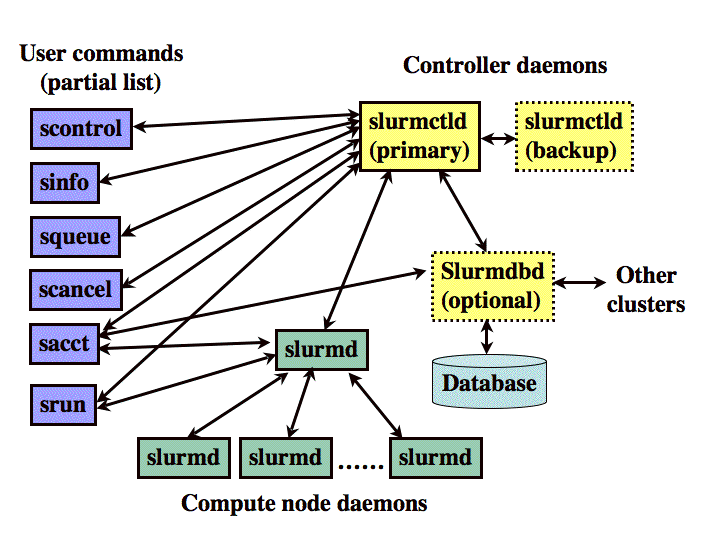
\includegraphics[width=15cm]{figuras/archSingularity.png}}
\caption{Arquitectura de Slurm}
\medskip
\small
\centerline{Fonte: \url{https://slurm.schedmd.com/quickstart.html}}
\end{figure}

A arquitectura do xestor de recursos Slurm pode ser apreciada na figura \ref{archSingularity}. Se o lector desexa ampliar os seus coñecementos acerca do mesmo, pode consultar a documentación oficial\footnote{\url{https://slurm.schedmd.com/}}.

\section{Alternativas: \gls{MV}s fronte a contedores}

A necesidade de crear entornos illados e portábeis non se trata de ningunha novidade. As máquinas virtuais xa introduciron hai tempo esta idea, coa posibilidade de incluír no seu interior todas as dependencias software precisas, librarías, código e datos, para seren executadas en calquera lugar.\\

As \gls{MV}s permiten a creación de entornos completamente illados, facendo segura a outorga de privilexios de superusuario no seu interior aos usuarios. As \gls{MV}s posúen un sistema operativo completo, incluíndo unha propia administración da memoria e a emprega de controladores para dispositivos virtuais. Debido ao uso que fai do hipervisor, este impide que unha \gls{MV} poida executar instrucións que poñan en risco a integridade da máquina anfitrioa \cite{introduccionContainerSecurityDocker}. Non obstante, este illamento tamén engade complexidades adicionais cando tentamos que os entornos contidos no interior das \gls{MV} fagan uso de recursos propios da máquina anfitrioa, como poden ser redes escalábeis como InfiniBand, aceleradores hardware \cite{singularityScientificContainers} ou unidades de procesamento gráfico para computación paralela, recursos amplamente empregados en centros de supercomputación.\\

Coa incorporación de funcións de virtualización lixeiras para o \textit{kernel} de GNU/Linux, por exemplo, coa implantación dos espazos de nomes, foi posíbel implantar unha nova forma de virtualización: a virtualización a nivel de sistema operativo, tamén coñecida como contedores. Este tipo de virtualización presenta a gran vantaxe fronte ás \gls{MV}s que poden compartir unha serie de recursos coa máquina anfitrioa, supondo unha penalización de rendemento moi pequena e en case calquera caso desprezábel. Dito funcionamento fai que os contedores sexan máis lixeiros, rápidos e doados de escalar que as \gls{MV}s, permitindo un funcionamento moito máis flexíbel \cite{introduccionContainerSecurityDocker}. Deste xeito, os contedores permitiron a creación de entornos personalizábeis polo usuario cunha perda de mínima de rendemento, pondo solución ao complexo problema de dependencias software.\\

Podemos concluír que ambos, contedores e \gls{MV}s, provén entornos illados para a execución de aplicacións baixo unha máquina anfitrioa compartida, pero baixo perspectivas técnicas ben distintas. Estas solucións poden ser empregadas de forma independente ou en conxunto, dependendo das necesidades do entorno. Por exemplo, unha boa solución de compromiso entre seguridade e utilidade podería pasar polo despregamento de contedores dentro de \gls{MV}s. Este enfoque aumenta a seguridade ao introducir dúas capas de virtualización, as \gls{MV}s e os contedores, ademais de ofertar os beneficios de despregamento rápido outorgados polos contedores. Polo tanto, pódese acadar un illamento de aplicacións máis sólido combinando a virtualización mediante \gls{MV}s e a contedorización. A figura \ref{CombinacionVirtualizacion} amosa unha representación gráfica de dita implantación. Non obstante, existen certos escenarios que poden non ser bos candidatos para a emprega de \gls{MV}s e nos que no seu canto, o uso de contedores supón unha mellor solución. Por exemplo, aplicacións de rendemento crítico ou aplicacións que fagan uso de hardware especializado no que sexa preciso un acceso directo ao mesmo, supondo neste caso un problema os beneficios do alto illamento dado polas \gls{MV}s. Este é o caso dos centros de supercomputación, como pode ser o \gls{CESGA}, por exemplo, coa execución de aplicacións de procesamento paralelo que fagan uso da \gls{GPU}.

\begin{figure}
\centerline{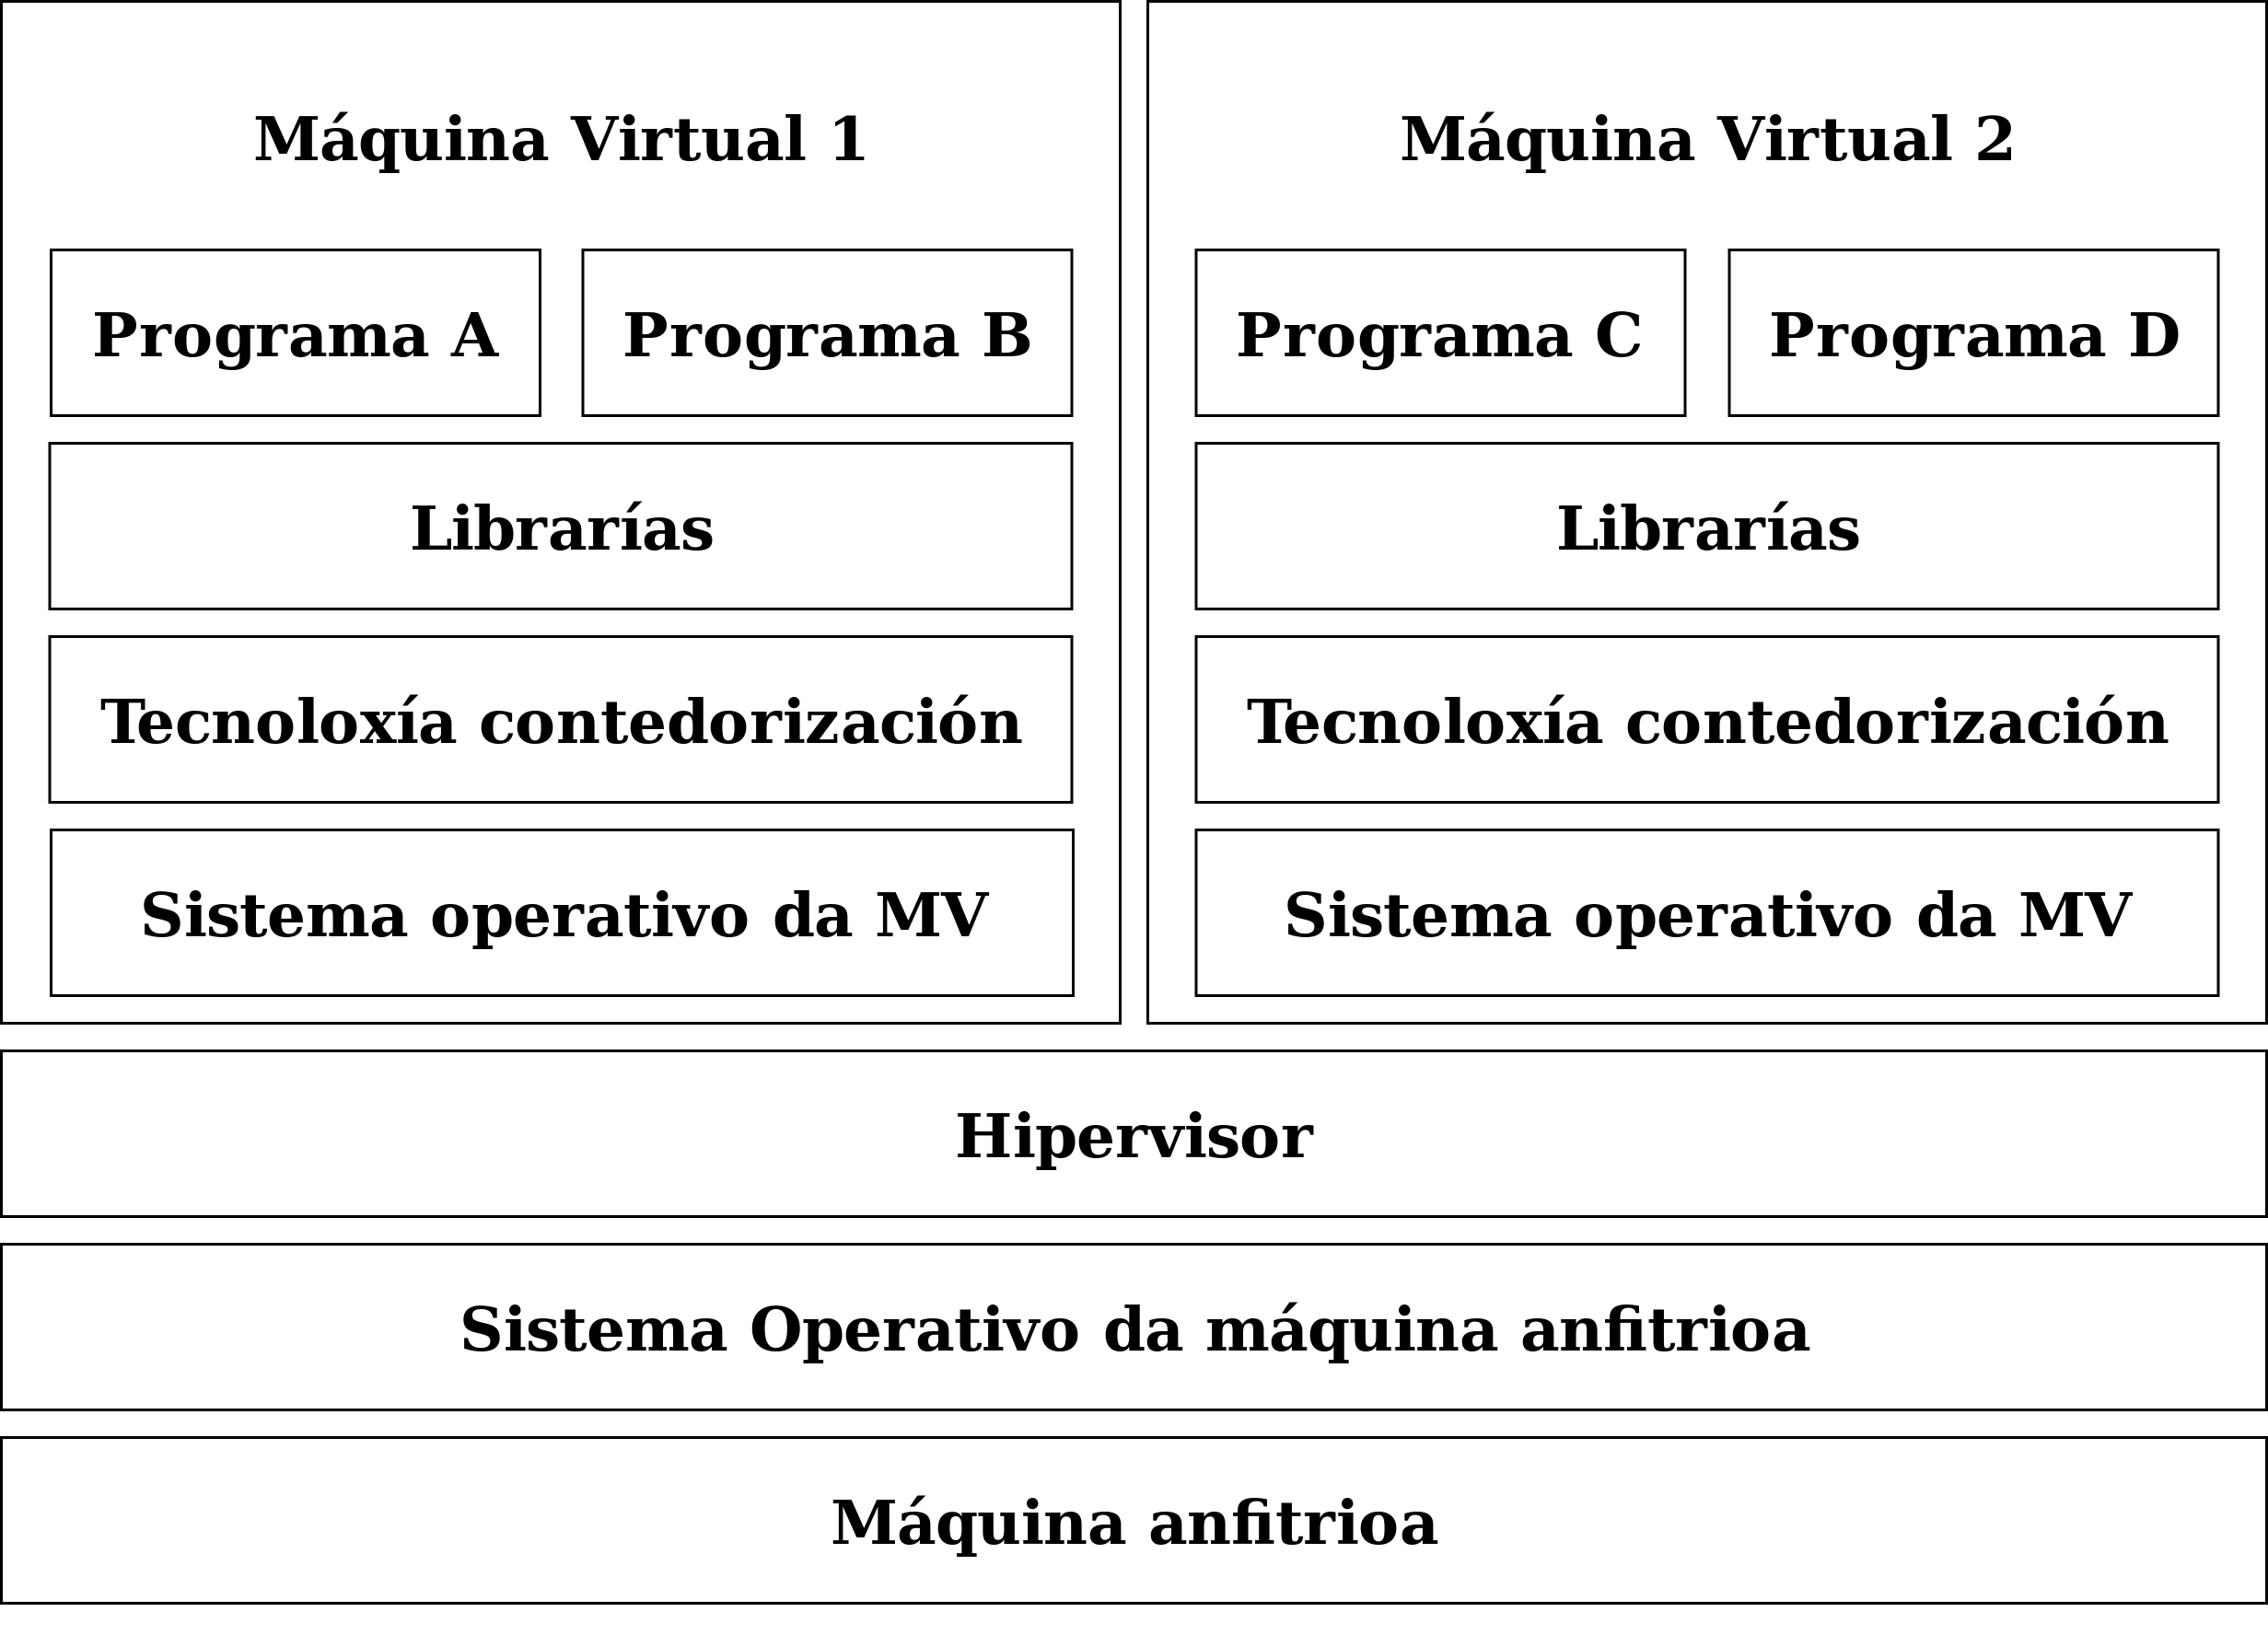
\includegraphics[width=15cm]{figuras/CombinacionVirtualizacion.png}}
\caption{Combinación das tecnoloxías de virtualización}
\label{CombinacionVirtualizacion}
\end{figure}

\section{Computación na nube no \gls{CESGA}}

A computación na nube (ou \textit{Cloud Computing}) é un paradigma que permite ofertar servizos de computación a través dunha rede, habitualmente Internet. O \gls{CESGA} dispón un servizo de computación na nube no cal é posíbel entregar aos usuarios unha infraestrutura de computación virtual e configurábel á medida e requisitos do usuario final: sistema operativo, número de procesadores, memoria, disco e número de nodos son determinados á medida do usuario de forma dinámica. Para a xestión do sistema utilízase o software OpenNebula\footnote{\url{https://opennebula.org/}}. \cite{CloudCESGA}\\

Posto que non todas as probas poderán ser feitas directamente sobre contedores correndo no \gls{FT2}, motivado principalmente pola falta de permisos de execución, farase uso dos servizos de computación na nube para despregar máquinas virtuais sobre as cales poder configurar todos os requirimentos necesarios.

\section{Conclusións}

A diversidade existente na comunidade que fai uso destes recursos de computación de altas prestacións provoca que os centros \gls{HPC} deban manter sistemas estábeis, fiábeis e funcionais, o que moitas veces implica a conserva de sistemas en versións antigas e xa amplamente testadas. No entanto, hoxe en día, a integración continua, as metodoloxías de desenvolvemento áxiles e os lanzamentos continuos (\textit{rolling realeases}) son conceptos cada vez máis empregados no desenvolvemento do software científico. Posuír un software \gls{HPC} mantido ao día neste escenario e seguir a empregar integracións e despregamentos tradicionais, xunto sistemas non actualizados, supón un problema de engarrafamento. Unha das solucións máis flexíbeis e soadas nestes días podería pasar pola emprega de contedores. Polo tanto, podemos dicir que a necesidade á que dan resposta os contedores é ofertar unha maneira simple e eficiente que permita implantar e despregar este complexo software con todas as súas dependencias, sen perder a capacidade computacional dun sistema de \gls{HPC}. Porén, aínda que son moitos os beneficios aportados polos contedores, non debemos esquecer que posúen unha serie de características que fan que a súa seguridade teña que ser estudada con cautela. Ao longo deste documento estudaremos tales características.
\cleardoublepage
\chapter{Detección de vulnerabilidades en imaxes}
\minitoc
\clearpage

\section{Introdución}

Cando traballamos cun entorno baseado en contedores, debemos ter presente que, xunto con todas as vantaxes que estes aportan, como pode ser o despregamento de entornos áxiles, tamén estamos a introducir novos elementos no noso sistema que poden chegar a supor novos posíbeis vectores de ataque. A implicación de novos sistemas operativos e librarías no conxunto do novo sistema poden levar a aparición de novas vulnerabilidades que non poden ser tan doadamente controladas coma se estivésemos a tratar co noso sistema principal (a máquina anfitrioa). Este feito vén, precisamente, asociado á simplicidade de despregamento destes entornos.\\

Cabe a posibilidade de que un usuario, de xeito intencionado ou non, despregue un contedor con vulnerabilidades incluídas no seu interior e así supor unha punto de entrada para a posterior execución de \textit{malware}. Este feito vese agravado se temos en conta que o que se desexa facer é acadar un sistema multiusuario onde cada quen poida despregar os seus propios contedores. Para minimizar as posibilidades de que este fenómeno aconteza, é boa idea descargar e empregar soamente contedores obtidos de fontes fiábeis, das cales coñezamos o seu lexítimo creador.

\section{Portais de almacenamento de contedores}

Así, entran en xogo numerosos portais de almacenamento de contedores, como poden ser Docker Hub\footnote{\url{https://hub.docker.com/}} ou Singularity Hub\footnote{\url{https://singularity-hub.org/}}. Ditos portais poden amosarnos información útil para comprender as implicacións de seguridade que pode ter a emprega das imaxes dos contedores aí almacenados. Por exemplo, en primeiro lugar identificarase o autor de dito contido, dándonos a coñecer se se trata de material oficial, ou provinte ou non dunha fonte da nosa confianza. Ademais, os portais poden contar con medidas máis avanzadas no referente á seguridade, que permitan un maior coñecemento do que estamos a descargar. Para aclarar a hipótese exposta, mostrarase un exemplo sobre unha das plataformas previamente nomeadas.\\

Mais antes de comezar con dito exemplo, cómpre ter un par de termos claros: un contedor é lanzado cando corremos unha imaxe. Polo tanto, unha imaxe constitúe un paquete executábel que inclúe todo o necesario para correr unha aplicación (código, librarías, variábeis de entorno, ficheiros de configuración...). Pola contra, un contedor é a instancia en tempo de execución dunha imaxe, é dicir, no que a imaxe se transforma na memoria cando é executada. \cite{docker-get-started}\\

\subsection[Exemplo práctico: Docker Hub]{Exemplo práctico: estudo das medidas avanzadas de seguridade nunha plataforma de almacenamento: Docker Hub}

\subsubsection{Introdución}

O Docker Hub trátase dun servizo baseado na nube para o rexistro de contedores, así como permitir construír imaxes e probalas. Tamén constitúe un recurso centralizado para o descubrimento, distribución, xestión de cambios e automatización do fluxo de traballo en toda a liña de desenvolvemento. \cite{dockerHubExp}\\

Este servizo permítenos procurar entre multitude de imaxes, a través das cales podemos obter sistemas completamente configurados para o seu despregamento e posta en marcha. Outra característica a ter en conta é que as novas imaxes non teñen por que ser refeitas de cero, senón que é posíbel estender imaxes xa existentes, habendo así unha relación pai-fillo entre imaxes e podendo facer ramas doutros repositorios. Concretando un pouco máis, cada imaxe de Docker está composta por unha lista de capas de só lectura. Na máquina anfitrioa, cada capa será almacenada coma un ficheiro \textit{tar} cun único directorio. As capas son empilladas xerarquicamente, onde o seu orde queda especificado nun ficheiro \gls{JSON} de configuración  \cite{studySecurityDockerHub}. Polo tanto, parte destas capas poden ser reempregadas integramente cando creamos unha nova imaxe en base a outra xa existente.

\subsubsection{Fontes}

Cando descargamos estes contedores debemos prestar especial atención á súa orixe. Deste xeito, a plataforma permítenos distinguir entre contedores oficiais, que son aqueles provintes dos propios desenvolvedores dunha tecnoloxía; e entre repositorios públicos dun determinado autor. Os repositorios oficiais son considerados de maior confianza, posto que son dados polos propios creadores da tecnoloxía, e son sometidos a probas de seguridade por parte do Docker Hub, namentres que os repositorios públicos doutros usuarios simplemente poden ser descargados, pero as súas medidas previas de seguridade son moito máis limitadas.\\

\begin{figure}
\centerline{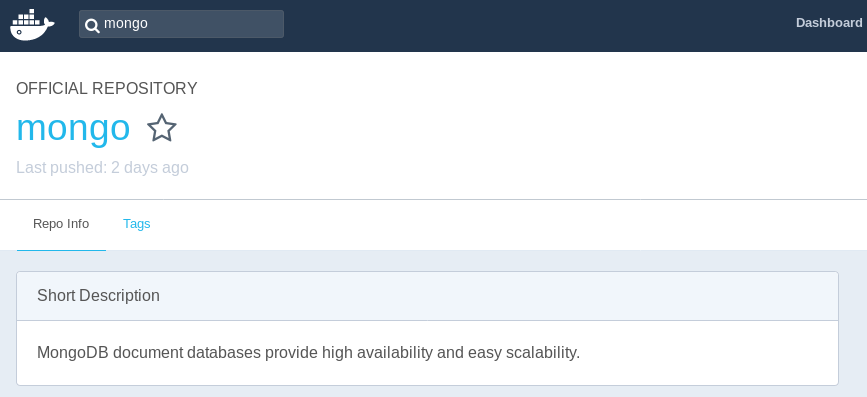
\includegraphics[width=15cm]{figuras/dockerOficial}}
\caption{Exemplo dun repositorio oficial no Docker Hub.}
\label{dockerOficial}
\end{figure}

\begin{figure}
\centerline{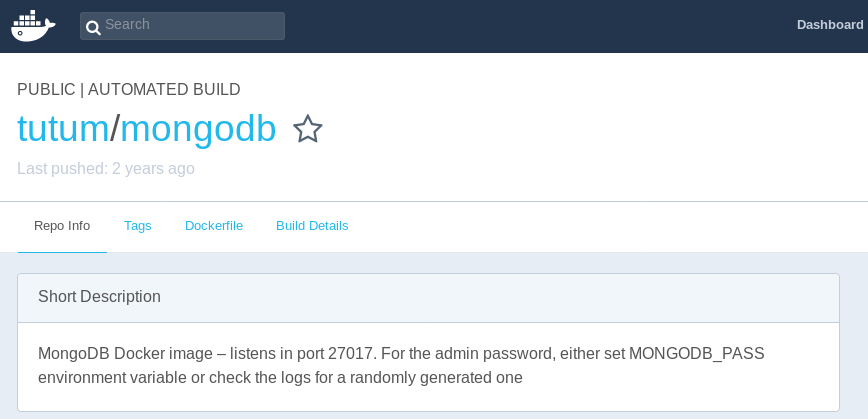
\includegraphics[width=15cm]{figuras/mongoNonOficial.png}}
\caption{Exemplo dun repositorio non oficial no Docker Hub.}
\label{mongoNonOficial}
\end{figure}

Na figura \ref{dockerOficial} pódese observar a aparición da frase ``\textit{Official repository}'', indicando que o repositorio en cuestión provén dunha fonte fiábel, mentres que na figura \ref{mongoNonOficial} pódese ver como se trata dun repositorio público, pero que non provén de fontes oficiais, senón dun usuario concreto.

\subsubsection{Medidas estendidas de seguridade}

O Docker Hub oferta medidas estendidas de seguridade para os repositorios de fontes oficiais, como son a identificación e clasificación de vulnerabilidades segundo o seu nivel de risco. Por exemplo, se consultamos a etiqueta (\textit{tag}) correspondente á derradeira versión considerada estábel do \gls{SXBD} MongoDB\footnote{\url{https://www.mongodb.com/}} (\textit{3.6.4-jessie} arestora), podemos observar como o Docker Hub indícanos a aparición dun total de 13 compoñentes vulnerábeis, entre os 102 que conforman a imaxe. Amais, estes compoñentes son analizados segundo a capa á que pertenzan e clasificados segundo o seu nivel de risco. Esta información pode ser consultada na figura \ref{mongoOficialVulnerabilidades}, e non se trata de información meramente cuantitativa, senón que tamén se indican explicitamente as vulnerabilidades atopadas e a fonte, tal e como pode ser observado na figura \ref{mongoOficialVulnerabilidades2}. Por exemplo, é posíbel observar como este repositorio posúe vulnerabilidades consideradas de nivel crítico asociadas á libraría {\it glibc 2.19-18+deb8u10}.\\

\begin{figure}
\centerline{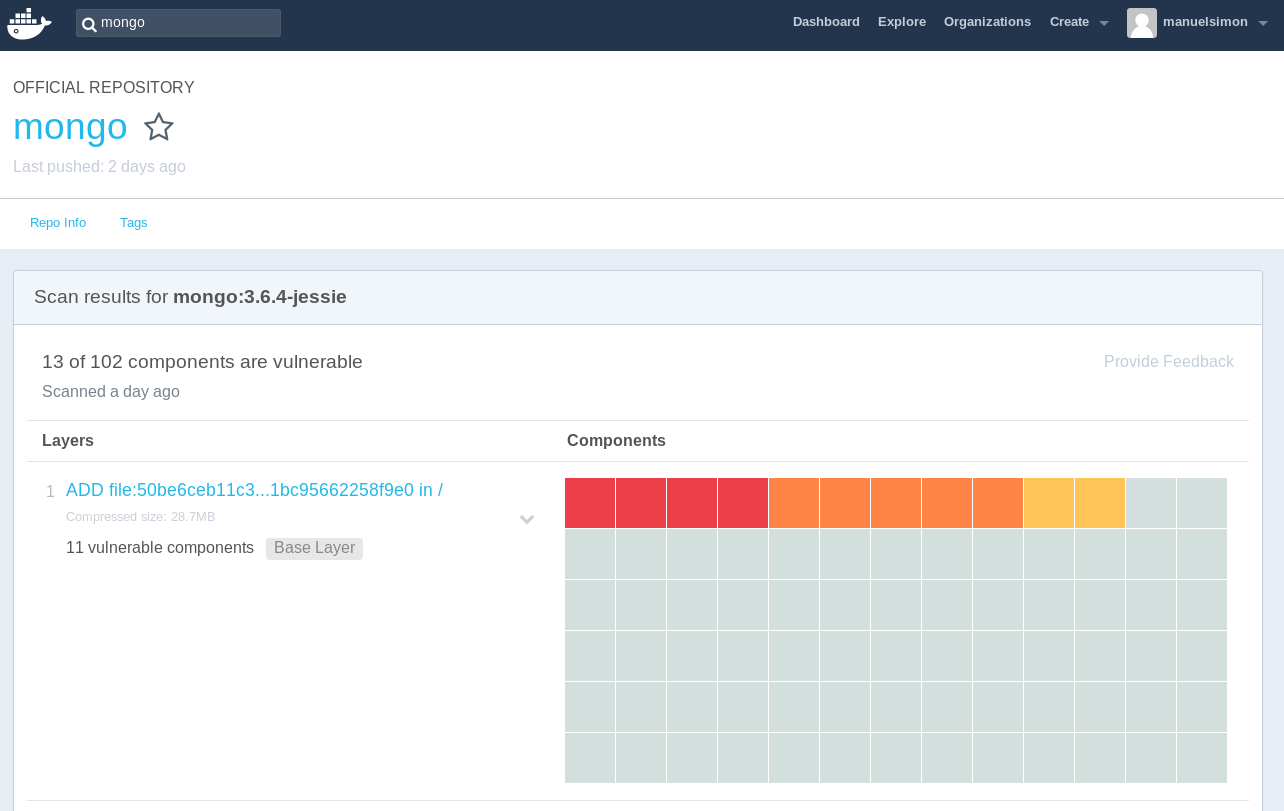
\includegraphics[width=15cm]{figuras/mongoOficialVulnerabilidades.png}}
\caption{Vulnerabilidades atopadas nun contedor oficial no Docker Hub. Parte 1.}
\label{mongoOficialVulnerabilidades}
\end{figure}

\begin{figure}
\centerline{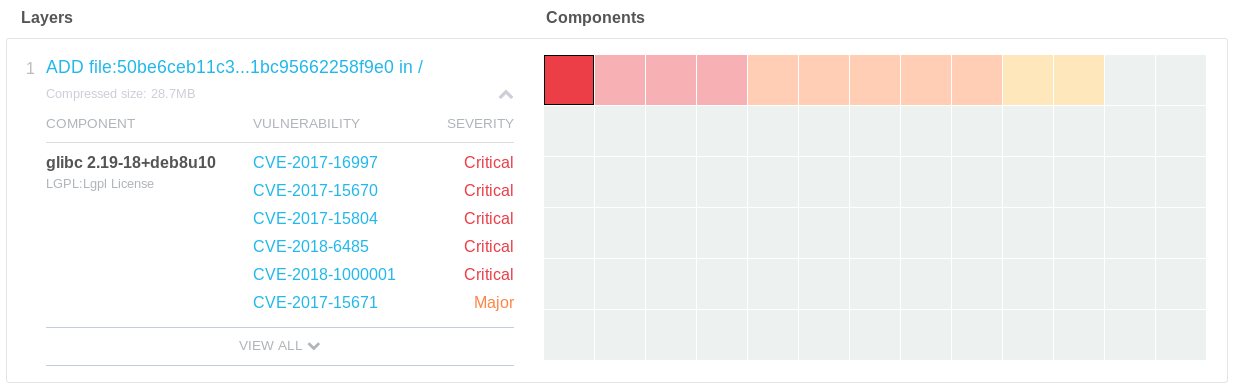
\includegraphics[width=15cm]{figuras/mongoOficialVulnerabilidades2.png}}
\caption{Vulnerabilidades atopadas nun contedor oficial no Docker Hub. Parte 2.}
\label{mongoOficialVulnerabilidades2}
\end{figure}

Este tipo de vulnerabilidades serán máis doadas de atopar canto máis complexa sexa a imaxe do contedor a montar, polo que é importante procurar seguir o principio da máxima simplicidade posíbel, empregando sempre un conxunto de contedores o máis simples que poidamos. Por exemplo, se consultamos no Docker Hub o repositorio dun \textit{Hello World}, podemos ver como non presenta ningún tipo de vulnerabilidade coñecida até o momento, tal e como ser apreciado nas figuras \ref{helloWorldSenVulnerabilidades} e \ref{helloWorldSenVulnerabilidades2}.

\begin{figure}
\centerline{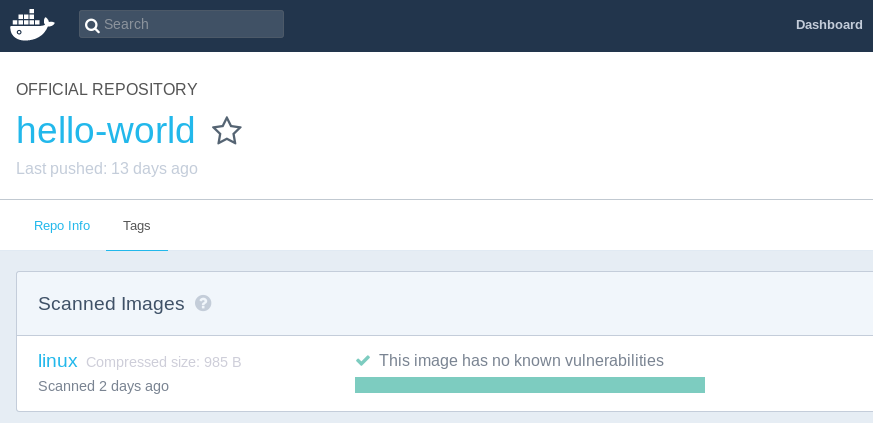
\includegraphics[width=15cm]{figuras/helloWorldSenVulnerabilidades.png}}
\caption{Repositorio \textit{Hello World} sen vulnerabilidades atopadas. Parte 1.}
\label{helloWorldSenVulnerabilidades}
\end{figure}

\begin{figure}
\centerline{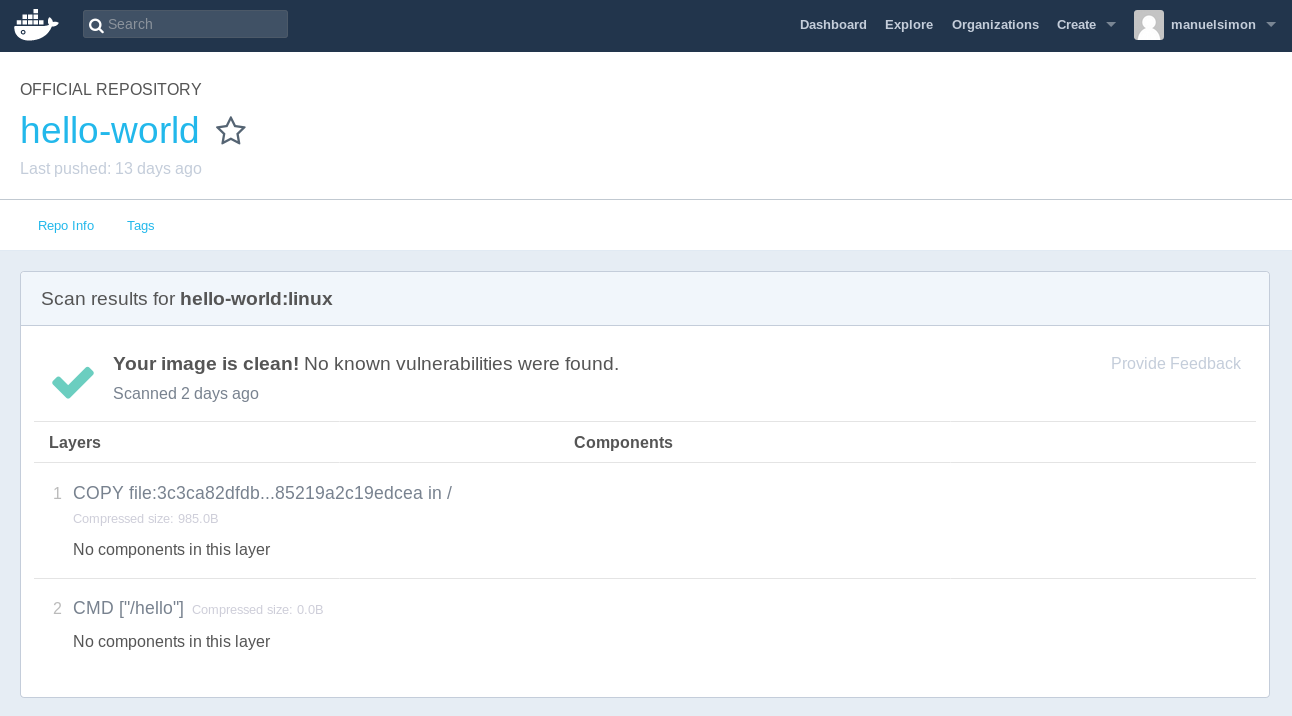
\includegraphics[width=15cm]{figuras/helloWorldSenVulnerabilidades2.png}}
\caption{Repositorio \textit{Hello World} sen vulnerabilidades atopadas. Parte 2.}
\label{helloWorldSenVulnerabilidades2}
\end{figure}

\subsubsection{Conclusións}

Polo tanto, endexamais debemos asumir que polo feito de estaren incluídos nun directorio centralizado, como pode ser o Docker Hub, os contedores están libres de vulnerabilidades. Deberiamos empregar contedores cuxas fontes, desenvolvedores ou repositorios sexan coñecidos e considerados de confianza, e na medida do posíbel, empregar soamente aqueles mantidos por unha fonte oficial ou comunidade.

\section{Herdanza de vulnerabilidades}

Continuando coa idea anteriormente presentada da posíbel dependencia entre imaxes mediante as relacións pai-fillo, dende o punto de vista da seguridade informática é importante remarcar que, aínda que esta é unha característica moi útil para reducir custos e engadir flexibilidade, coa dependencia entre imaxes tamén se probará calquera vulnerabilidade de software que a imaxe pai contivese se non son aplicadas as medidas e actualizacións de seguridade precisas \cite{studySecurityDockerHub}. Moitas veces, estas medidas pasan por simplemente actualizar as librarías no interior do contedor á súa última versión (por exemplo, aplicando un {\tt apt-get update \&\& apt-get upgrade}). A importancia de manter o sistema actualizado quedará representada na sección \ref{actualizacionSistema}. Asemade, evidenciando os riscos de seguridade que implican estas dependencias entre imaxes, Rui Shu, Xiaohui Gu e William Enck levaron a cabo un estudo (``\textit{A Study of Security Vulnerabilities on Docker Hub}'' \cite{studySecurityDockerHub}) no que realizaron múltiples análises e entre as cales podemos atopar un exemplo de herdanza de vulnerabilidades entre imaxes dependentes. Este exemplo pode ser contemplado na figura \ref{herdanzaVulnerabilidades}.

\begin{figure}
\centerline{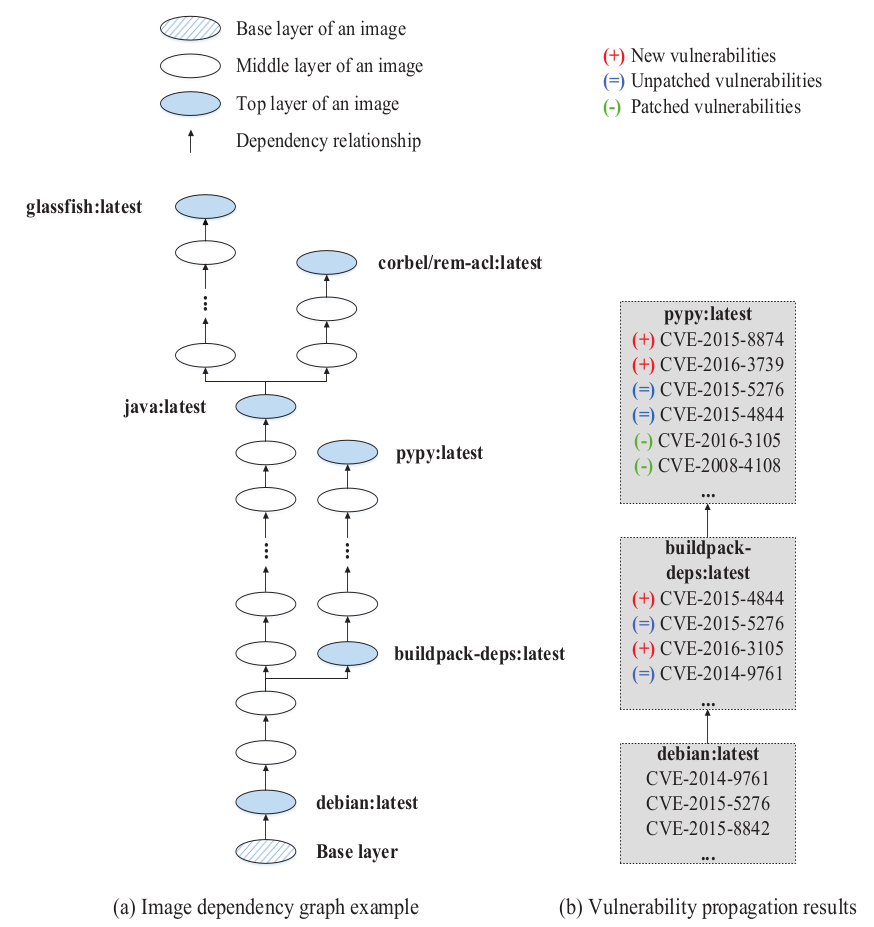
\includegraphics[width=15cm]{figuras/herdanzaVulnerabilidades.png}}
\caption{Exemplo de herdanza de vulnerabilidades}
\medskip
\small
\centerline{Fonte: \cite{studySecurityDockerHub}}
\label{herdanzaVulnerabilidades}
\end{figure}

\section{Detección de vulnerabilidades con Clair}

\subsection{Necesidade da ferramenta}

Os contedores poden incluír vulnerabilidades xa coñecidas no seu interior, tendo importantes implicacións de seguridade. Para evitar expor o noso sistema é importante ter coñecemento das posíbeis consecuencias que pode traer o despregamento de certo contedor. Aínda que algúns rexistros de imaxes, como pode ser o Docker Hub, xa inclúen mecanismos para informarnos acerca das vulnerabilidades atopadas en certas imaxes, non sempre faremos uso de fontes con mecanismos de seguridade tan avanzados, senón que é posíbel que cheguen contedores de múltiples fontes das que non será tan sinxelo obter unha información tan detallada. Ademais, tamén cabe a posibilidade de que tras facer cambios no contedor, tivésemos creado sen sabelo un entorno que inclúe vulnerabilidades. Debido a estes feitos, cómpre aplicar políticas propias de detección de vulnerabilidades en imaxes previo ao seu despregamento como contedores no entorno ou antes de proseguir cun proceso de integración continua.\\

Unha alternativa para realizar unha análise dos contedores pode tratarse do proxecto de código aberto Clair, o cal realiza unha análise estática de vulnerabilidades en contedores. Actualmente inclúe suporte para contedores Docker e appc \cite{clair}, pero existen adaptacións para a análise de contedores propios de Singularity.

\subsection{Funcionamento}

Esta ferramenta extraerá información tal como: 1) a versión dos paquetes de software instalados ou 2) os metadatos do sistema operativo en cada unha das capas que conforman a imaxe. A información detallada pode ser consultada na táboa \ref{datosClair}.\\

\begin{table}[]
\centering
\caption{Datos recollidos por Clair}
\label{datosClair}
\resizebox{\textwidth}{!}{%
\begin{tabular}{|c|c|}
\hline
\textbf{Nome do campo} & \textbf{Descrición}\\ \hline
\textit{Timestamp} & Data exacta do análise \\ \hline
ID da vulnerabilidade & Identificador unívoco da vulnerabilidade no \gls{CVE}\\ \hline
Nivel de gravidade & Clasificación da gravidade da vulnerabilidade\\ \hline
Descrición do \gls{CVE} & Descrición de cada vulnerabilidade identificada\\ \hline
Paquetes asociados & Nome e versión exacta dos paquetes vulnerábeis\\ \hline
Identificador da capa & Indicador da capa onde reside a vulnerabilidade atopada\\ \hline
\end{tabular}
}
\end{table}

Os datos sobre vulnerabilidades son importados continuamente dende un conxunto coñecido de fontes e son correlacionados cos contidos indexados das imaxes dos contedores para xerar listas de vulnerabilidades que poñen en risco aos mesmos \cite{clairWeb}. Clair identifica os paquetes inseguros realizando emparellamentos entre os metadatos e as listas de vulnerabilidades coñecidas (\gls{CVE}s). Cabe destacar que Clair soamente indentifica a presenza de paquetes con vulnerabilidades coñecidas; non determina se eses paquetes van ser empregados verdadeiramente, nin tampouco existe a posibilidade de detectar un comportamento dinámico nos contedores unha vez instanciados (por exemplo, novos paquetes vulnerábeis poderían ser instalados nos contedores en execución). \cite{studySecurityDockerHub} \\

Clair pode ser integrado directamente cun rexistro de contedores, automatizando o escaneo de imaxes e establecendo un mecanismo seguro para a notificación de vulnerabilidades, o que permitirá fornecer a seguridade do noso sistema. A arquitectura final desta ferramenta quedaría entón conformada por unhas fontes fiábeis de vulnerabilidades coñecidas, das que se obtería a información para ser gardada nunha base de datos relacional xestionada polo \gls{SXBD} PostgreSQL\footnote{\url{https://www.postgresql.org/}}, o nomeado rexistro de imaxes e, finalmente, un punto final de notificación das vulnerabilidades atopadas. Dita arquitectura está representada na figura \ref{clair-diagram}.

\begin{figure}
\centerline{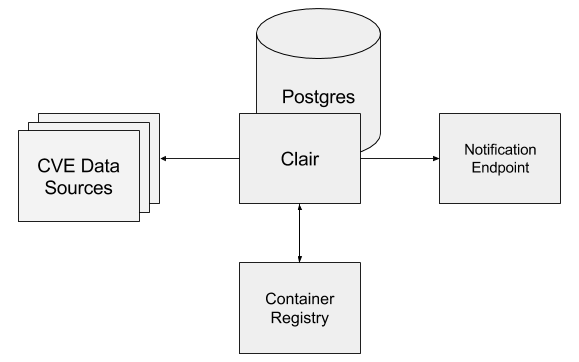
\includegraphics[width=15cm]{figuras/clair-diagram.png}}
\caption{Arquitectura de Clair}
\small
\centerline{Fonte: \url{https://github.com/coreos/clair/blob/master/Documentation/running-clair.md}}
\label{clair-diagram}
\end{figure}

\subsection{Probas}

Nesta sección serán realizadas unha serie de probas para amosar o funcionamento da ferramenta Clair, así como para deixar patentes os riscos asociados á emprega de imaxes sen ter coñecemento das vulnerabilidades existentes nas mesmas.

\subsubsection{Docker}
\label{clairScannerDocker}

Para o estudo con contedores Docker, empregarase a ferramenta {\it clair-scanner} \footnote{\url{https://github.com/arminc/clair-scanner}}, a cal permite unha análise das vulnerabilidades das imaxes gardadas na propia máquina local. É dicir, rediriximos o rexistro á propia máquina local, simplificando a arquitectura habitual de Clair amosada na figura \ref{clair-diagram}. Os motivos que impulsan esta simplificación vén dados por: 1) estase a traballar cunha proba de concepto, 2) Clair non está implantado actualmente no sistema do \gls{FT2} e 3) a súa implantación non ten sentido actualmente, ao non existir tampouco soporte para Docker. Esta ferramenta tamén presenta a posibilidade de comparar as vulnerabilidades atopadas cunha lista branca, na cal é posíbel indicar vulnerabilidades que pasaremos por alto se fose a nosa vontade, acadando de tal xeito un alto nivel de flexibilidade. Posto que estamos a substituír o rexistro por imaxes atopadas na propia máquina local, esta proba non suporá un método automatizado de análise de imaxes como o que Clair pode chegar a acadar. No entanto, xa que non existe actualmente un rexistro de contedores no \gls{CESGA}, a proba a realizar exemplificará perfectamente o funcionamento de Clair sen precisar deste compoñente.\\

O proceso de emprega de Clair pasaría polas seguintes fases:

\begin{enumerate}
    \item Un desenvolvedor de software obtén unha imaxe ou crea o seu contedor e envía unha imaxe do mesmo a Clair.
    \item Clair analiza a imaxe, na procura de vulnerabilidades de seguridade.
    \item Clair devolve un informe detallado das vulnerabilidades de seguridade atopadas na imaxe.
    \item O desenvolvedor actúa en base ao informe.
        \begin{itemize}
            \item Procura unha solución alternativa solucionando as vulnerabilidades.
            \item Con coñecemento da súa existencia, asume os riscos asociados ás vulnerabilidades e adiciona as mesmas á lista branca.
        \end{itemize}
\end{enumerate}

A análise mediante a nomeada ferramenta efectúase seguindo os seguintes comandos:

\begin{lstlisting}[,caption={Análise de imaxes de contedores mediante \textit{clair-scanner}}]
docker run -p 5432:5432 -d --name db arminc/clair-db:`date -d "-2 day" '+%Y-%m-%d'`
docker run -p 6060:6060 --link db:postgres -d --name clair arminc/clair-local-scan:v2.0.1
clair-scanner --ip 172.17.0.1 $IMAGEID
\end{lstlisting}

\begin{figure}
\centerline{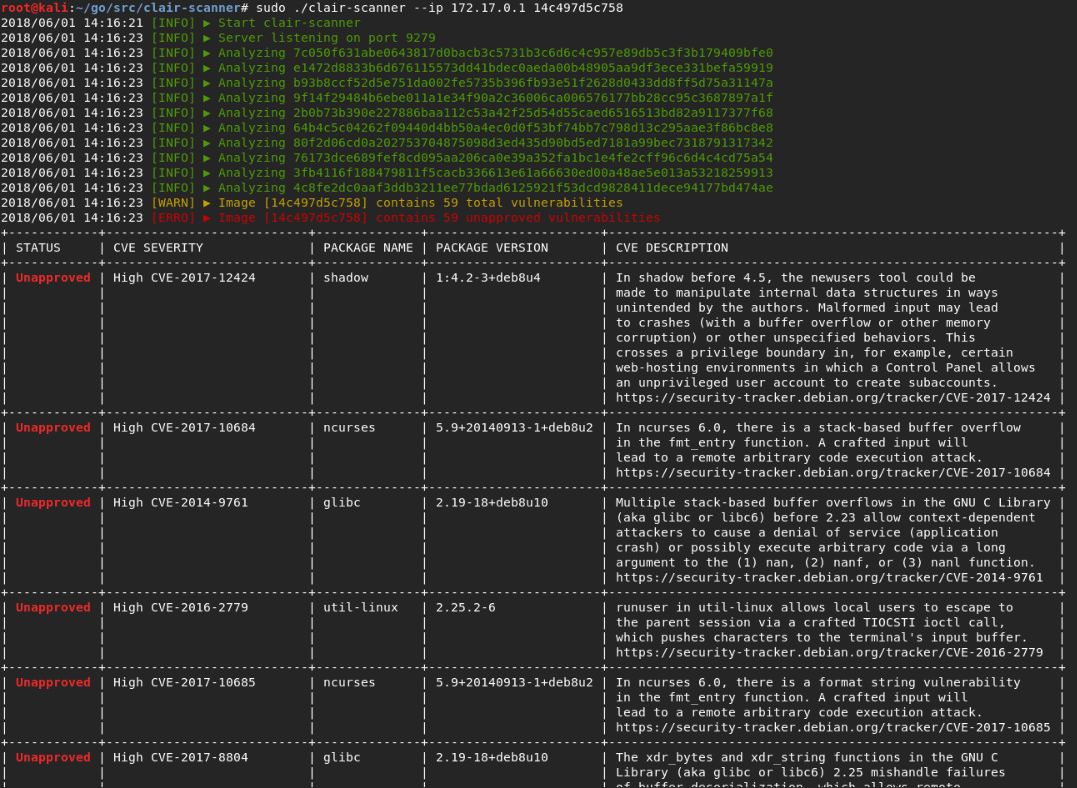
\includegraphics[width=15cm]{figuras/clairDocker.png}}
\caption{Exemplo de execución de {\it clair-scanner}}
\label{clairDocker}
\end{figure}

Isto equivalería a despregar un contedor coa base de datos de vulnerabilidades actualizada e outro contedor coa ferramenta Clair. Finalmente invocamos ao {\it clair-scanner} e amósanos os resultados das vulnerabilidades atopadas sobre a imaxe, tal e como pódese ver na figura \ref{clairDocker}.

\subsubsection{Singularity}

Existe unha adaptación de Clair para traballar sobre contedores Singularity\footnote{\url{https://github.com/dctrud/clair-singularity}}. O seu funcionamento baséase no feito de que un arquivo \textit{.tar.gz} exportado dunha imaxe Singularity é similar a unha imaxe dunha única capa dun contedor Docker. Polo tanto, esta ferramenta:

\begin{enumerate}
    \item Exporta unha imaxe Singularity a un arquivo temporal \textit{.tar.gz}.
    \item Calcula o \textit{hash} \gls{SHA}-256 como nome único a dar a Clair.
    \item Envía o arquivo \textit{.tar.gz} a través dun servidor \gls{HTTP} incorporado, mediante o cal Clair pode recuperalo.
    \item Chama á \gls{API} de Clair para que analice o arquivo \textit{.tar.gz} como unha capa para o análise.
    \item Chama á \gls{API} de Clair para o obter o informe de vulnerabilidades.
    \item Amosa os resultados por pantalla.
\end{enumerate}

Dita ferramenta aínda non posúe soporte para certificados de cliente \gls{SSL}, polo que non é posíbel verificar que estamos a enviar solicitudes a unha instancia Clair fiábel. Polo tanto, dita solución resulta insegura a non ser que a empreguemos baixo un entorno illado local. Este tipo de entorno foi o escollido para desenvolver as probas que se amosan a continuación.

\begin{lstlisting}[,caption={Análise dunha imaxe \textit{Hello-World} Singularity}]
bash-4.3# singularity build hello-world.simg docker://hello-world
Docker image path: index.docker.io/library/hello-world:latest
Cache folder set to /root/.singularity/docker
[1/1] |===================================| 100.0% 
Importing: base Singularity environment
Importing: /root/.singularity/docker/sha256:9bb5a5d4561a5511fa7f80718617e67cf2ed2e6cdcd02e31be111a8d0ac4d6b7.tar.gz
Importing: /root/.singularity/metadata/sha256:942999de4612d732c9e2b49bcd0633781edd5f3bd457d5f4f6cdc965b1abef9e.tar.gz
Building Singularity image...
Singularity container built: hello-world.simg
Cleaning up...

bash-4.3# sclair hello-world.simg 
Found 27 Clair namespaces
Clair URL: http://127.0.0.1:6060/v1

1. Starting server...
======== Running on http://127.0.0.1:8080 ========
(Press CTRL+C to quit)

1. Checking server...
2. Processing images!
Exporting hello-world.simg to targz...
2.4.5-dist
...exported hello-world.simg to /tmp/tmpo39pub_w/singularity-clair.d1hbbu74.tar.gz
...serving http://127.0.0.1:8080/images/singularity-clair.d1hbbu74.tar.gz to Clair
3. Generating report!
hello-world.simg does not have any vulnerabilities!
\end{lstlisting}

Como pode ser apreciado no código anterior, unha imaxe Docker é descargada dende o repositorio do Docker Hub e é adaptada a Singularity, grazas aos servizos de importación cos que conta esta tecnoloxía de contedorización. Posteriormente é analizada pola adaptación da ferramenta Clair para imaxes Singularity. Rematado o escáner, é posíbel apreciar como esta imaxe non presenta ningunha vulnerabilidade coñecida, tal e como xa puideramos ollar no repositorio do Docker Hub de onde provén, ao ser unha imaxe moi simple.\\

Seguindo o mesmo procedemento que no caso anterior, o Clair analizou nunha nova execución unha imaxe adaptada a Singularity correspondente ao Mongo DB, na súa versión \textit{3.6.4-jessie}. Como amosan os resultados, esta imaxe si que presenta vulnerabilidades coñecidas.

\begin{lstlisting}[,caption={Análise dunha imaxe MongoDB Singularity}]
bash-4.3# singularity build mongo.simg docker://mongo:3.6.4-jessie
Docker image path: index.docker.io/library/mongo:3.6.4-jessie
Cache folder set to /root/.singularity/docker
[10/10] |===================================| 100.0% 
Importing: base Singularity environment
Importing: /root/.singularity/docker/sha256:4d0d76e05f3c6caf923a71ca3b3d2cc8c834ca61779ae6b6d83547f3dd814980.tar.gz
.
.
.
Importing: /root/.singularity/metadata/sha256:2087064d2efc26145ab24e8a245e92d56e97c9e6df934621d02524aab46bea19.tar.gz
Building Singularity image...
Singularity container built: mongo.simg
Cleaning up...

bash-4.3# sclair mongo.simg 

Found 27 Clair namespaces
Clair URL: http://127.0.0.1:6060/v1

1. Starting server...
======== Running on http://127.0.0.1:8080 ========
(Press CTRL+C to quit)

1. Checking server...
2. Processing images!
Exporting mongo.simg to targz...
2.4.5-dist
...exported mongo.simg to /tmp/tmpvds_0eom/singularity-clair.k964yxz7.tar.gz
...serving http://127.0.0.1:8080/images/singularity-clair.k964yxz7.tar.gz to Clair
3. Generating report!
gnupg - 1.4.18-7+deb8u4
-----------------------
CVE-2018-6829 (Negligible)
https://security-tracker.debian.org/tracker/CVE-2018-6829
cipher/elgamal.c in Libgcrypt through 1.8.2, when used to encrypt messages directly, improperly encodes plaintexts, which allows attackers to obtain sensitive information by reading ciphertext data (i.e., it does not have semantic security in face of a ciphertext-only attack). The Decisional Diffie-Hellman (DDH) assumption does not hold for Libgcrypt's ElGamal implementation.


shadow - 1:4.2-3+deb8u4
-----------------------
CVE-2017-12424 (High)
https://security-tracker.debian.org/tracker/CVE-2017-12424
In shadow before 4.5, the newusers tool could be made to manipulate internal data structures in ways unintended by the authors. Malformed input may lead to crashes (with a buffer overflow or other memory corruption) or other unspecified behaviors. This crosses a privilege boundary in, for example, certain web-hosting environments in which a Control Panel allows an unprivileged user account to create subaccounts.


CVE-2018-7169 (Medium)
https://security-tracker.debian.org/tracker/CVE-2018-7169
An issue was discovered in shadow 4.5. newgidmap (in shadow-utils) is setuid and allows an unprivileged user to be placed in a user namespace where setgroups(2) is permitted. This allows an attacker to remove themselves from a supplementary group, which may allow access to certain filesystem paths if the administrator has used "group blacklisting" (e.g., chmod g-rwx) to restrict access to paths. This flaw effectively reverts a security feature in the kernel (in particular, the /proc/self/setgroups knob) to prevent this sort of privilege escalation.


CVE-2007-5686 (Negligible)
https://security-tracker.debian.org/tracker/CVE-2007-5686
initscripts in rPath Linux 1 sets insecure permissions for the /var/log/btmp file, which allows local users to obtain sensitive information regarding authentication attempts.  NOTE: because sshd detects the insecure permissions and does not log certain events, this also prevents sshd from logging failed authentication attempts by remote attackers.
.
.
.
\end{lstlisting}

\subsubsection{Udocker}

Udocker emprega as mesmas imaxes de contedores que Docker, sendo completamente compatíbel con moitos dos aspectos desta tecnoloxía. Así, o estudo realizado coa ferramenta \textit{clair-scanner} na sección \ref{clairScannerDocker} sobre as imaxes de Docker é exportábel a esta tecnoloxía de contedorización.

\section{Conclusións}

Como foi visto ao longo deste capítulo, as imaxes que darán lugar aos contedores que conformarán parte do noso sistema non están en ningún momento libres de conter vulnerabilidades, algunhas pudendo chegar a ser consideradas críticas. O feito de que ditas imaxes estean almacenadas en repositorios como o Docker Hub, ou que incluso sexan cedidas polos seus propios desenvolvedores non impide que conteñan ditas vulnerabilidades.\\

Tamén foi vista a importancia de contar con unha ferramenta de análise de vulnerabilidades a nivel local e non depender de servizos externos, posto que a orixe das imaxes pode chegar a ser moi heteroxéneo.\\

Polo tanto, podemos concluír que cando tratamos con contedores, os riscos de seguridade xa veñen dados incluso antes de chegar a facer algo na nosa propia infraestrutura, ao empregar materiais de terceiros e incorporar numerosas librarías e dependencias novas no noso sistema. É importante contar cun sistema que permita coñecer as vulnerabilidades ás que estaremos expostos, de traballar con certas imaxes, de forma que poidamos solucionalas ou ben asumir os seus riscos, pero sempre dende o coñecemento da súa existencia.

\cleardoublepage
\chapter{Validación de imaxes}
\minitoc
\clearpage

\section{Introdución}

Un aspecto moi a ter en conta no tratamento con contedores é a súa portabilidade, podéndoos transportar entre diferentes sistemas. Esta característica ten serias implicacións de seguridade, xa que é vital preservar e comprobar que os datos atopados no interior da imaxe non resulten alterados por unha terceira persoa. Así, ao transferir datos entre sistemas en rede e tratar cun medio non fiábel, como o é a Internet, é esencial garantir aspectos como autenticación (o creador do contedor é quen di ser), integridade (a imaxe non se viu modificada durante a transmisión) e non repudio (o creador da imaxe non pode negar que é el). Referirémonos a esta serie de aspectos como a validación das imaxes.

\section{Docker}
\label{dockerContentTruste}

Para garantir a validación de imaxes, Docker provén da ferramenta Docker Content Trust. Dita ferramenta permite a emprega de firmas dixitais, permitindo unha verificación da integridade no lado do cliente e o coñecemento do autor de etiquetas específicas dunha imaxe. Non obstante, esta utilidade non está activada por defecto, polo que o entorno debe ser configurado para isto.

\begin{lstlisting}[,caption={Activación do Docker Content Trust}]
export DOCKER_CONTENT_TRUST=1
\end{lstlisting}

As firmas dixitais son realizadas sobre as etiquetas, polo que é posíbel que existan etiquetas firmadas dunha imaxe e outras que non, sendo elección do autor se firmar unha etiqueta específica ou non. De cara ao usuario, este só poderá traballar con imaxes que estean firmadas, quedando inhabilitadas todas aquelas imaxes ou etiquetas que non o estivesen.\\

Para este control existen unha serie de chaves, que son creadas cando se invoca por primeira vez unha operación deste sistema de aseguranza da integridade. Este conxunto de chaves está conformado por:

\begin{itemize}
    \item Unha chave \textit{offline} que é a raíz do contido fiábel para unha etiqueta dunha imaxe.
    \item As chaves das etiquetas.
    \item Chaves mantidas por un servidor, como a chave do \textit{timestamp}\end{itemize}
    
A relación entre estes diferentes tipos de chaves é a seguinte: a chave \textit{offline} é empregada para crear as chaves adicadas ás etiquetas. Dita chave \textit{offline} pertence a unha persoa ou organización, e permanece en todo momento no lado do cliente, polo que debe ser almacenada nun lugar seguro e a ser posíbel, con copias de seguridade. As chaves adicadas ás etiquetas están asociadas cunha imaxe dun repositorio, sendo os creadores de dita chave os que poden realizar accións de \textit{push} e \textit{pull} sobre calquera etiqueta (\textit{tag}) do repositorio. Ao igual que a chave \textit{offline}, tamén residen no lado do cliente. A chave asociada ao \textit{timestamp} está asociada cunha imaxe dun repositorio, mais neste caso é o servidor de Docker o seu encargado, polo que reside no lado do servidor \cite{docker-content-trust}. Esta explicación pode ser apreciada na figura \ref{trust_components}. 

\begin{figure}
\centerline{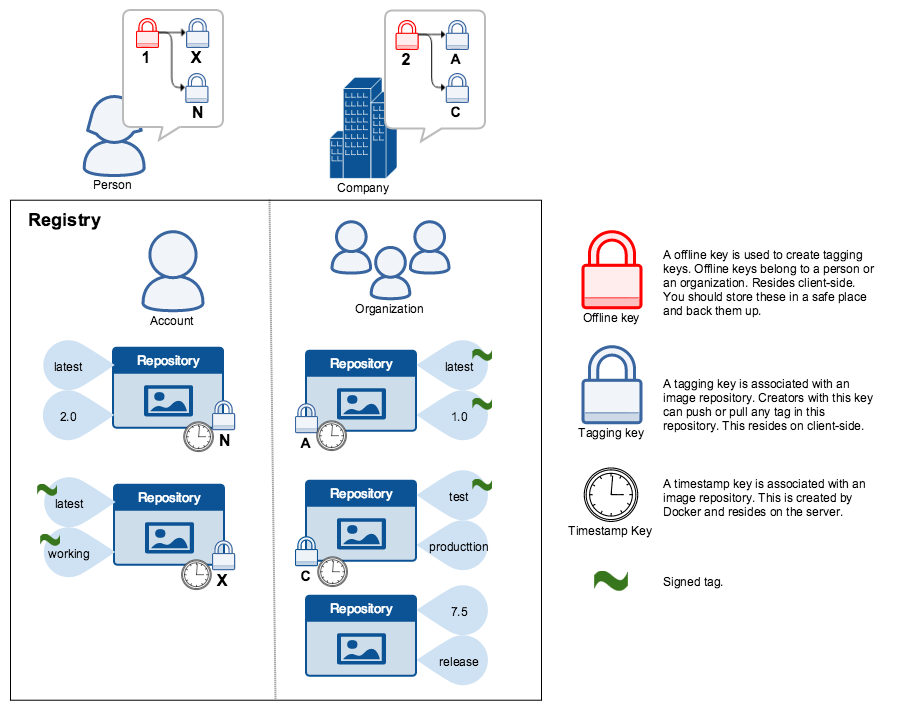
\includegraphics[width=15cm]{figuras/trust_components.png}}
\caption{Relación entre as chaves do Docker Content Trust}
\small
\centerline{Fonte: \url{https://docs.docker.com/engine/security/trust/content_trust/}}
\label{trust_components}
\end{figure}

\section{Singularity}

A validación das imaxes en Singularity é realizada mediante a integración de \textit{hashing} \gls{SHA}-256. Singularity prové un método de validación dos contedores que permite asegurar que a imaxe dun contedor que está a ser distribuído non foi alterada. Despois do proceso de \textit{bootstraping}, o \textit{hash} \gls{SHA}-256 é xerado e amosado ao usuario. Cando a imaxe é corrida máis adiante empregando a opción {\it --hash}, o seu \textit{hash} é rexenerado e amosado ao usuario.\\

O mecanismo non é tan complexo como o existente na tecnoloxía de Docker, pero segundo avisos do equipo de desenvolvemento de Singularity, a versión 3 desta tecnoloxía incluirá diversas melloras no referente a este tema \cite{SingularityLabNotes} (versión actual: 2.5.1). Por exemplo, un mecanismo similar ao de Docker no que só se poderán empregar contedores asinados, ou sistema de montaxe de contedores que permita garantir a orixe dos contedores no que poderiamos escoller só permitir executar contedores creados en certos sitios de confianza. \cite{SingularityRemoteBuild}

\section{Udocker}

Udocker non posúe ningún mecanismo propio de validación, polo que de querer aplicar un proceso de validación empregando Udocker debemos depender do Docker Content Trust explicado na sección \ref{dockerContentTruste}. Neste caso, sería preciso ter a tecnoloxía Docker instalada no sistema.

\cleardoublepage
\chapter{Redes}
\minitoc
\clearpage

Neste capítulo trataranse as implicacións de seguridade que poidan ter as diferentes tecnoloxías de contedorización segundo o seu modelo de rede.

\section{Docker}

\subsection{Introdución ao modelo de rede de Docker}

O modelo de rede de Docker está composto por un subsistema de rede virtual que permite finalmente aos diferentes contedores conectarse á rede que emprega a máquina anfitrioa.\\

Tal e como vén reflectido na documentación oficial de Docker \cite{docker-networking}, non existe unha única forma de despregar este subsistema de rede, senón que coexisten diversos modelos que podemos escoller baixo libre elección: \textit{bridge, host, overlay, macvlan} ou \textit{none}. Cada un deles pensado para ser empregado en diferentes casos de uso.\\

Analizaremos con detemento o modo \textit{bridge}, posto que é o modo por defecto no que o subsistema de rede de Docker é despregado, ademais de ser o modo recomendado para executar contedores independentes que se precisan comunicar. É dicir, cando iniciamos Docker, unha rede \textit{bridge} é creada automaticamente, e será empregada por defecto polos novos contedores \cite{docker-bridge-networks}. Este modo de execución é o máis común, xa que normalmente non interesa executar un contedor illado, senón que se poida comunicar co exterior.\\

Dende un punto de vista arquitectónico, todos os contedores conectados en rede nun anfitrión Docker mediante unha interface \textit{bridge} son equivalentes a máquinas físicas conectadas mediante un \textit{switch Ethernet} común \cite{docker-security}. Unha aproximación visual deste modelo de rede pode ser observada na figura \ref{DockerTopology}\\

\begin{figure}
\centerline{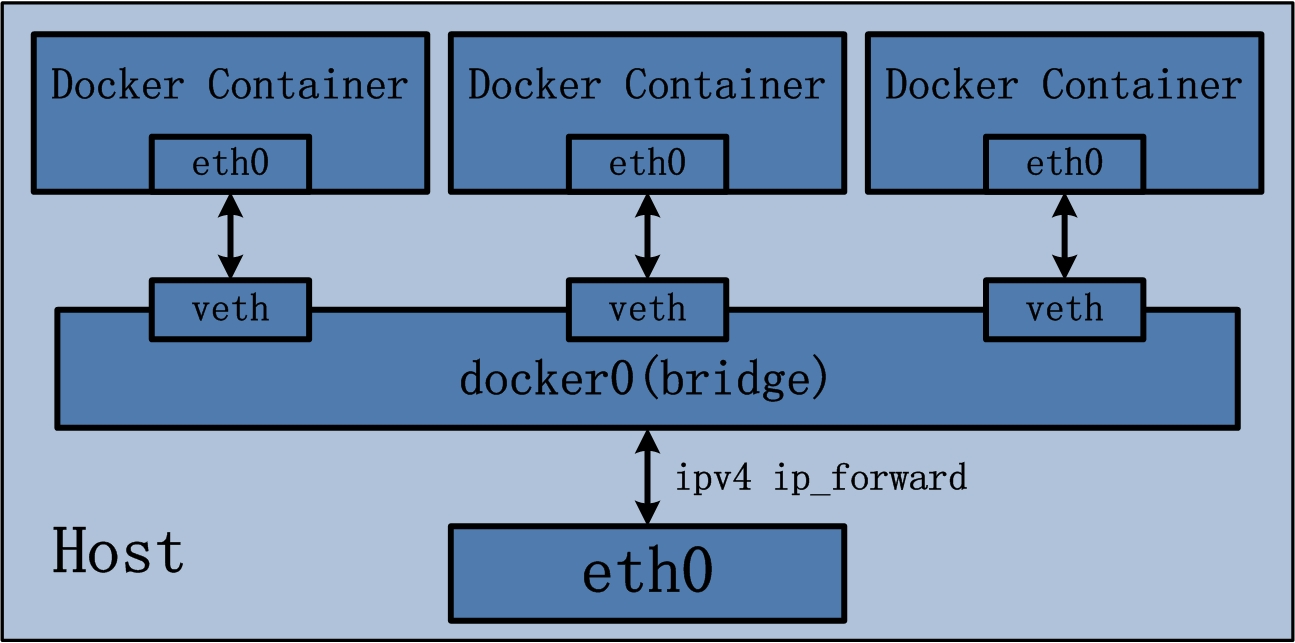
\includegraphics[width=15cm]{figuras/Docker_Topology.jpg}}
\caption{Modelo de rede \textit{bridge} de Docker}
\small
\centerline{Fonte: \url{http://prog3.com/sbdm/blog/shlazww/article/details/47284675}}
\label{DockerTopology}
\end{figure}

Polo tanto, cando se crea un novo contedor Docker, tamén se establece unha nova interface virtual \textit{Ethernet} cun nome único e conéctase ao nomeado \textit{bridge} ou ponte de rede. Esta interface estará conectada ao interface de rede \textit{eth0} do contedor, permitindo así mandar paquetes á ponte dende o mesmo. Este modelo de conectividade establecido por defecto por Docker é susceptíbel a ataques como \gls{ARP} \textit{spoofing} ou \gls{MAC} \textit{flooding}, posto que a ponte permite o reenvío (\textit{forwarding}) de todos os paquetes recibidos sen ningún tipo de filtrado \cite{Securing-Docker-Containers-from-Denial-of-Service}.\\

\subsection{Explotación de vulnerabilidades}

Detectado un posíbel vector de ataque por mor da estrutura de rede seguida por Docker, cómpre realizar probas que aseguren dito comportamento.

Para poder comprobar que as vulnerabilidades previamente detectadas son realmente un posíbel vector de ataque na emprega de contedores Docker, creouse unha pequena estrutura de contedores coa axuda de Docker Compose\footnote{\url{https://docs.docker.com/compose/}}, tal e como ven especificado no anexo \ref{codigo-arp-spoofing}, conectando en rede aos mesmos. A estrutura creada está composta por:

\begin{itemize}
    \item Un contedor servidor correndo Nginx 1.13.10.
    \item Un contedor cliente correndo Ubuntu Xenial 16.04.
    \item Un contedor atacante correndo Kali Linux 2018.1.
\end{itemize}

Devandita estrutura foi levantada sobre unha máquina virtual Ubuntu Xenial 16.04 aloxada no servizo de computación na nube do \gls{CESGA}. A composición final pode ser apreciada na figura \ref{DiagramaRedeDockerCloud}.\\

\begin{figure}
\centerline{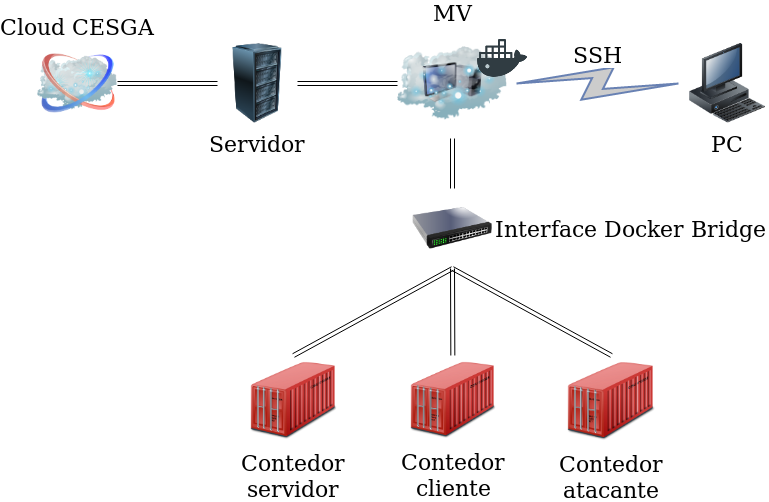
\includegraphics[width=15cm]{figuras/DiagramaRedeDockerCloud.png}}
\caption{Estrutura de contedores Docker para a explotación de vulnerabilidades en rede}
\label{DiagramaRedeDockerCloud}
\end{figure}

Aproveitando as debilidades da rede asociadas ao modelo establecido nos contedores Docker, no que existe un suposto reenderezamento sen ningún tipo de filtrado coa rede da máquina anfitrioa, tratarase de obter tráfico da rede de forma ilexítima dende o contedor atacante namentres se realiza unha comunicación entre os contedores cliente e servidor.

\subsubsection{\gls{ARP} \textit{spoofing}}

%TODO citar to docker or not to docker: El único defecto es que todos los contenedores comparten el mismo puente de red, lo que permite ataques de envenenamiento con el protocolo de resolución de direcciones (ARP) entre contenedores en el mismo host. ---> Namespace isolation and capabilities drop are enabled by default, but cgroups limitations aren’t; they must be enabled on a per-container basis through -a -c options on container launch. The default isolation configuration is relatively strict. The only flaw is that all containers share the same network bridge, enabling Address Resolution Protocol (ARP) poisoning attacks between containers on the same host

\paragraph{Explicación teórica do ataque}~~

Para comprender o que se pretende facer con este ataque, é importante explicar primeiramente de que se trata.\\

O protocolo \gls{ARP}, ou Protocolo de Resolución de Direccións, é un dos protocolos de rede máis básicos pero máis esenciais que existen. É o encargado de resolver o enderezo físico (\gls{MAC}) dunha máquina dado o seu enderezo \gls{IP}. O seu funcionamento baséase no envío dun paquete, \gls{ARP} \textit{request}, a todos os integrantes da rede (\textit{broadcast}), que contén o enderezo \gls{IP} polo que se pregunta e agárdase a que a máquina asociada a devandito enderezo \gls{IP} responda (\gls{ARP} \textit{reply}) co seu enderezo físico correspondente. Cada máquina manterá unha caché cos enderezos traducidos para reducir o retardo, conformando así a denominada táboa \gls{ARP}. Polo tanto, o protocolo \gls{ARP} permite a independencia dos enderezos \gls{IP} e \gls{MAC}.\\

Por mor da falta de mecanismos de autenticación para verificar a identidade do remitente, o protocolo \gls{ARP} ten unha longa historia de propensión como vector de ataques de suplantación \cite{detectingARPSpoofing}. Así, intrinsecamente asociado ao funcionamento deste protocolo, existe o risco de suplantación de \gls{ARP}, ou \gls{ARP} \textit{spoofing}. Este consiste no envío de mensaxes \gls{ARP} falsas á \textit{Ethernet}, conseguindo así asociar o enderezo \gls{MAC} do atacante co enderezo \gls{IP} doutra máquina (a vítima). Como consecuencia deste feito, calquera tráfico dirixido a ese enderezo IP será erroneamente enviado ao atacante, no canto de acadar o seu destino lexítimo.\\

Chegados a este punto, o atacante pode levar a cabo diversas accións:

\begin{itemize}
\item Reenviar os paquetes ao seu verdadeiro destinatario, producíndose un ataque \textit{man-in-the-middle} (MITM), no que ademais pode:
    \begin{itemize}
    \item Reenviar os paquetes sen modificar o seu contido.
    \item Modificar o contido dos paquetes e logo reenvialos ao destinatario.
    \end{itemize}
\item Asociar un enderezo \gls{MAC} inexistente co enderezo \gls{IP} da porta de enlace predeterminada da vítima, evitando así a comunicación da mesma co exterior e producíndose por tanto un ataque de denegación de servizo (\gls{DoS}).
\end{itemize}

Deste xeito, a suplantación \gls{ARP} supón en moitas ocasións o punto de partida para ataques de rede máis sofisticados, como ataques de denegación de servizo, \textit{Man in the middle} ou secuestro de sesións.\\

\paragraph{Realización dun ataque \gls{ARP} \textit{spoofing}}~~

Posto que o risco existe polo simple xeito de conectar unha máquina á rede local mediante \textit{Ethernet}, o modelo de rede de Docker previamente explicado fai que sexa susceptíbel de por si ao ataque. Realizarase unha proba baixo a estrutura da figura \ref{DiagramaRedeDockerCloud} para confirmalo. Os pasos seguidos foron os seguintes:

\begin{enumerate}
\item Previo ao ataque:

En primeira instancia, son comprobados todos os enderezos \gls{IP} e físicos, así como as táboas \gls{ARP} dos contedores cliente e servidor.

\begin{lstlisting}[,caption={Consulta dos enderezos \gls{IP} e físico no contedor atacante}]
root@9f3f255ace4a:/# ifconfig 
eth0: flags=4163<UP,BROADCAST,RUNNING,MULTICAST>  mtu 1500
        inet 172.18.0.4  netmask 255.255.0.0  broadcast 0.0.0.0
        inet6 fe80::42:acff:fe12:4  prefixlen 64  scopeid 0x20<link>
        ether 02:42:ac:12:00:04  txqueuelen 0  (Ethernet)
        RX packets 36822  bytes 82108747 (78.3 MiB)
        RX errors 0  dropped 0  overruns 0  frame 0
        TX packets 36389  bytes 2895807 (2.7 MiB)
        TX errors 0  dropped 0 overruns 0  carrier 0  collisions 0
\end{lstlisting}

\begin{lstlisting}[,caption={Consulta dos enderezos \gls{IP} e físico no contedor cliente}]
root@20136c4451bb:/# ifconfig 
eth0      Link encap:Ethernet  HWaddr 02:42:ac:12:00:02  
          inet addr:172.18.0.2  Bcast:0.0.0.0  Mask:255.255.0.0
          inet6 addr: fe80::42:acff:fe12:2/64 Scope:Link
          UP BROADCAST RUNNING MULTICAST  MTU:1500  Metric:1
          RX packets:5527 errors:0 dropped:0 overruns:0 frame:0
          TX packets:1708 errors:0 dropped:0 overruns:0 carrier:0
          collisions:0 txqueuelen:0 
          RX bytes:30975137 (30.9 MB)  TX bytes:124933 (124.9 KB)
\end{lstlisting}

\begin{lstlisting}[,caption={Consulta dos enderezos \gls{IP} e físico no contedor servidor}]
root@07cecfe068f2:/# ifconfig 
eth0: flags=4163<UP,BROADCAST,RUNNING,MULTICAST>  mtu 1500
        inet 172.18.0.3  netmask 255.255.0.0  broadcast 0.0.0.0
        inet6 fe80::42:acff:fe12:3  prefixlen 64  scopeid 0x20<link>
        ether 02:42:ac:12:00:03  txqueuelen 0  (Ethernet)
        RX packets 3848  bytes 10735169 (10.2 MiB)
        RX errors 0  dropped 0  overruns 0  frame 0
        TX packets 1291  bytes 92650 (90.4 KiB)
        TX errors 0  dropped 0 overruns 0  carrier 0  collisions 0
\end{lstlisting}

Recollidos e estruturados ditos datos obtemos a táboa \ref{direccions-rede}.

\begin{table}[H]
\centering
\caption{Enderezos de rede dos contedores involucrados no ataque}
\label{direccions-rede}
\begin{tabular}{|c|c|c|}
\hline
\textbf{Contedor} & \textbf{Enderezo \gls{IP}} & \textbf{Enderezo físico} \\ \hline
Atacante & 172.18.0.4 & 02:42:ac:12:00:04 \\ \hline
Cliente & 172.18.0.2 & 02:42:ac:12:00:02 \\ \hline
Servidor & 172.18.0.3 & 02:42:ac:12:00:03 \\ \hline
\end{tabular}
\end{table}

\item Execución do ataque:

Para executar o ataque, o contedor atacante enviará en bucle numerosas mensaxes \gls{ARP} aos contedores cliente e servidor, co fin de envelenar as súas respectivas táboas \gls{ARP} e tendo lugar por conseguinte un ataque \textit{man-in-the-middle}. Para isto, empregarase o software \textit{arpspoof}, pertencente ao paquete de utilidades \textit{dsniff}\footnote{\url{https://www.monkey.org/~dugsong/dsniff/}}.

\begin{lstlisting}[,caption={Envelenamento das táboas \gls{ARP} dende o contedor atacante}]
root@9f3f255ace4a:/# arpspoof -i eth0 172.18.0.2 -t 172.18.0.3 &
root@9f3f255ace4a:/# arpspoof -i eth0 172.18.0.3 -t 172.18.0.2 &
\end{lstlisting}

\item Comprobación do ataque:

Unha vez foron enviadas algunhas mensaxes \gls{ARP} co fin de envelenar as táboas dos contedores cliente e servidor, comprobaremos que o ataque se efectuou correctamente. Para iso, inspeccionáronse novamente as táboas \gls{ARP}, onde agora se pode ver con total claridade como as asociacións entre enderezos físicos e \gls{IP} víronse truncados, facendo chegar polo tanto paquetes non lexítimos ao contedor atacante.

\begin{lstlisting}[,caption={Consulta da táboa \gls{ARP} do contedor cliente}]
root@20136c4451bb:/# arp -a
arpspoof_kali_1.arpspoof_default (172.18.0.4) at 02:42:ac:12:00:04 [ether] on eth0
? (172.18.0.1) at 02:42:39:9e:31:24 [ether] on eth0
arpspoof_nginx_1.arpspoof_default (172.18.0.3) at 02:42:ac:12:00:04 [ether] on eth0
\end{lstlisting}

\begin{lstlisting}[,caption={Consulta da táboa \gls{ARP} do contedor servidor}]
root@07cecfe068f2:/# arp -a
arpspoof_kali_1.arpspoof_default (172.18.0.4) at 02:42:ac:12:00:04 [ether] on eth0
? (172.18.0.1) at 02:42:39:9e:31:24 [ether] on eth0
arpspoof_ubuntu_1.arpspoof_default (172.18.0.2) at 02:42:ac:12:00:04 [ether] on eth0
\end{lstlisting}

\paragraph{Realización dun ataque \textit{man-in-the-middle}}~~

Aproveitando o éxito do ataque \gls{ARP} \textit{spoofing}, podemos recibir contidos non asociados ao noso contedor, é dicir, realizarase tamén un ataque \textit{man-in-the-middle}. Para isto, no contedor atacante executaremos a utilidade \textit{urlsnarf}, pertencente tamén ao paquete \textit{dsniff}, o cal mostrará por pantalla todas as URLs solicitadas, como forma de comprobar o éxito deste ataque. No proceso será necesario que, por exemplo, o contedor cliente solicite unha páxina web ao contedor servidor.

\begin{lstlisting}[,caption={Solicitude dunha páxina web dende o contedor cliente ao contedor servidor}]
root@20136c4451bb:/# curl nginx
<!DOCTYPE html>
<html>
.
.
.
</html>
\end{lstlisting}

\begin{lstlisting}[,caption={Escoita de solicitudes web con \textit{urlsnarf} dende o contedor atacante}]
root@9f3f255ace4a:/# urlsnarf -i eth0
urlsnarf: listening on eth0 [tcp port 80 or port 8080 or port 3128]

arpspoof_ubuntu_1.arpspoof_default - - [06/Apr/2018:08:57:08 +0000] "GET http://nginx/ HTTP/1.1" - - "-" "curl/7.47.0"
\end{lstlisting}

Deste xeito, queda demostrado que o envelenamento se efectuou con éxito e que o contedor atacante é quen de escoitar as conexión que se realizan entre os outros contedores, tendo por tanto éxito o ataque \textit{man-in-the-middle}, o cal ten serias consecuencias, como podería ser a modificación do contido dos paquetes intercambiados se así quixer, ou efectuar un ataque de denegación de servizo.

\end{enumerate}

\subsubsection{\gls{MAC} \textit{flooding}}

\paragraph{Explicación teórica do ataque}~~

Continuando coas debilidades asociadas ao protocolo \gls{ARP}, efectuaremos un ataque de \gls{MAC} \textit{flooding}. Este ataque ten como intención comprometer a seguridade dos conmutadores de rede. Normalmente, estes conmutadores manteñen unha táboa \gls{ARP}, como xa foi explicado no ataque de \gls{ARP} \textit{spoofing}, mais neste caso, o obxectivo a acadar é facer caer dita táboa. Para logralo, o atacante envía numerosas peticións \gls{ARP} ao conmutador, até facer desbordar a súa táboa \gls{ARP} interna, provocando que os enderezos físicos e \gls{IP} dos usuarios lexítimos sexan excluídos. Cando se chega a dito punto, o conmutador non posúe información sobre a quen debe enviar os paquetes entrantes, polo que se ve na obriga de entrar en modo \textit{hub}, reenviando todos os paquetes entrantes a todos os dispositivos conectados no mesmo, actuando así nun modo \textit{broadcast}.\\

A principal diferenza entre un ataque de \gls{MAC} \textit{flooding} e un de \gls{ARP} \textit{spoofing} é que o primeiro está dirixido a un obxectivo moito máis xeral, un conmutador da rede, mentres que que o segundo ten como fin a confusión entre enderezos específicos. Ademais, o ataque de \gls{MAC} \textit{flooding} posúe a vantaxosa e perigosa característica de que ao non estar enfocado nun obxectivo xeral, e apoiándose no funcionamento do protocolo \gls{ARP}, pode chegar a propagarse pola totalidade da rede, coa provocación de desbordamentos de táboas \gls{ARP} encadeados entre os diferentes dispositivos que compón dita rede.

\paragraph{Realización dun ataque \gls{MAC} \textit{flooding}}~~

Aproveitando novamente a estrutura da figura \ref{DiagramaRedeDockerCloud}, realizarase un ataque de \gls{MAC} \textit{flooding}. Se o ataque ten éxito, deberiamos ser quen de ollar paquetes alleos dende o contedor atacante, pertencentes aos outros contedores da rede. A súa execución segue os seguintes pasos:

\begin{enumerate}
\item Previo ao ataque:

Escoita de todos os paquetes que cheguen á rede do contedor atacante:
    
\begin{lstlisting}[,caption={Escoita dos paquetes entrantes á rede do contedor atacante}]
root@9403362d194e:/# tcpdump -i eth0 -X -vv
tcpdump: listening on eth0, link-type EN10MB (Ethernet), capture size 262144 bytes
\end{lstlisting}

\item Execución do ataque:

Enviamos numerosas solicitudes \gls{ARP} dende o contedor atacante á rede. Para automatizar o proceso, facemos uso da ferramenta \textit{macof}, pertencente ao paquete de utilidades \textit{dsniff}\footnote{\url{https://www.monkey.org/~dugsong/dsniff/}}.

\begin{lstlisting}[,caption={Execución do ataque \textit{macof}}]
root@9403362d194e:/# macof 
23:35:f0:47:32:2a 1:a9:ca:38:a8:dd 0.0.0.0.33552 > 0.0.0.0.17981: S 215025915:215025915(0) win 512
b1:7b:e5:0:e7:e4 91:fe:39:2e:2e:ae 0.0.0.0.12840 > 0.0.0.0.19430: S 1017556768:1017556768(0) win 512
98:8:33:39:31:80 a5:58:b9:5f:dd:4d 0.0.0.0.20270 > 0.0.0.0.5234: S 795884266:795884266(0) win 512
a8:8:54:1e:6d:e7 7c:2b:df:20:c8:8 0.0.0.0.8086 > 0.0.0.0.51239: S 1625463231:1625463231(0) win 512
25:e9:f:7d:38:77 1f:89:2b:11:0:13 0.0.0.0.43039 > 0.0.0.0.55182: S 199622377:199622377(0) win 512
e8:85:91:32:9a:4c ba:52:5e:41:d7:f0 0.0.0.0.56124 > 0.0.0.0.27045: S 1368523758:1368523758(0) win 512
c0:80:e:b:7c:7c 2d:23:d8:9:2a:d8 0.0.0.0.35983 > 0.0.0.0.9435: S 1477501491:1477501491(0) win 512
.
.
\end{lstlisting}

\item Comprobación do ataque:

Pasado un tempo, no que as numerosas solicitudes \gls{ARP} xa fixeron desbordar a táboa \gls{ARP} do conmutador (a interface Docker \textit{Bridge}), consúltase o estado dos paquetes recibidos polo contedor atacante. Nun principio a idea era que se puidesen ollar paquetes pertencentes á subrede Docker despregada, non obstante os resultados trocaron ben distintos. Comezaron chegar paquetes pertencentes ao exterior da subrede creada para a proba, evidenciando o alcance do ataque e tamén unha posíbel mala xestión da seguridade da rede da \gls{MV} sobre a que se construíu a estrutura para a realización desta proba. A imaxe \ref{ataqueMacFlooding} amosa este feito (os enderezos \gls{IP} foron ocultados para respectar a privacidade). Deste xeito, dende o contedor atacante é posíbel observar conexións doutras máquinas con páxinas externas como, por exemplo, a Universidade de Texas.

\begin{figure}[H]
\centerline{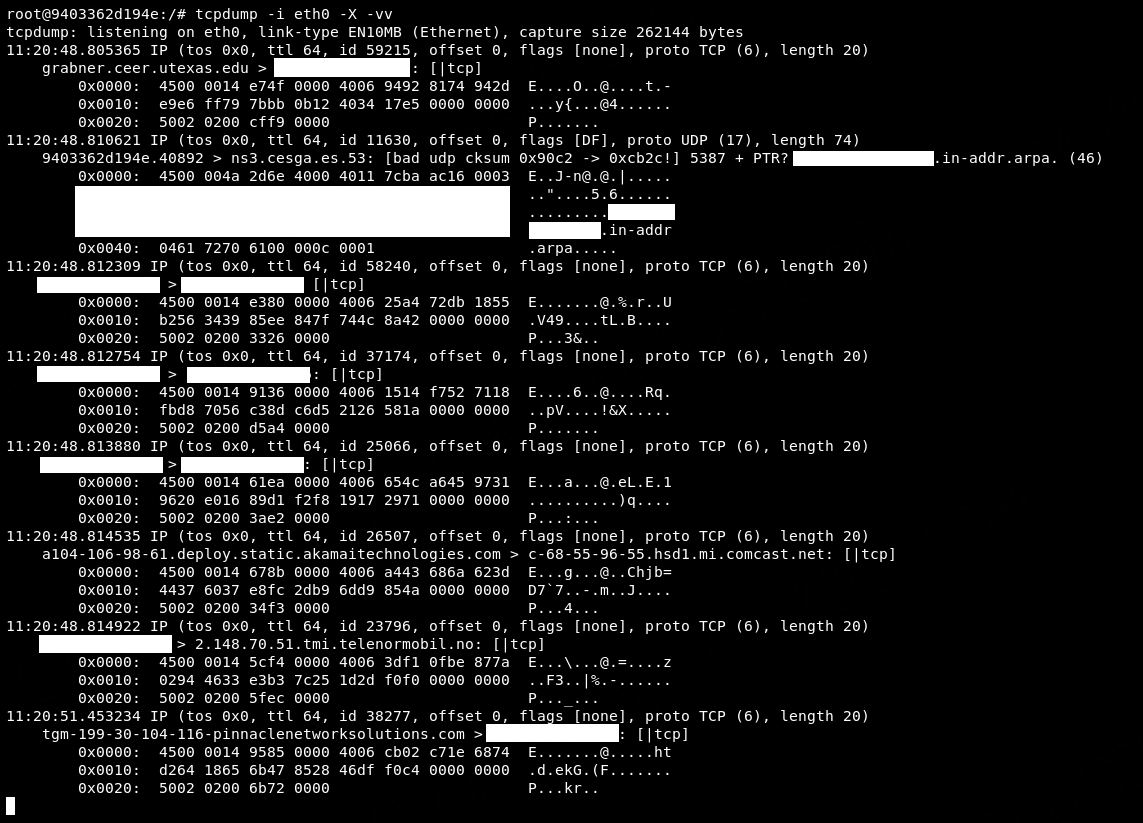
\includegraphics[width=15cm]{figuras/ataqueMacFlooding.png}}
\caption{Paquetes lidos dende o contedor atacante no transcurso do ataque \gls{MAC} \textit{flooding}}
\label{ataqueMacFlooding}
\end{figure}

\end{enumerate}

\section{Singularity}

\subsection{Introdución ao modelo de rede de Singularity}

Singularity emprega a mesma rede que calquera outro proceso da máquina anfitrioa. Posto que Singularity non emula ningún paradigma de virtualización a nivel de hardware, non é necesario separar as redes do espazo illado dos contedores do resto do sistema, xa que, en principio, non existe o concepto de escalada de privilexios dentro dos contedores Singularity. É dicir, os programas executados baixo un contedor Singularity terán os mesmos privilexios que se o fixese dende fóra, polo que os riscos asociados á emprega da rede non dependerán da emprega deste tipo de contedores. \cite{SingularityHPC}

\subsection{Inviabilidade do ataque}

Grazas a este modelo de rede, Singularity non pode ser vulnerábel aos ataques aos que Docker, por defecto, si que o é, posto que comparte a rede coa da propia máquina anfitrioa e os permisos dentro do contedor son os mesmos que fóra del.\\

Un posíbel vector de ataque viría dado pola escalada de privilexios e tentar executar programas de rede con permisos de superusuario dentro do contedor. Este feito será estudado con máis detalle na sección \ref{demo-fail-escalada}.

\section{Udocker}

\subsection{Introdución ao modelo de rede de Udocker}

Tal e como foi indicado na presentación desta tecnoloxía na sección \ref{introUdocker}, Udocker nunca acada privilexios avanzados de superusuario, polo que ten certas limitacións sobre a rede. Ademais, Udocker non desprega ningún tipo de entorno de rede adicional, simplemente emprega a rede da máquina anfitrioa. Isto é trivial no sentido de que para poder despregar cambios na rede son precisos permisos de superusuario, requirindo UID=0, e polo tanto, Udocker non pode facer nada.

\subsection{Inviabilidade do ataque}

Polos motivos expostos, ao igual que a tecnoloxía de Singularity, con Udocker tampouco é posíbel efectuar os mesmos tipos de ataque sobre a rede que si son viábeis en Docker. Para que estes ataques puidesen ser efectuados, Udocker debería ter un control máis avanzado sobre as redes, só alcanzábel coa outorga de privilexios de superusuario, que nunca ten.

\cleardoublepage
\chapter{Limitación de recursos}
\minitoc
\clearpage

\section{Introdución}

A limitación dos recursos físicos é unha cuestión crítica no referente á seguridade do sistema, xa que un contedor malicioso podería facer uso exhaustivo dos mesmos, chegando a ocupar a práctica totalidade destes e prexudicando así a outros contedores aloxados na mesma máquina, ou mesmamente á propia máquina anfitrioa, podéndose producir así un ataque de denegación de servizo (\gls{DoS}) \cite{OS-level-security}. Numerosos aspectos deben ser tidos en conta para asegurar a seguridade integral do sistema no referente á utilización adecuada dos recursos físicos. Dividiremos o estudo en: CPU, memoria, disco e rede.\\

Analizaremos as diferentes respostas a este tipo de sobreempregas de recursos, tentando facer unha comparativa entre execucións debidamente controladas e outras que non o estarán, para o cal empregaranse pequenas aplicacións contedorizadas.

\section{Modelo de limitación de recursos de Docker}

Docker relega algunha das súas funcionalidades de seguridade directamente nas características inherentes do \textit{kernel} de GNU/Linux. Polo tanto, o límite dos privilexios entre os contedores e a máquina anfitrioa xa foi deseñado. Os controis técnicos que levan este límite inclúen o illamento de procesos mediante os espazos de nomes (\textit{namespaces}\footnote{http://man7.org/linux/man-pages/man7/namespaces.7.html}), permitindo así illar usuarios, procesos, redes ou dispositivos, e administración dos recursos mediante \textit{cgroups}\footnote{http://man7.org/linux/man-pages/man7/cgroups.7.html}. Ambos, espazos de nomes e \textit{cgroups}, fusionáronse a partir da versión 2.6.24 do \textit{kernel} de GNU/Linux. Deste xeito, os contedores Docker execútanse baixo un suposto entorno illado e controlado na máquina anfitrioa. No referente aos límites de recursos, tema principal desta sección, debemos pór a nosa atención nos \textit{cgroups}, posto que o seu obxectivo é precisamente que un proceso non tome todos os recursos dispoñíbeis do sistema. Isto inclúe os recursos partillados de CPU, memoria, ancho de banda da rede e E/S de disco \cite{To-Docker-Or-Not-To-Docker}. \\

Debido a estas delegacións de seguridade sobre os \textit{cgroups}, non debemos influír na súa funcionalidade (e polo tanto no control de seguridade que realiza) con opcións de Docker como pode ser o \textit{flag --privileged}, que eleva as capacidades do contedor e elimina tamén as limitacións impostas polos \textit{cgroups} \cite{state-of-art-docker-security}, deixando ao sistema vulnerábel. É dicir, Docker posúe opcións avanzadas que permiten outorgar dun maior número de privilexios aos seus contedores, evadindo os controis realizados polos \textit{cgroups}, por exemplo; mais estas opcións poden supor un gran risco para o noso sistema e debémolas evitar sempre que nos sexa posíbel.\\

A mellora de seguridade aportada pola axuda dos \textit{cgroups} e do espazo de nomes non deixa de mellorar cada día, polo que resulta importante manter as tecnoloxías de contedorización actualizadas para obter as últimas correccións de seguridade. Por exemplo, até a versión 1.10 de Docker, non existía un espazo de nomes para o usuario, o que pode ser considerado un risco crítico. Se un proceso conseguise dalgunha forma ``rachar'' o contedor e saír del, executándose na máquina anfitrioa, ao non existir un espazo de nomes para os usuarios, o proceso obtería os mesmos privilexios que tiña dentro do contedor, mais na máquina anfitrioa. Polo tanto, se o proceso tiña privilexios de superusuario (\gls{UID}=0) no interior do contedor, tamén gañaría privilexios de superusuario no exterior, podendo modificar o sistema a pracer. Produciríase entón un ataque de escalada de privilexios, no que un usuario non autorizado obtería privilexios sobre o sistema aos que non debería ter acceso. Aínda que as posibilidades de que isto suceda son moi poucas, non debe ser considerado coma algo insignificante.\\

Como xa foi comentado, a partir da versión 1.10 de Docker os espazos de nomes dos usuarios foron tidos en conta, supondo unha das actualizacións de seguridade máis importantes desta tecnoloxía de contedorización. Dende dita versión, cada proceso posúe o seu propio conxunto de identificadores para usuarios e grupos. Por exemplo, se un proceso dentro do contedor posúe o \gls{UID} 0, pertencente ao superusuario, na máquina anfitrioa podería estar mapado a un \gls{UID} calquera, como por exemplo o 3000, pertencente a un usuario non privilexiado. Este mapado evita que procesos executados dentro dun contedor poidan obter permisos de superusuario fóra do contedor. \cite{state-of-art-docker-security} \\

Non obstante, debemos configurar o noso sistema con moita cautela, posto que aínda que dende a versión 1.10 estes espazos de nomes foros introducidos en Docker, dita característica está dispoñíbel, mais non está activada por defecto \cite{docker-security}. É labor do administrador do sistema asegurar a súa correcta configuración e seguridade. Para isto, pode facer emprega de ferramentas de auditoría como a descrita na sección \ref{DockerBeckAuditTool}.

\section{Modelo de limitación de recursos de Singularity}
\label{modeloLimitacionRecursosSingularity}

A diferenza de Docker, o modelo de funcionamento dos contedores Singularity entende que a limitación de recursos queda fóra da súa xurisdición, posto que os contedores Singularity foron deseñados para correr como calquera outra aplicación do sistema. É dicir, os procesos poden ser observados dende fóra do contedor e, polo tanto, xestionados por ferramentas externas como calquera outro proceso do sistema. Polo tanto, enténdese que estas limitacións deben ser xestionadas por un administrador de recursos propio do sistema \cite{singularity-limits}; idea que cobra máis sentido se temos en conta que son un tipo de contedores creados especialmente para o seu uso en \gls{HPC}.\\

Tendo en conta o marco de traballo no que este proxecto se desenvolve, no cal se estuda a seguridade en entornos \gls{HPC}/\textit{Cloud} nas infraestruturas do \gls{CESGA}, poden ser aproveitadas funcionalidades xa implantadas no sistema para a repartición e limitación dos recursos. Deste xeito, o xestor da carga de traballo para \gls{HPC} empregado nestes momentos no centro é Slurm, tal e como foi explicado na sección \ref{infraestruturaSlurm}. Así, a meirande parte das tarefas de distribución da carga de traballo, e polo tanto de asegurar a limitación dos recursos físicos, dependen deste xestor.

\section{CPU e memoria}

Estes dous recursos físicos foron xuntados nunha soa sección posto que a súa forma de control e limitación faise dun xeito practicamente idéntico, presentando soamente diferenzas dependendo da tecnoloxía de contedorización a empregar.

\subsection{Docker}

Grazas á delegación nos \textit{cgroups}, Docker posúe a funcionalidade de poder limitar a cantidade de memoria que cada contedor pode empregar, evitando así que un contedor ocupe toda a memoria e deixe sen recursos a outros contedores, ou peor aínda, á propia máquina anfitrioa \cite{state-of-art-docker-security}. Do mesmo xeito, a CPU tamén é controlada polos \textit{cgroups}, baixo a mesma premisa.

\subsubsection{Probas de limitación de CPU e memoria con Docker}

Para a realización das probas de memoria, escribiuse un sinxelo código en C, dispoñíbel no anexo \ref{consumidorMemoria}, cuxa lóxica baséase nun bucle infinito de reservas dinámicas de memoria, sen facer liberación da mesma. Tras pór a proba dito código, observouse que o contedor era parado automaticamente polo sistema. Isto resultou ser porque, por defecto, Docker conta cunha ferramenta de prevención de \textit{out-of-memory} (\gls{OOM}). É dicir, se os límites son superados, o sistema encargarase de matar pola súa conta aos procesos. De non querer que isto suceda, deberiamos activar o \textit{flag} \textit{--oom-kill-disable} cando lanzamos un contedor Docker. Obviamente, esta medida resultaría contraproducente contra a defensa de un ataque de \gls{DoS}, polo que debemos evitar empregala sempre que poidamos.\\

Neste caso, para poder facer uso do pequeno código de proba, desactivaremos esta opción. Para a realización da proba, crearemos un contedor Docker con límites de memoria e CPU, que serán xestionados polos \textit{cgroups}. Cando lanzamos o programa xa compilado, coa opción de de \gls{OOM} desactivada, podemos ver como a memoria e a utilización da CPU axústanse aos límites outorgados no momento de invocación do contedor. A forma de invocar ao contedor só permite a emprega de 1.5 de CPU e de 500 MB de memoria.

\begin{lstlisting}[,caption={Emprega de límites de CPU e memoria en contedores Docker}]
docker run --memory=500m --cpus="1.5" --oom-kill-disable -it ubuntu /bin/bash
\end{lstlisting}

Para a comprobación dos cumprimento dos límites establecidos empregouse a ferramenta \textit{Docker Stats}\footnote{\url{https://docs.docker.com/engine/reference/commandline/stats/}}, tal e como pode ser observado na figura \ref{MemoriaFull}. Tamén se comprobou que a emprega de CPU por parte da máquina anfitrioa non superaba os límites, tal e como amosa a figura \ref{CPUDocker}.

\begin{figure}[]
\centerline{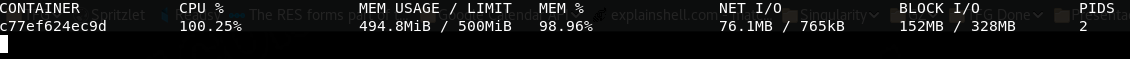
\includegraphics[width=15cm]{figuras/MemoriaFull.png}}
\caption{Emprega total de CPU e memoria dun contedor Docker con límites}
\label{MemoriaFull}
\end{figure}

\begin{figure}[]
\centerline{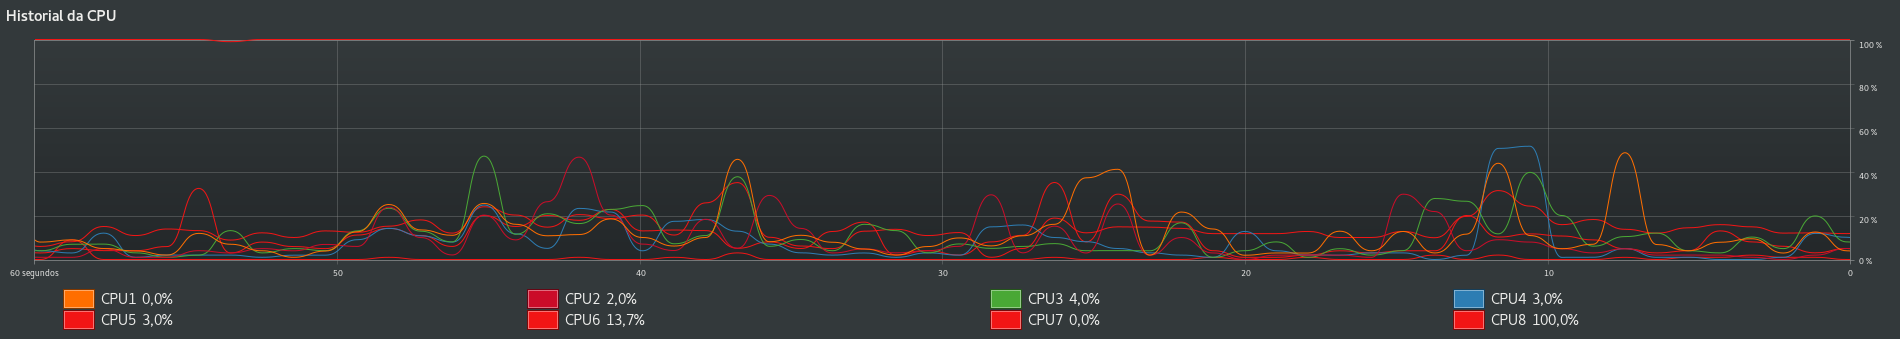
\includegraphics[width=15cm]{figuras/CPUDocker.png}}
\caption{Revisión da CPU empregada na máquina anfitrioa}
\label{CPUDocker}
\end{figure}

\subsection{Singularity}

Tal e como foi explicado na sección \ref{modeloLimitacionRecursosSingularity}, Singularity entende que non é a súa xurisdición o control dos recursos do sistema, ao estar deseñado para correr como unha aplicación máis do sistema. Deste xeito, neste caso, CPU e memoria son dous dos factores claramente controlados polo xestor de recursos Slurm. Así, á hora de lanzar un proceso con este xestor, empregando comandos como {\it srun} ou {\it sbatch}, podemos indicar \textit{flags} que indiquen con exactitude os recursos dos que queremos facer uso. Abstraéndonos do proceso, Slurm encargarase de que o usuario non poida superar os límites que solicitou. Por exemplo, algunhas das opcións máis amplamente empregadas e que dan solución ao problema dos límites de recursos son:

\begin{itemize}
    \item \textbf{\textit{-N} ou \textit{--nodes}:} solicita o mínimo número de nodos que deben ser reservados para certo traballo. Tamén é posíbel indicar o máximo número de nodos. No caso de indicar soamente un número, ese indicará o mínimo e o máximo. No caso de non haber nodos suficientes para o traballo indicado nese momento, o traballo acadará un estado de ``pendente'', á espera de que os nodos precisos sexan liberados.
    \item \textbf{\textit{-n} ou \textit{--ntasks}:} indica o número máximo de tarefas a desenvolver e fornece os recursos suficientes. O valor predeterminado é dunha tarefa por cada nodo.
    \item \textbf{\textit{--ntasks-per-core}:} pensado para ser executado en combinación coa opción {\it --ntasks}, indica o número máximo de tarefas a ser executadas por cada núcleo.
    \item \textbf{\textit{--ntasks-per-node}:} indica o número de tarefas a ser desenvolvidas por cada nodo. De ser empregado xunto coa opción {\it --ntasks}, devandita opción terá prioridade no canto desta.
    \item \textbf{\textit{--mem}:} indica a memoria \gls{RAM} que poderá obter cada nodo. Se facemos especificación dun tamaño de memoria igual a cero, tratarase como un caso especial e outorgarase a ese traballo toda a memoria dispoñíbel de cada nodo. Ter en conta que se traballamos cun \textit{cluster} heteroxéneo, o límite de memoria virá dado polo nodo cun tamaño de memoria máis pequeno.
    \item \textbf{\textit{--mem-per-cpu}:} indica a memoria \gls{RAM} que será preciso asignar por cada CPU. Destacar que as opcións {\it --mem-per-cpu} e {\it --mem} son mutuamente exclusivas.
\end{itemize}

\section{Disco}

Cando falamos das limitacións a ter en conta no referente á emprega de disco, debemos discernir dous casos diferenciados. O primeiro deles fai referencia á E/S, posto que un contedor que faga amplo uso deste factor podería ter un impacto prexudicial noutros contedores ou na mesma máquina anfitrioa. O segundo caso fai referencia á emprega de disco no que ten que ver coa súa capacidade.\\

Por exemplo, cando se empregan algúns dos controladores de almacenamento como pode ser \textit{aufs}, Docker non limita a emprega de disco dos contedores. Un contedor cun volume de almacenamento pode encher este volume e afectar a outros contedores na mesma máquina anfitrioa, ou incluso á mesma, se o almacenamento especificado na ruta ``{\it /var/lib/docker}'' non está montado nunha partición separada \cite{To-Docker-Or-Not-To-Docker}.

\subsection{Cotas de disco}
\label{quotas}

Para evitar que un contedor empregue a totalidade ou meirande parte do disco, impedindo a correcta execución doutros, cómpre aplicar políticas de limitación no uso do mesmo. Estas políticas poden ser aplicadas doadamente coa emprega de cotas, permitindo establecer diversidade de límites en función dos usuarios do sistema.\\

Grazas a este feito, os contedores Singularity quedarán perfectamente limitados no referente á utilización do disco. Pola súa contra, os contedores Docker, posto que son controlados polo demo Docker con permisos de superusuario, non se verán limitados, xa que o superusuario terá a capacidade {\it CAP\_SYS\_RESOURCE}\footnote{\url{http://man7.org/linux/man-pages/man7/capabilities.7.html}} activada, a cal permite ignorar os límites de cotas de disco, entre outras cousas.\\

Para comprobar este feito, realizouse unha proba de concepto dentro dunha máquina virtual Ubuntu Xenial 16.04, na que se estableceron cotas de disco para un determinado usuario e posteriormente tentouse escribir un ficheiro que superase as limitacións establecidas, facendo uso de contedores baseados en Alpine Linux 3.7.0 (que presentan a característica de que o seu sistema base está deseñado para ocupar só 4-5MB , excluíndo o \textit{kernel}). As limitacións escollidas foron de 10MB \textit{soft} e de 100MB \textit{hard}. O proceso de aplicación destas cotas pode ser consultado no apéndice \ref{scriptQuotas}.

\subsubsection{Probas de cotas nun contedor Docker}

\begin{lstlisting}[,caption={Escritura en disco excedendo cuota máxima en contedor Docker}]
nuevousuariocuotas@localhost:~$ docker run -ti alpine
/home # dd if=/dev/zero of=fichero bs=200M count=1
1+0 records in
1+0 records out

#Saimos do contedor
nuevousuariocuotas@localhost:~$ docker ps -s 
CONTAINER ID        IMAGE               COMMAND             CREATED             STATUS              PORTS               NAMES               SIZE
1aba32e99ce5        alpine              "/bin/sh"           4 minutes ago       Up 3 seconds                            gifted_bohr         210MB (virtual 214MB)
\end{lstlisting}

No caso do contedor executado baixo a tecnoloxía de Docker, a escritura é posíbel e os límites son superados. Se ao rematar comprobamos o tamaño actual do contedor, pódese ver coma ocupa un total de 210MB, superando así a cota total de disco establecida para o usuario.\\

\subsubsection{Probas de cotas nun contedor Singularity}

\begin{lstlisting}[,caption={Escritura en disco excedendo cuota máxima en contedor Singularity}]
dd if=/dev/zero of=fichero bs=200M count=1
dd: error writing 'fichero': Disk quota exceeded
1+0 records in
0+0 records out
102354944 bytes (102 MB, 98 MiB) copied, 0.701354 s, 146 MB/s
\end{lstlisting}

Como se pode ver, as cotas entran en xogo no caso dos contedores Singularity, impedindo a escritura de ficheiros unha vez o límite máximo é excedido.\\

\subsubsection{Alternativa a aplicar en Docker}

A execución de cotas sobre contedores Docker non resulta efectiva. De todos xeitos, esta tecnoloxía presenta unha xestión sobre os discos máis avanzada, que debe ser estudada con maior detemento.\\

Docker amósanos a posibilidade de almacenar datos no disco dende dúas perspectivas ben diferenciadas:

\begin{enumerate}
    \item \textbf{Almacenamento persistente no disco:} os datos non se perden unha vez remata a execución do contedor.
    \item \textbf{Almacenamento volátil:} os datos soamente son accesíbeis namentres o contedor está executándose.
\end{enumerate}

Para facer esta diferenciación de tipos de almacenamento, Docker presenta varios tipos de montaxe do disco, tal e como pode ser observado na figura \ref{typesOfMountsDocker}. Unha vez dentro do contedor, os datos veranse da mesma forma, no entanto é importante diferencialos para facer un uso adecuado do disco. Así, distinguimos:

\begin{figure}
\centerline{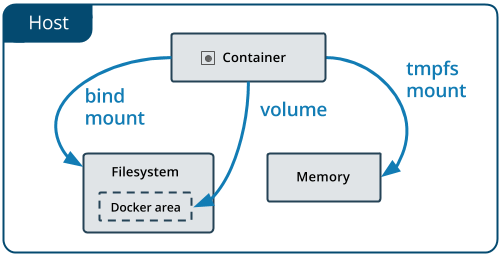
\includegraphics[width=15cm]{figuras/typesOfMountsDocker.png}}
\caption{Tipos de montaxe de disco en Docker}
\small
\centerline{Fonte: \url{https://docs.docker.com/storage/}}
\label{typesOfMountsDocker}
\end{figure}

\begin{enumerate}
    \item \textbf{Volumes}: almacenados nalgunha parte do sistema de ficheiros que será xestionado por Docker. Os procesos non pertencentes a Docker non deberían modificar o seu contido, e é considerada a mellor forma de realizar un almacenamento persistente empregando contedores Docker, xa que posúen a característica de estar illados da propia máquina anfitrioa. Ademais, un mesmo volume pode ser compartido entre varios contedores e son doadamente transportábeis cara outra máquina. O seu tamaño pode ser xestionado mediante comandos propios de Docker, pondo solución así a posíbeis ataques de denegación de servizo.
    \item \textbf{\textit{Bind mounts}}: son a outra forma de almacenamento persistente xestionada por Docker. O seu funcionamento baséase na emprega dun espazo de disco compartido coa propia máquina anfitrioa (polo que procesos externos poderían modificar estes datos). Un efecto secundario deste feito é que é posíbel facer cambios no sistema de ficheiros da máquina anfitrioa con permisos de superusuario, pudendo chegar a modificar ou eliminar datos importantes do sistema. Polo tanto, esta forma de almacenamento ten importantes implicacións de seguridade, incluíndo un posíbel impacto nos procesos do sistema non referentes a Docker.
    \item \textbf{Montaxes \textit{tmpfs}}: supoñen a forma de almacenamento non persistente, gardando os datos soamente de forma temporal no tempo de vida do contedor e non chegando a escribir no sistema de ficheiros da máquina anfitrioa. A emprega deste tipo de montaxes pode ser moi interesante se estamos a facer uso de contedores para despregamentos rápidos e lixeiros, coma podería ser un contedor para probas.
    
    Este tipo de almacenamento presenta a perigosa característica, dende o punto de vista da seguridade informática, de que por defecto non posúe ningún tipo de limitación no espazo de disco que certo contedor poida empregar. En troques, si que é posíbel establecer controis e restrinxir o espazo máximo a empregar dentro de cada contedor, coa limitación de que soamente é factíbel baixo a emprega de certos controladores. Docker admite varios controladores de almacenamento, empregando unha arquitectura conectábel, sendo estes os encargados de como as imaxes e os contedores son almacenados e xestionados polo \textit{host}.
    
    Así, se queremos limitar o espazo, deberemos empregar controladores concretos como pode ser \textit{devicemapper}, un framework baseado no \textit{kernel} de GNU/Linux que sustenta moitas das tecnoloxías avanzadas de xestión de volumes neste tipo de sistemas. Debe ser tido en conta que é precisa unha configuración específica para poder empregar este controlador con Docker que non é admitida por todos os sistemas operativos, polo que o seu uso non resulta trivial. Como dato de interese, destacar que \textit{devicemapper} opera a nivel de bloque, no canto de nivel de arquivo, acadando así un rendemento mellor que coa emprega dun sistema de ficheiros a nivel de sistema operativo.
    
    Para comprender un pouco mellor a complexidade asociada, é preciso entender que a elección dun controlador de disco vén limitado por unha serie de dependencias coma poden ser a edición de Docker, o sistema operativo e mesmamente a distribución do mesmo. Tamén poden ser requiridos paquetes a maiores para a súa instalación. Ademais, algúns controladores precisan dun formato específico do sistema de ficheiros da máquina anfitrioa, polo que de existir requirimentos externos que limiten a elección dun sistema de ficheiros específico, isto podería limitar enormemente as nosas opcións. Deste xeito, amósase unha táboa de configuracións consideradas estábeis nas versións máis recentes dalgúns dos sistemas operativos GNU/Linux máis soados:

% \usepackage{graphicx}
\begin{table}[H]
\centering
\caption{Configuracións de controladores de almacenamento}
\label{conf-controladores-almacenamento}
\resizebox{\textwidth}{!}{%
\begin{tabular}{|c|c|}
\hline
\textbf{Distribución GNU/Linux} & \textbf{Controladores de almacenamento recomendados}\\ \hline
Ubuntu & \textit{aufs}, \textit{devicemapper}, \textit{overlay2}, \textit{overlay}, \textit{zfs}, \textit{vfs}\\ \hline
Debian & \textit{aufs}, \textit{devicemapper}, \textit{overlay2}, \textit{overlay}, \textit{vfs}\\ \hline
CentOS & \textit{devicemapper}, \textit{vfs}\\ \hline
Fedora & \textit{devicemapper}, \textit{overlay2} (experimental), \textit{overlay} (experimental), \textit{vfs}\\ \hline
\end{tabular}%
}
\end{table}
    
    Debemos ter en conta que cada controlador terá algunha vantaxe característica sobre os outros, dependendo da configuración propia de cada sistema. Aínda así, estes aspectos quedan fóra do ámbito do estudo da seguridade, polo que non serán estudados con detemento.
    
    Finalmente, é de vital importancia destacar que se é preciso realizar un cambio nos controladores, os contedores que empregasen o controlador anterior, deixarán de ser accesíbeis, sendo preciso realizar unha parada nos mesmos, exportalos a un medio externo e volver a montalos baixo os novos controladores, o que podería supor unha gran desaceleración do sistema. Polo tanto, é relevante realizar unha adecuada elección do controlador.
    
\end{enumerate}

\section{Rede}
\label{QoSRede}

A limitación da rede supón un caso bastante especial, posto que ningunha das tecnoloxías de contedorización a estudar fai un control especial sobre esta, o que podería levar a posíbeis ataques de denegación de servizo. É por iso que cómpre aplicar políticas externas de calidade de servizo que aseguren un funcionamento correcto da mesma.

\subsection{Enfoque de Docker sobre a rede}

As redes que Docker configura até arestora están pensadas para funcionar baixo unha filosofía do ``mellor esforzo'' para todo o tráfico existente. Isto implica que parámetros tales como o ancho de banda, a fiabilidade ou o número de paquetes por segundo non poden ser garantidos. Consecuencia deste feito, a emprega dunha única aplicación que faga un uso intensivo do ancho de banda da rede podería implicar un pobre ou incluso inaceptábel rendemento para calquera outra aplicación que comparta esa rede.\\

Así, a solución pasa pola emprega da denominada calidade de servizo (\textit{Quality of Service}, \gls{QoS}), unha serie de mecanismos que fornecen un trato preferenciado a diferentes tráficos e aplicacións \cite{dockerQoS}. Noutras verbas, non é Docker o encargado de xestionar os límites de recursos das redes, senón que de quixer, debemos ser nós quen, a través de medios alternativos debemos establecelos.

\subsection{Enfoque de Singularity sobre a rede}

Repetindo a idea, Singularity fai uso directo de moitos dos recursos do sistema, incluída a rede, sendo compartida directamente coa máquina anfitrioa. Non existen mecanismos propios de limitación da rede, senón que debe ser administrada por servizos externos.

\subsection{Solución común: \gls{QoS}}

A \gls{QoS} pode ser entendida coma o rendemento da rede tal e como o percibe o usuario final. Os parámetros de \gls{QoS} abranguen todos os aspectos dunha conexión, sendo particularmente importantes:

\begin{itemize}
\item Tasa de transmisión (ancho de banda)
\item Retardo (latencia)
\item Variación do retardo (\textit{jitter})
\item Perda de paquetes
\end{itemize}

Dentro dos sistemas GNU/Linux, a QoS está presente como parte do subsistema de rede \textit{iproute}\footnote{\url{http://linux-ip.net/articles/Traffic-Control-HOWTO/}}, permitindo repartir o ancho de banda en función de distintos criterios e baseando o control nun sistema de colas. A gran flexibilidade que outorga este sistema será útil para poder facer un control diferenciado da rede segundo as tecnoloxías de contedorización empregadas, posto que como quedou patente, non todas empregan o mesmo modelado.\\

Como caso de estudo, farase uso do comando {\it tc}, pertencente ao subsistema \textit{iproute}.

\subsubsection{Probas de limitación de rede con Docker}

O modelo de rede de Docker, no seu funcionamento por defecto, é dicir en modo \textit{bridge}, crea unha interface de rede que é empregada para realizar a conexión entre os contedores e a propia máquina. Aproveitaremos o feito de que Docker permite a creación de diferentes interfaces de rede para a conexión dun ou múltiples contedores para aplicar regras de limitación do tráfico de rede.\\

Realizarase unha proba de concepto na que se limitará a velocidade do tráfico da rede. Aplicarase unha limitación mediante unha disciplina de colas sen facer uso de clases, seguindo unha lóxica bastante simple. Enténdese que se é posíbel aplicar estas limitacións, tamén será posíbel aplicar limitacións máis complexas, que variarán segundo a necesidade do entorno. Así, aplicarase unha disciplina ``TBF'' (\textit{Token Bucket Filter}), unha das disciplinas sen clases máis empregadas para limitar o tráfico de rede dunha interface, como é o noso caso. Establecerase tamén unha cola de 1024 kbits, permitindo refachos de ata 200 kbits. Os pasos seguidos para establecer estas limitacións poden ser observados no apéndice \ref{scriptQoSDocker}.\\

Para a execución desta proba despregarase un entorno de rede nos servizos de computación na nube do \gls{CESGA}. Dentro deste entorno existirá unha \gls{MV} coa tecnoloxía de Docker instalada sobre a mesma e correndo un contedor sobre o que aplicaremos as limitacións. Para a comprobación das probas, tratarase de enviar un arquivo a outra máquina virtual empregando o protocolo \gls{SFTP}. O esquema seguido pode ser observado na figura \ref{DiagramaQoSRedeDocker}.\\

\begin{figure}
\centerline{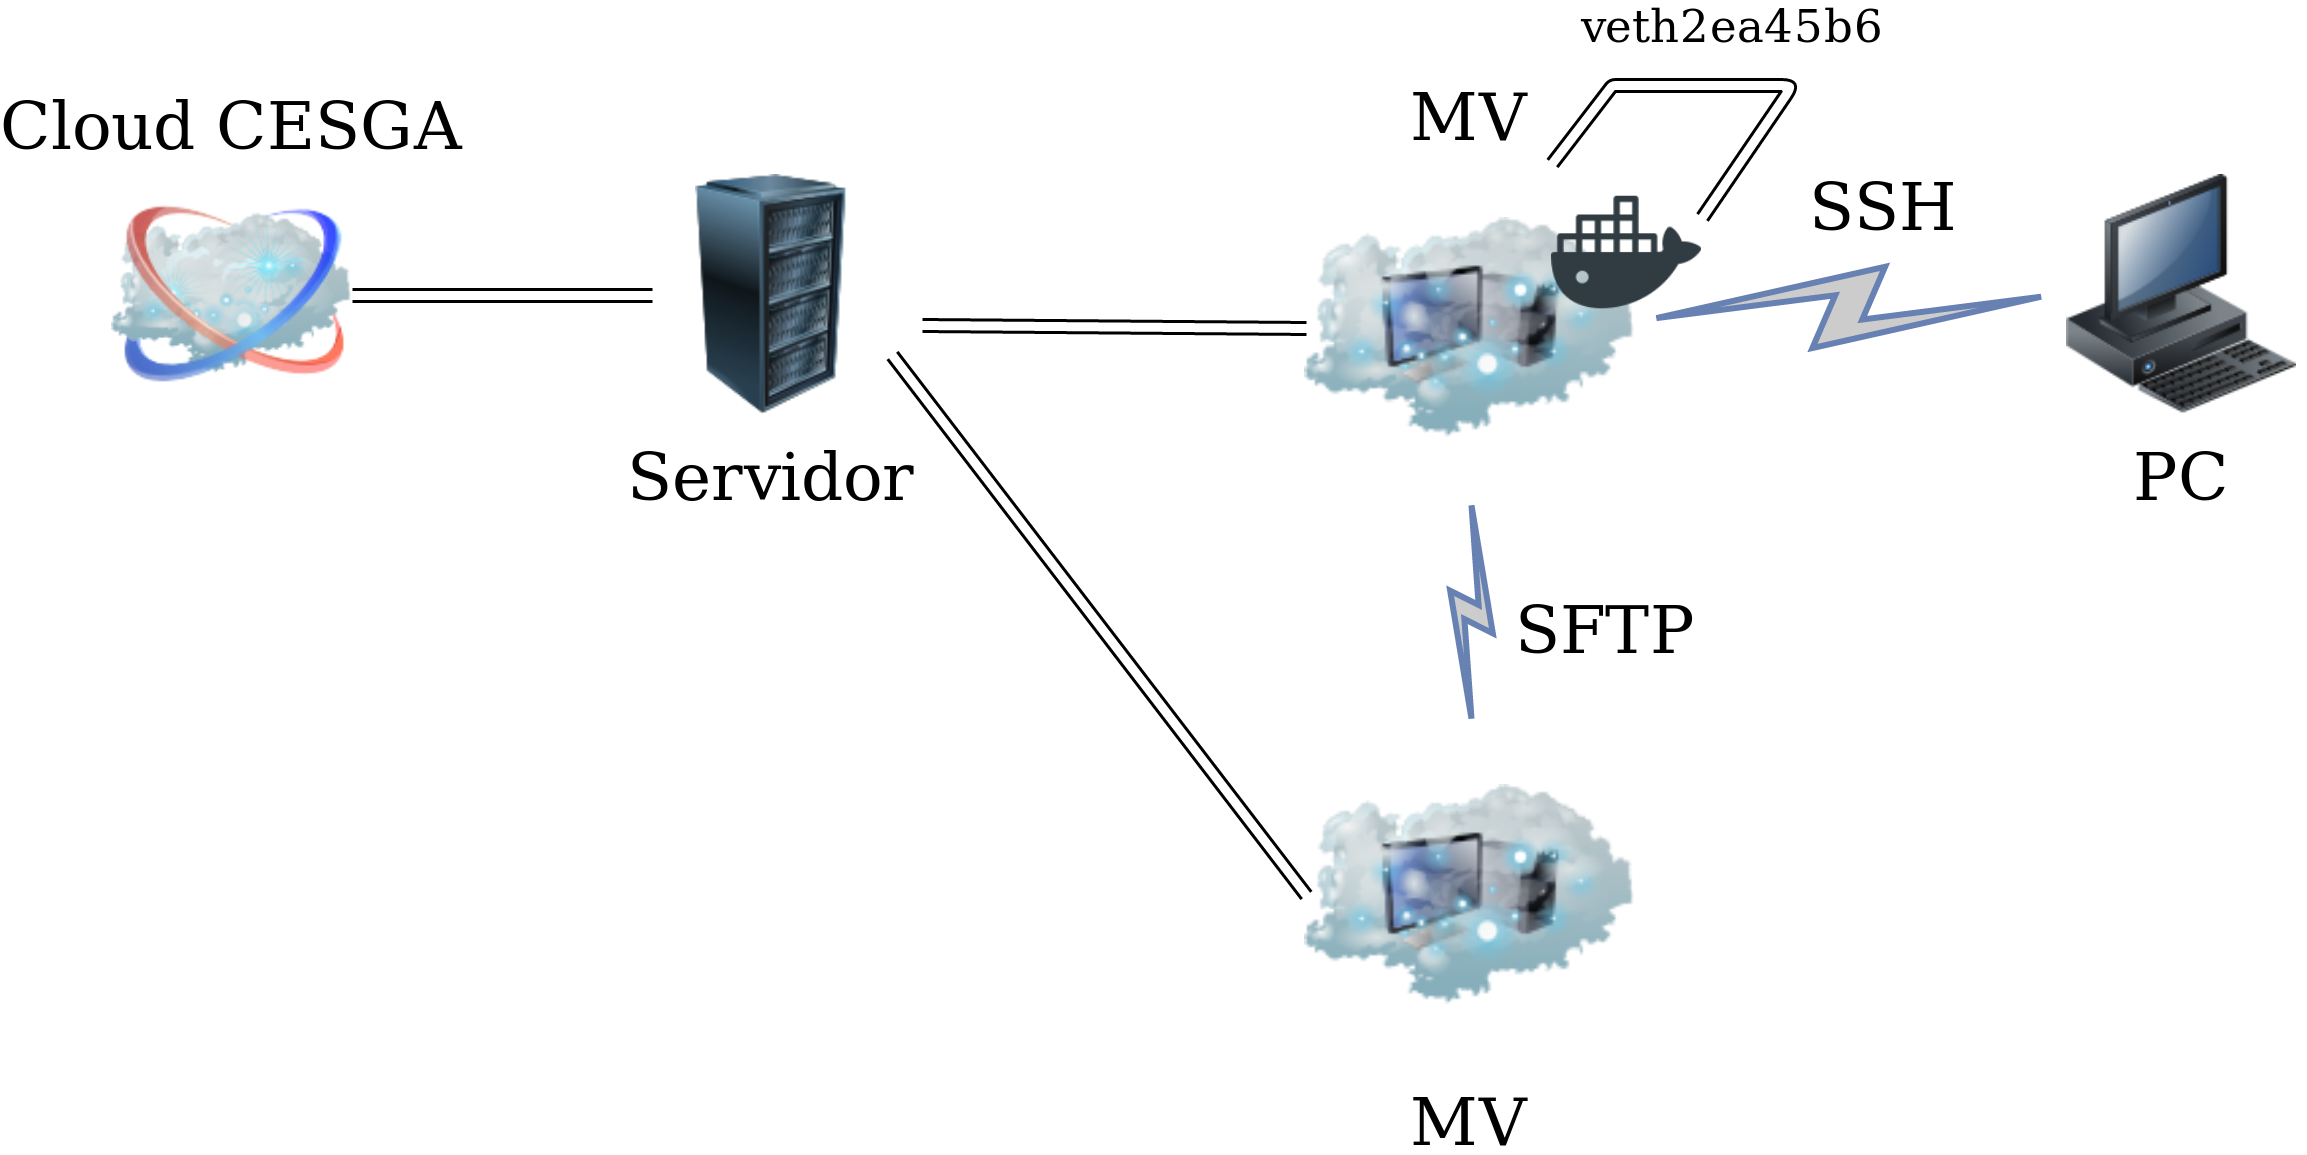
\includegraphics[width=15cm]{figuras/DiagramaQoSRedeDocker.png}}
\caption{Estrutura do despregue da QoS da rede con contedores Docker}
\label{DiagramaQoSRedeDocker}
\end{figure}

Para a realización da proba, efectuouse o envío do arquivo nun primeiro intre sen limitación algunha e logo con limitacións sobre a interface de rede do contedor empregado.\\

\begin{lstlisting}[,caption={Envío SFTP sen limitacións}]
sftp> put photo.jpg 
Uploading photo.jpg to /home/user1/photo.jpg
photo.jpg                                100% 6109KB   6.0MB/s   00:00 
\end{lstlisting}

\begin{lstlisting}[,caption={Envío SFTP con limitacións sobre o interface \textit{bridge} de Docker}]
sftp> put photo.jpg
Uploading photo.jpg to /home/user1/photo.jpg
photo.jpg                               15%  960KB   0.0KB/s - stalled -
\end{lstlisting}

Realizadas as probas pódese ver como, unha vez aplicadas as limitacións de rede, o tráfico saínte excede o máximo permitido e a transferencia non pode ser, por tanto, completada. É dicir, as limitacións aplicáronse correctamente.

\subsubsection{Probas de limitación de rede con Singularity}

No caso dos contedores Singularity, o sistema de rede empregado é o da propia máquina anfitrioa, polo que para poder aplicar limitacións farémolo sobre usuarios concretos. Deste xeito, o conxunto de contedores lanzados por un usuario soamente poderán empregar unhas características reducidas da rede segundo o criterio que o administrador de rede desexe seguir.\\

Para facer unha aproximación práctica das limitacións de rede que se queren acadar, realizarase unha proba de concepto na que se limitará a velocidade do tráfico de saída de certos usuarios.\\

Concretamente, na proba a realizar, axuntarase unha disciplina de cola directamente á raíz ({\it root}) do dispositivo. A disciplina a empregar será {\it prio}, unha disciplina moi simple que contén un número arbitrario de clases con distinta prioridade. Posto que se trata dunha proba de concepto e non dun caso real, con dúas clases bastaríanos; mais o número de clases mínimo permitido é tres. Estas clases serán creadas automaticamente, ao establecer a disciplina {\it prio}, polo que non fará falla crealas explicitamente. Ademais, a estas clases seranlle establecidas unhas disciplinas de colas sen clases (\textit{qdisc} secundarias) para marcar filtros, neste caso baseados en marcas colocadas mediante \textit{iptables}. Estas últimas disciplinas foron de tipo {\it tbf}, as cales deixan pasar paquetes até unha determinada taxa, pero coa posibilidade de aceptar refachos curtos que excedan ese límite. No referente ás limitacións establecidas, as colas terán un máximo de 1514 bytes e o tamaño dos refachos será de 1514 tamén. Para un dos usuarios limitados establecerase  unha taxa de saída de 40 kbps e para o segundo, 10 kbps. O esquema seguido pode ser apreciado na figura \ref{qdiscSingularity}, e o código asociado, no apéndice \ref{scriptQoSSingularity}. \\

\begin{figure}
\centerline{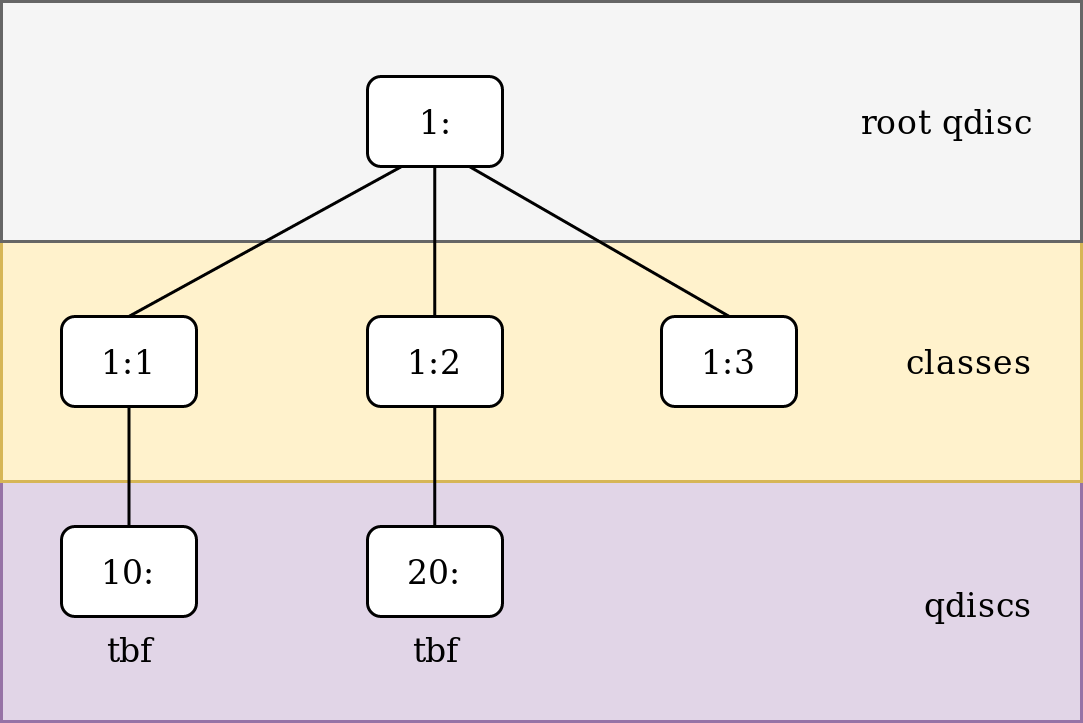
\includegraphics[width=15cm]{figuras/qdiscSingularity.png}}
\caption{Esquema da QoS da rede mediante {\it tc} en contedores Singularity}
\label{qdiscSingularity}
\end{figure}

Unha vez acadado o proceso a seguir para establecer as limitacións externas da rede segundo unha diferenciación mediante usuarios, realizouse a proba pertinente. Despegáronse dúas máquinas virtuais sobre o servizo de computación na nube do \gls{CESGA} correndo Ubuntu Xenial 16.04. Sobre unha destas máquinas aplicáronse as regras dadas no código do apéndice \ref{scriptQoSSingularity} e instalouse a tecnoloxía de contedorización Singularity. Aplicadas as limitacións pertinentes, efectuouse unha conexión \gls{SFTP} cara a segunda máquina virtual despregada, e procedeuse á transferencia dun arquivo de 5MB, coa que foi posíbel visualizar o correcto establecemento dos límites. O esquema da estrutura despregada pode ser observado na figura \ref{DiagramaQoSRedeSingularity}.\\

\begin{figure}
\centerline{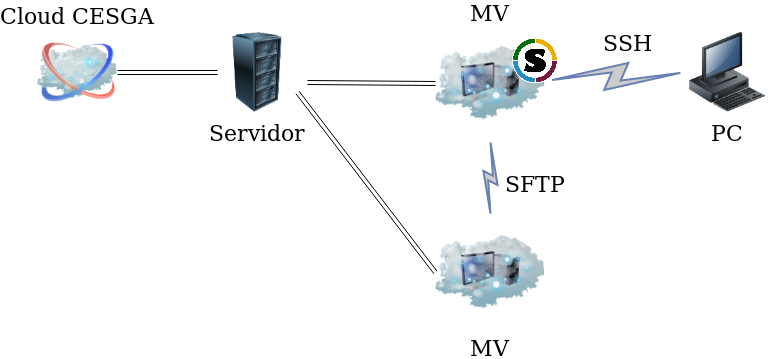
\includegraphics[width=15cm]{figuras/DiagramaQoSRedeSingularity.png}}
\caption{Estrutura do despregue da QoS da rede con contedores Singularity}
\label{DiagramaQoSRedeSingularity}
\end{figure}

A proba da transferencia realizouse como superusuario, o cal non tiña ningunha restrición, e como \textit{user1}, o cal si posuía un límite dado. Realizada a proba, as diferenzas e limitacións quedaron demostradas.

\begin{lstlisting}[,caption={Envío SFTP como superusurio}]
root@localhost:/home# singularity shell ubuntu_latest.img 
Singularity: Invoking an interactive shell within container...

Singularity ubuntu_latest.img:/home> sftp user2@10.38.3.5
user2@10.38.3.5's password: 
Connected to 10.38.3.5.
sftp> put photo.jpg 
Uploading photo.jpg to /home/user2/photo.jpg
photo.jpg                                100% 5082KB   5.0MB/s   00:00    
\end{lstlisting}

\begin{lstlisting}[,caption={Envío SFTP como \textit{user1}}]
user1@localhost:/home$ singularity shell ubuntu_latest.img
Singularity: Invoking an interactive shell within container...

Singularity ubuntu_latest.img:/home> sftp user2@10.38.3.5
user2@10.38.3.5's password: 
Connected to 10.38.3.5.
sftp> put photo.jpg 
Uploading photo.jpg to /home/user2/photo.jpg
photo.jpg                                100% 5082KB   3.9KB/s   21:38
\end{lstlisting}

Como se pode apreciar, a transferencia efectuada como superusuario realizouse coa maior celeridade posíbel, enviándose de forma practicamente instantánea. Porén, cando repetimos o envío como o usuario \textit{user1}, pódese ver como as limitacións entran en xogo e esta tarda numerosos minutos en completarse, presentando unha taxa de transferencia incluso menor á indicada.

\cleardoublepage
\chapter{Escalada de privilexios}
\minitoc
\clearpage

\section{Introdución}

Neste capítulo trataremos sobre cuestións relativas á escalada de privilexios dende os contedores, sendo a premisa unha posíbel execución de código de superusuario dende un contedor non autorizado para isto. Ao tratar cun sistema multiusuario, isto podería ter consecuencias moi graves, dende a alteración non lexítima dunha execución ata o roubo de información confidencial doutro usuario. De acadar éxito un tipo de ataque coma este nun centro coas características do \gls{CESGA}, podería ter consecuencias nefastas. Por exemplo, se mediante unha escalada un usuario non desexado obtén permisos de superusuario podería alterar ou eliminar información pertencente a un gran número de usuarios e alterar o desenvolvemento da comunidade científica que fai uso dos seus sistemas.

\section{Docker}

Cando tratamos de realizar probas de escalada de privilexios, existen moitos xeitos de abordalas, o que implica gran variabilidade destas probas segundo a configuración sistema, a versión concreta do programa a explotar, etc. Tamén debemos ter en conta que, polo de agora, non está instalada a tecnoloxía de contedorización Docker no \gls{FT2}, o que nos impide actuar con certeza sobre unha versión concreta da mesma. Estes factores, engadindo que se tratan de probas complexas, fan que realizar un estudo de posíbeis escaladas de usuario dende contedores Docker sexa unha labor complicada e gran consumidora de tempo. Debido a estas limitacións, decidiuse deixar fóra do alcance do proxecto ditas probas, xa que non serían abordábeis coas fortes limitacións de tempo ás que se afronta este proxecto.

\section{Singularity}
\label{demo-fail-escalada}

Para comprobar que o fluxo de execución de Singularity funciona correctamente, permitindo soamente a execución segundo os permisos do usuario que executou o contedor (é dicir, que o usuario que eras fóra é o mesmo que es dentro do contedor), tratarase de executar un \textit{script} propiedade de \textit{root} co \textit{setuid} activado.\\

Seguindo a lóxica de execución e permisos en sistemas GNU/Linux, o executábel debería lanzarse coma se fose \textit{root} quen o invocara, xa que esta é a propiedade que outorga o \textit{setuid}. Non obstante, segundo o explicado con anterioridade, Singularity debería impedir unha escalada de privilexios coma esta, e executar o programa cos permisos habituais do usuario, ignorando así o \textit{setuid}.\\

O executábel escollido é un programa \textit{sniffer} de paquetes en rede escrito en C con \textit{sockets raw}, cuxo código pode ser consultado no anexo \ref{esnifador}. O motivo para a escolla deste tipo de programa é que para a emprega de \textit{sockets raw} son precisos permisos de superusuario, ademais de que de ser quen de executar dito programa, suporía unha falla importante na seguridade xa que permitiría a un usuario normal facer escoita dos paquetes que transcorren pola rede. A comprobación realizouse da seguinte maneira:

\begin{enumerate}
\item Modificación dos permisos para habilitar a execución coma superusuario do executábel.

\begin{lstlisting}[]
chmod 4755 sniffer
\end{lstlisting}

\item Execución dende fóra do contedor coma usuario sen permisos de \textit{root}.

A execución foi adecuada e o programa funcionou con normalidade, permitindo a súa execución con permisos de superusuario e consentindo así a captura de paquetes da rede.

\item Execución dende dentro dun contedor.

Neste caso, o programa non acada executar coma superusuario, non tendo por tanto acceso aos \textit{sockets raw} e impedindo así súa execución.

\begin{lstlisting}[]
./sniffer eth0
Error al crear sockets: Operation not permitted
\end{lstlisting}

Queda por tanto, probado o feito de que a tecnoloxía de contedorización Singularity evita dun xeito adecuado a execución de novos procesos co \textit{setuid} activado, unha vez o contedor foi levantado no sistema.

\end{enumerate}

\section{Udocker}

Debido a que Udocker é unha ferramenta que xamais obtén nin precisa de privilexios de superusuario, resulta extremadamente complexo que sexa posíbel realizar unha escalada de privilexios dende a mesma. Polo tanto, este caso de estudo queda descartado.
\cleardoublepage
\chapter{Propostas para a mellora da seguridade}
\minitoc
\clearpage

\section{Contedores correndo sobre \gls{MV}s}

As \gls{MV}s son consideradas máis seguras que os contedores xa que engaden unha capa extra de illamento entre as aplicacións e a máquina anfitrioa. Unha aplicación correndo dentro dunha \gls{MV}, soamente é quen de comunicarse co \textit{kernel} da propia \gls{MV}, mais non co \textit{kernel} da máquina anfitrioa \cite{Securing-Docker-Containers-from-Denial-of-Service}. Amais, unha vez comprometido o \textit{kernel} da máquina virtual, tamén habería que conseguir traspasar a capa que supón o hipervisor, constituíndo un modelo con dúas capas extra de seguridade en comparativa cos contedores \cite{state-of-art-docker-security}.\\

Pola contra, os contedores pódense comunicar directamente co \textit{kernel} da máquina anfitrioa, permitindo así a un posíbel atacante gañar enormes privilexios na mesma se o seu ataque ten éxito.\\

Un posíbel fornecemento da seguridade do sistema podería pasar pola emprega dun sistema híbrido no que se despregaran contedores nunha \gls{MV}. Deste xeito, un grupo enteiro de servizos quedarían illados dos outros, ao estaren executándose dentro de dita \gls{MV}. Así, os contedores contarían coas capas extra de seguridade aportadas polas \gls{MV}s, comunicándose co seu \textit{kernel} e non directamente co \textit{kernel} da máquina anfitrioa. En troques, perderíamos a eficiencia que estes nos aportan, aínda que manteríamos intactas as súas cualidades de despregamento lixeiro e portabilidade. Outra característica moi a ter en conta no entorno no que se desenvolve este traballo é a posibilidade de continuar empregando eficientemente servizos de computación de alta prestacións, como a utilización total da memoria ou da CPU, a emprega da rede InfiniBand ou da GPU, servizos hardware aos que non se pode ter acceso directo coa emprega de \gls{MV}s.

\section{Aplicación de capas externas de seguridade}

Ademais das características de seguridade xa implantadas polas propias tecnoloxías de contedorización, ou que relegan en capacidades do \textit{kernel} de Linux, é posíbel engadir unha capa extra de seguridade empregando sistemas ben coñecidos enfocados na seguridade e con compatibilidade con contedores. Por exemplo, podemos facer emprega de mecanismos de control de acceso como o modelo discrecional, \textit{Discretionary Access Control} (DAC), ou o obrigatorio, \textit{Mandatory Access Control} (\gls{MACC}).\\

Facendo unha breve introdución, a misión dos controis de acceso é asegurar que os usuarios correctos posúen os privilexios adecuados, para o que fan uso de suxeitos, obxectos e privilexios.

\subsection{Modelo centralizado: \gls{MACC} e \gls{SELinux}}

\gls{MACC} constitúe unha implantación dun mecanismo de control de acceso obrigatorio (\gls{MACC}), Seguridade de múltiples niveis e seguridade de múltiples categorías (MLS) no \textit{kernel} de Linux. O proxecto \textit{sVirt} baséase en \gls{SELinux} e intégrase con Libvirt para provir unha separación segura para os contedores, xa que evita que os procesos raíz dentro dun contedor infiran cos procesos que se executan fóra deste contedor. \cite{Securing-Docker-Containers-from-Denial-of-Service}\\

Este modelo basea o seu funcionamento en políticas do sistema que non poden ser alteradas por usuarios individuais. Neste modelo, os obxectos inclúen un nivel de seguridade e un conxunto de categorías, mentres que os usuarios posúen permisos para cada clase. Deste xeito, existen regras baseadas en clases de acceso e autorización para administrar a lectura e escritura de obxectos. \\

Co fin de reducir a exposición de seguridade e cumprir co principio do mínimo privilexio, moitos sistemas operativos proporcionan un sistema \gls{MACC} integrado. Os \gls{MACC} poden ser empregados para fornecer o illamento entre os diferentes contedores e a máquina anfitrioa, así como para cumprir as políticas dos procesos executados dentro dos contedores \cite{OS-level-security}. Dita característica está completamente integrada no \textit{kernel}, mais debido ás complexas regras que o conforman, pode ser difícil de configurar. Algunhas das solucións máis comúns para a súa emprega son AppArmor e \gls{SELinux} \cite{TFM}.\\

Nos sistemas que empregan \gls{SELinux}, Docker aproveita a política definida no proxecto \textit{sVirt}, no que se apuntan políticas de seguridade para diferentes modelos de virtualización. Existen dúas maneiras de separar os procesos en \gls{SELinux}:

\begin{enumerate}
    \item \textit{Type Enforcement} (TE): unha etiqueta que contén un tipo está asociada a cada suxeito (proceso) e obxecto do sistema (ficheiro e directorio). A política define as accións permitidas entre os tipos e o \textit{kernel} impón estritamente estas regras. Docker asigna unha etiqueta cun conxunto reducido de privilexios a todos os procesos que se executan en contedores. TE emprégase para protexer o motor de Docker e a máquina anfitrioa dos contedores, que poden provir de fontes que non sexan de confianza.
    
    \item \textit{Multi-Category Secutiry} (MCS): a etiqueta asignada ao suxeito ou obxecto pódese subdividir con múltiples categorías para crear instancias diferentes do mesmo tipo. Acéptase unha solicitude de acceso se TE o permite primeiro e o suxeito e o obxecto están na mesma categoría. Non obstante, é vantaxoso se se asignan diferentes categorías a diferentes contedores para que teñan unha separación clara entre si.
\end{enumerate}

Podemos concluír que \gls{SELinux} supón unha capa engadida de seguridade que protexe o sistema da máquina anfitrioa, polo que no caso de que un ataque tivese éxito no interior dun contedor e conseguise acceder á propia máquina anfitrioa, \gls{SELinux} interviría para frustrar o ataque. Se un proceso de dentro do contedor consegue obter acceso a un arquivo da máquina anfitrioa e tenta facer operación de lectura ou escritura, \gls{SELinux} encargarase antes de verificar o seu acceso, impedindo o ataque ao detectar a falta de tales privilexios. \cite{SELinuxMitigates}

\section{Actualización do sistema}
\label{actualizacionSistema}

Unha das premisas máis importantes no eido da seguridade parte de manter o noso sistema ao día, para obter os parches de seguridade actuais e pór solución a un gran número de vulnerabilidades. Cando traballamos con contedores, esta premisa mantense presente, e grazas á flexibilidade que estes nos outorgan, debemos manter sempre o sistema actualizado para diminuír o número de vulnerabilidades que poidan conter.\\

Para evidenciar tal afirmación, realizarase unha proba con contedores Docker e Clair. O desenvolvemento esperado da proba é o seguinte:

\begin{enumerate}
    \item Descarga dunha imaxe dun contedor dende o Docker Hub.
    \item Exploración do número de vulnerabilidades existentes en dita imaxe coa axuda de Clair.
    \item Creación dun repositorio propio no Docker Hub, onde se almacenará unha imaxe derivada da imaxe orixinal.
    \item Actualización do sistema atopado no contedor, coa axuda do xestor de paquetes \gls{APT}.
    \item Creación da imaxe derivada, mediante a realización dun \textit{commit} sobre o contedor coas actualizacións xa efectuadas.
    \item Exploración do número de vulnerabilidades existentes na imaxe derivada e actualizada.
\end{enumerate}

Posto que xa existen imaxes no sistema, será empregada unha delas. Concretamente será empregada unha imaxe de MongoDB. Se comezamos facendo a primeira análise con \textit{clair-scanner} (figura \ref{rep1}), vemos como atopamos en primeira instancia 73 vulnerabilidades. Posteriormente realizamos o proceso de inicio de sesión no Docker Hub (figura \ref{rep3}), no cal xa existirá un repositorio creado para o almacenamento da imaxe que imos formar a partir da imaxe de MongoDB oficial. Continuaremos coa actualización dos paquetes mediante \gls{APT} (figura \ref{rep4}). Tendo xa un contedor actualizado, realizaremos un \textit{commit} deste sobre a nosa propia imaxe (figura \ref{rep5}). Para rematar, invocamos novamente á ferramenta \textit{clair-scanner}, mais está vez para que realice unha análise de vulnerabilidades sobre a imaxe derivada que acabamos de formar (figura \ref{rep2}). Desta segunda volta, a ferramenta detecta 66 vulnerabilidades, é dicir 7 vulnerabilidades menos no sistema con tan só realizar unha simple actualización. Queda por tanto, probada a importancia de manter o noso sistema ao día. Ademais, é probábel que se entramos nun estudo máis minucioso sexa posíbel reducir aínda máis o número de vulnerabilidades, por exemplo, eliminando librarías innecesarias, e conseguir así un sistema máis seguro.

\begin{figure}
\centerline{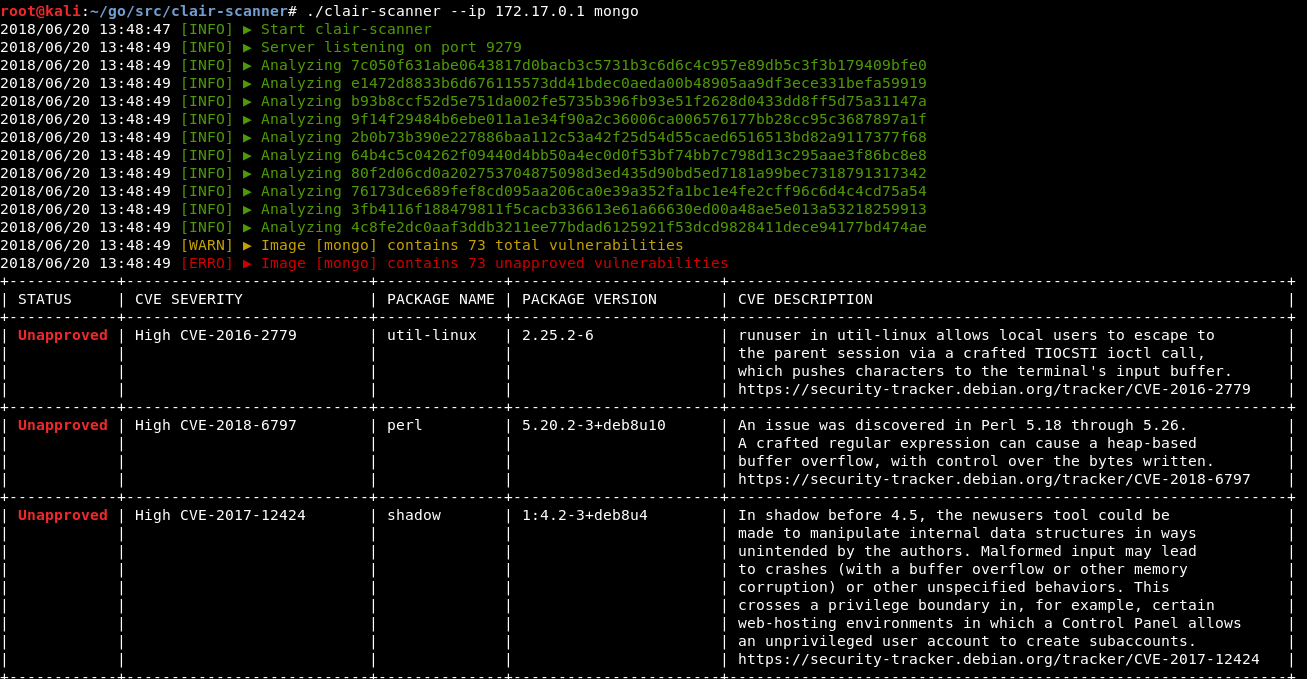
\includegraphics[width=15cm]{figuras/rep1.png}}
\caption{Escáner coa ferramenta \textit{clair-scanner} dunha imaxe de MongoDB}
\label{rep1}
\end{figure}

\begin{figure}
\centerline{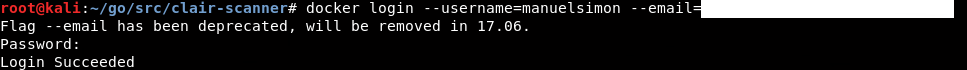
\includegraphics[width=15cm]{figuras/rep3.png}}
\caption{Inicio de sesión no Docker Hub}
\label{rep3}
\end{figure}

\begin{figure}
\centerline{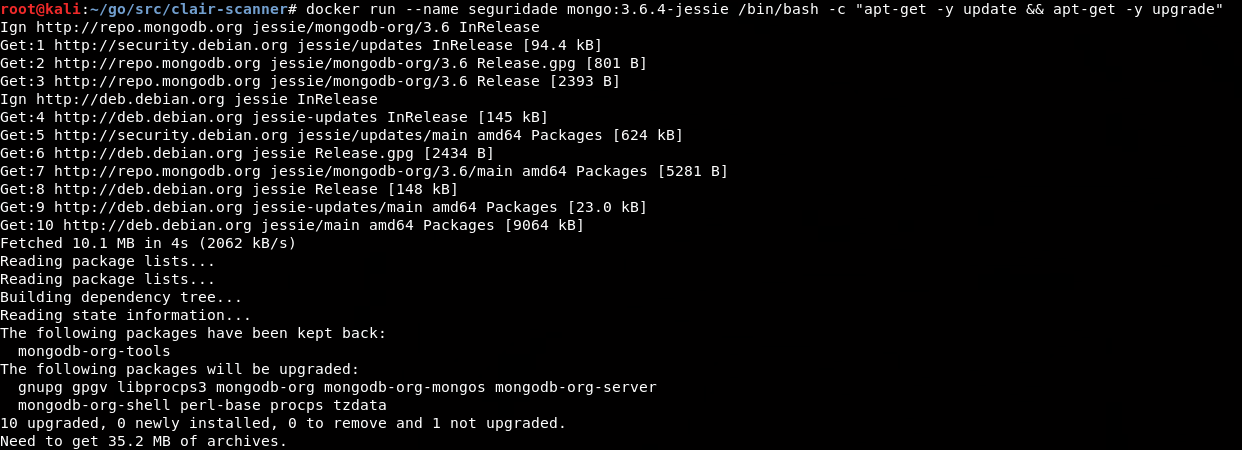
\includegraphics[width=15cm]{figuras/rep4.png}}
\caption{Execución do contedor ``seguridade'' a partir dunha imaxe de MongoDB e actualización dos paquetes}
\label{rep4}
\end{figure}

\begin{figure}
\centerline{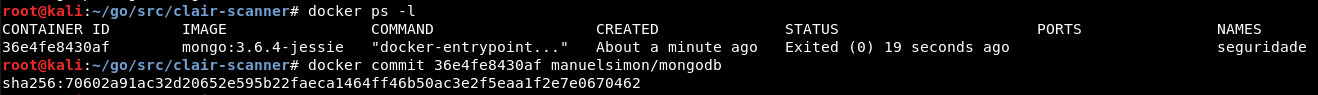
\includegraphics[width=15cm]{figuras/rep5.png}}
\caption{Execución de \textit{commit} do contedor ``seguridade'' sobre a nosa propia imaxe}
\label{rep5}
\end{figure}

\begin{figure}
\centerline{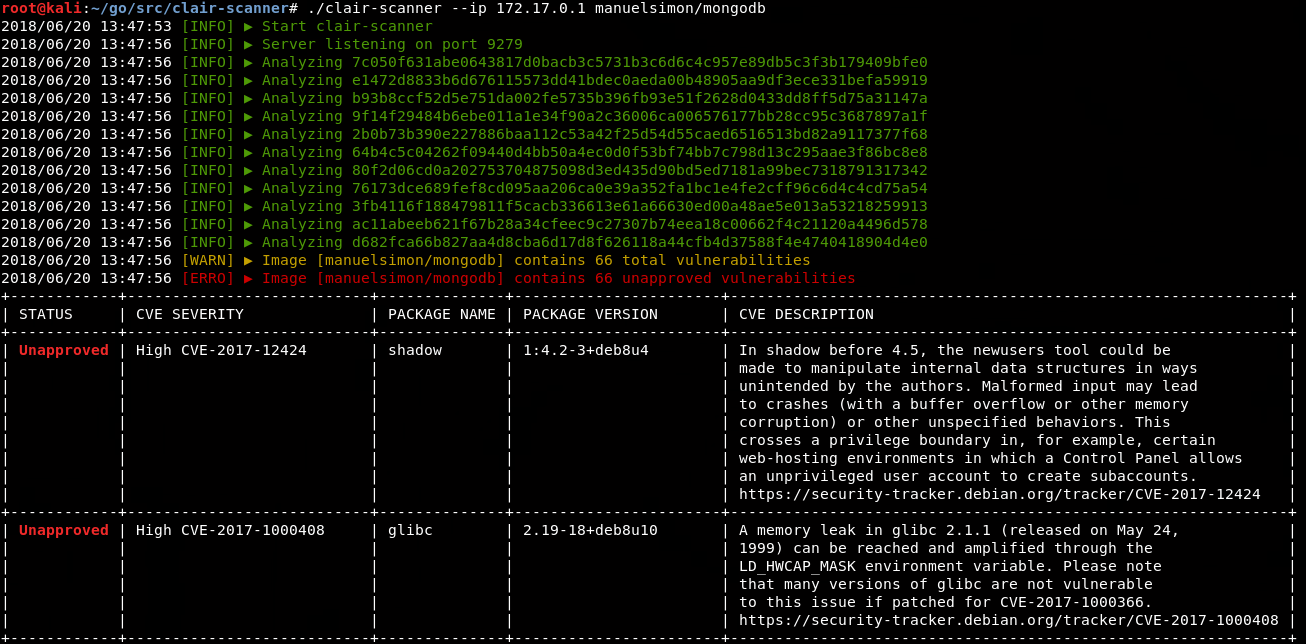
\includegraphics[width=15cm]{figuras/rep2.png}}
\caption{Escáner coa ferramenta \textit{clair-scanner} da imaxe actualizada de MongoDB}
\label{rep2}
\end{figure}

\section{Auditoría do sistema}

A auditoría informática é un proceso que consiste en recoller, agrupar e avaliar evidencias para determinar se un sistema posúe un nivel de seguridade adecuado, ou leva a cabo eficazmente os fins da organización, empregando eficientemente os recursos e cumprindo as leis e regulacións establecidas. A medida que as tecnoloxías de contedorización se van facendo un oco na industria, aparecen cada vez máis medidas reguladoras para a súa correcta utilización.\\

\subsection{\textit{Docker Bench Audit Tool}}
\label{DockerBeckAuditTool}

No eido da auditoría de seguridade na emprega de contedores podémonos atopar coa ferramenta \textit{Docker Bench Audit Tool}, facilitada polos propios desenvolvedores de Docker. Esta ferramenta trátase dunha serie de comandos que procura entre ducias de boas prácticas comúns no referente á implantación de contedores Docker. Tales probas son de dominio público e calquera pode revisalas, de xeito que se procura a implantación dun método doado de realizar a auditoría de seguridade dos sistemas coa tecnoloxía de contedorización Docker. \cite{docker-bench-security} \\

A figura \ref{dockerBench} amosa unha execución de dita ferramenta sobre o equipo local de desenvolvemento. Non é posíbel executar dita ferramenta de auditoría directamente sobre o \gls{FT2} posto que a tecnoloxía de contedorización de Docker aínda non está configurada no sistema. Podemos observar como a información é clasificada en diferentes niveis, segundo superaran as probas de auditoría ou non. Por exemplo, é posíbel comprobar como o espazo de nomes para os usuarios non están activados, o que implicaría que de ocorrer unha escalada de privilexios neste sistema, o atacante tería os mesmos privilexios fóra que dentro do contedor.

\begin{figure}
\centerline{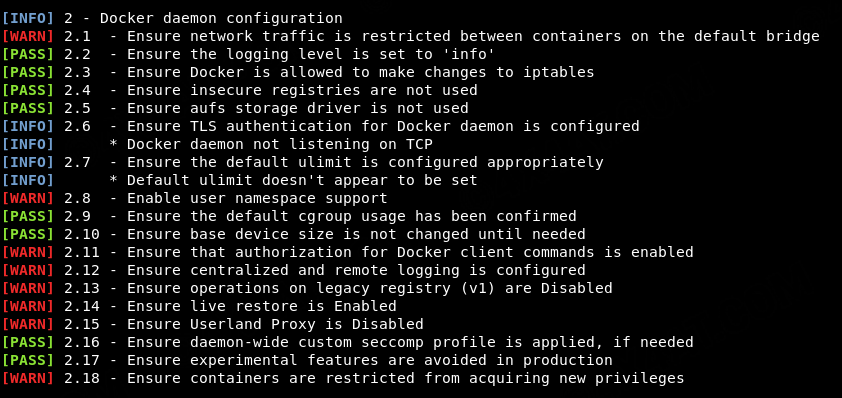
\includegraphics[width=15cm]{figuras/dockerBench.png}}
\caption{Saída parcial da execución da ferramenta \textit{Docker bench tool}}
\label{dockerBench}
\end{figure}


\section{Boas prácticas}

Hai unha serie de boas prácticas na emprega e configuración de entornos baseados en contedores aceptados pola industria. Moitos deles xa foron abordados ao longo deste documento, como poden ser:

\begin{itemize}
    \item \textbf{Principio de manter só o esencial:} cómpre reducir o número de binarios e servizos correndo dentro dos contedores, reducindo así as posibilidades de que un ataque teña lugar, ao limitar o número de vulnerabilidades existentes dentro dos contedores. Se queremos coñecer os paquetes instalados e o seu estado, podemos facer emprega de xestores de paquetes como poden ser {\tt dpkg}, tal e como amosa a figura \ref{dpkgl}.
    
    \begin{figure}
    \centerline{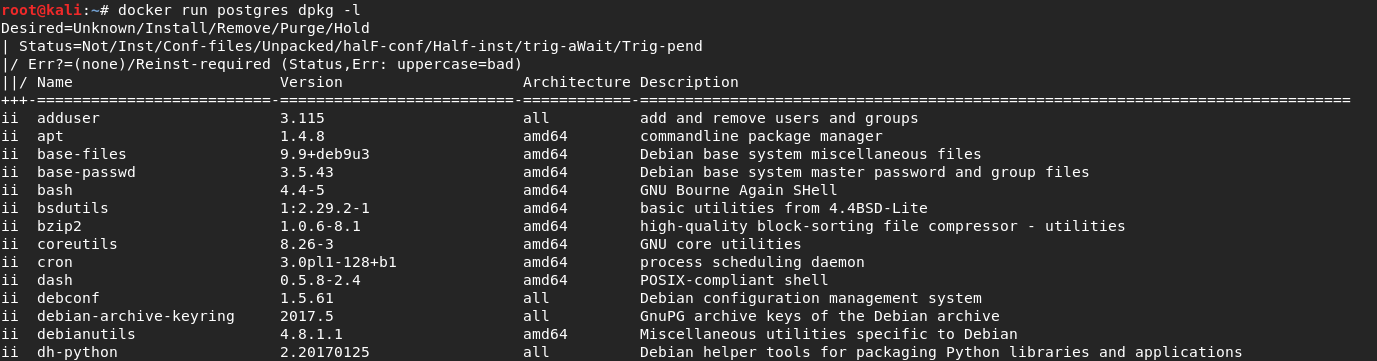
\includegraphics[width=15cm]{figuras/dpkgl.png}}
    \caption{Mostra de paquetes e versións nun contedor Docker con PostgreSQL 9.6}
    \label{dpkgl}
    \end{figure}
    
    \item \textbf{Empregar sistema de só lectura:} os sistemas de ficheiros son unha importante fonte de ataque por parte dos intrusos non desexados. Empregando un sistema de só lectura dentro dos contedores é posíbel parar certos tipos de ataques, como a subida de scripts maliciosos ou a sobreescritura de datos sensíbeis. Sempre que sexa posíbel, debemos empregar sistemas de só lectura nos contedores. Isto tamén é aplicábel aos volumes externos aos que estean conectados os contedores.
    
    \begin{lstlisting}[,caption={Proba de escritura en contedor de só lectura}]
docker run --read-only ubuntu touch proba
touch: cannot touch 'proba': Read-only file system
    \end{lstlisting}
    
    \begin{lstlisting}[,caption={Proba de escritura en sistema compartido de só lectura}]
docker run -v /root/Downloads/:/Downloads:ro ubuntu touch /Downloads/proba2
touch: cannot touch '/Downloads/proba2': Read-only file system
    \end{lstlisting}
    
    \item \textbf{Limitar as chamadas ao \textit{kernel}:} posto que contedores e máquina anfitrioa comparten \textit{kernel}, esta resulta unha proposta moi interesante, posto que un ataque exitoso sobre o \textit{kernel} do sistema podería ter serias implicacións non soamente no propio contedor, senón tamén noutros contedores e na propia máquina anfitrioa. Unha posíbel solución podería pasar pola emprega de sistemas enfocados na seguridade como \gls{SELinux}, nos que é posíbel limitar as chamadas ao sistema que un contedor pode facer.
    
    \item \textbf{Limitar os recursos:} para evitar posíbeis ataques de denegación de servizo é importante limitar os recursos que un contedor pode empregar. Estas limitacións poder vir dadas pola propia tecnoloxía de contedorización ou facer uso de sistemas externos baixo diversos criterios de clasificación.
    
    \item \textbf{Reducir as vulnerabilidades existentes nas imaxes:} coa a axuda de ferramentas externas é posíbel descubrir as vulnerabilidades que posúen as imaxes dos nosos contedores. Tendo coñecemento das mesmas podemos aplicar medidas para reducilas, por exemplo actualizando á última versión as librarías a empregar.
    
    \item \textbf{Manter actualizadas as tecnoloxías de virtualización:} a medida que as tecnoloxías de virtualización actualízanse incorporan novas e mellores medidas de seguridade. É importante manter o sistema actualizado para obter ditas melloras, sobre todo cando é lanzada algunha versión enfocada na revisión da seguridade do sistema, como supuxo Docker 1.10 coa introdución de espazos de nomes para usuarios.
    
    \item \textbf{Tratamento adecuado de información confidencial:} cando traballamos con certas aplicacións é posíbel que precisen facer uso de información confidencial, tal como contrasinais (por exemplo, para realizar accesos a bases de datos). Se un atacante logra ter acceso a esta información, tamén gañará o acceso a estes servizos, polo que é importante manter segura esta información. Debemos evitar facer emprega das variábeis de entorno para almacenar esta información, xa que son doadamente accesíbeis e amplamente empregadas. No seu canto, esta información pode ser almacenada en ficheiros no interior de volumes externos aos que só o usuario adecuado teña permisos de acceso. Para incrementar a seguridade, ditos volumes deberían ser de só lectura, evitando que alguén puidera modificar dita información.
    
    \item \textbf{Non dar acceso a directorios perigosos da máquina anfitrioa:} algúns contedores precisaran acceso a directorios especiais como {\tt /proc}, {\tt /dev}, etc. Normalmente, estas montaxes son precisas para realizar algunha funcionalidade especial do contedor, non obstante, debemos asegurarnos de comprender por que e como certos procesos queren acceder a información privilexiada. Habitualmente, expor estas rutas privilexiadas con permisos de só lectura debería abondar, polo que non debemos outorgar privilexios de escritura sen nos preguntar por que.
    
    \item \textbf{Configurar ferramentas de xestión de \gls{OOM}:} para evitar posíbeis ataques de denegación de servizo, podemos facer uso de ferramentas que eviten a sobreemprega destes recursos do sistema, como pode ser a memoria. Algunhas tecnoloxías, como Docker, xa incorporan o seu propio ``\gls{OOM} \textit{killer}'', mais existe a posibilidade de configurar un xestor externo.
    
    \item \textbf{Configurar o \textit{socket} de Docker de xeito seguro se é precisa unha conexión en rede:} por defecto, Docker execútase a través dun \textit{socket} Unix non conectado á rede, pero tamén é posíbel empregar un socket HTTP no caso de querer que dita tecnoloxía funcione en rede. Neste caso, é preciso configurar unha serie de parámetros se queremos que a emprega de Docker en rede sexa segura, como a habilitación de TLS ou a configuración de certificados.
    
    \item \textbf{Establecer un sistema de detección de vulnerabilidades en imaxes:} cando traballamos con imaxes provintes de diferentes fontes corremos o risco de despregar sistemas que conteñan vulnerabilidades. Para miniaturizar este risco e coñecer o estado ao que pasará o noso sistema de despregar tales imaxes podemos facer uso de ferramentas que permiten a detección de vulnerabilidades. Estas ferramentas permitirán a identificación de vulnerabilidades antes de que o sistema sexa despregado, outorgándonos gran cantidade de información, segundo a cal poderemos actuar. Existen incluso ferramentas que se poden integrar nun proceso de despregamento no que non se permita a instanciación de contedores que conteñan certas vulnerabilidades.
    
    \item \textbf{Empregar mecanismos de validación de imaxes:} todas as tecnoloxías de contedorización estudadas posúen mecanismos para a validación das imaxes, conseguindo aumentar a seguridade do sistema ao permitirnos tratar só con imaxes fiábeis. Deberiamos empregar soamente aquelas imaxes cuxa procedencia sexa coñecida e fiábel.
    
    \item \textbf{Empregar mecanismos externos de seguridade:} a seguridade por capas é unha das mellores solucións que existen, posto que se unha das capas se ve comprometida, aínda existirán outras que manterán seguro ao sistema. Por isto, a emprega de solucións externas para a protección do noso sistema baseado en contedores poden ser moi interesantes. Unha das solucións externas máis soadas a día de hoxe é \gls{SELinux}.
    
    \item \textbf{Manter o sistema actualizado:} para obter as últimas actualizacións de seguridade cómpre manter o noso sistema ao día na medida en que isto sexa posíbel. Esta actualización afecta tanto á máquina anfitrioa como ao sistema interno de cada contedor individual.

\end{itemize}

%
% Engadir os capitulos que fagan falta
%
\cleardoublepage
\chapter{Conclusións e posíbeis ampliacións}
\minitoc
\clearpage

\section{Conclusións}

Ao longo deste documento foron estudadas as implicacións de seguridade na emprega de contedores nun entorno \gls{HPC}, analizando para tal fin tres das tecnoloxías de contedorización máis soadas neste eido. Amosáronse diversos puntos de falla e estudáronse as súas implicacións dun xeito teórico-práctico, evidenciando os riscos asociados a tales tecnoloxías se non son tratadas con coidado.\\

Os resultados do estudo atópanse resumidos na táboa \ref{resumoRiscosSolucions}, onde se amosan os riscos detectados así como posíbeis solucións aos mesmos. \\

\begin{table}[]
\centering
\caption{Resumo dos riscos atopados e as súas posíbeis solucións}
\label{resumoRiscosSolucions}
\resizebox{\textwidth}{!}{%
\begin{tabular}{|l|c|c|c|c|c|}
\hline
 & \begin{turn}{90} Explotación do \textit{kernel} \end{turn} & \begin{turn}{90} Ataques de \gls{DoS} \end{turn} & \begin{turn}{90} Escalada de privilexios \end{turn} & \begin{turn}{90} Vulnerabilidades en imaxes \space \end{turn} & \begin{turn}{90} Segredos comprometidos \end{turn} \\ \hline
Contedores correndo sobre \gls{MV}s & \rotatebox[origin=c]{270}{$\Lsh$} &  & \rotatebox[origin=c]{270}{$\Lsh$} &  &  \\ \hline
Limitación de recursos &  & \rotatebox[origin=c]{270}{$\Lsh$} &  &  &  \\ \hline
Validación de imaxes &  &  &  & \rotatebox[origin=c]{270}{$\Lsh$} &  \\ \hline
Emprega de sistemas de só lectura & \rotatebox[origin=c]{270}{$\Lsh$} & \rotatebox[origin=c]{270}{$\Lsh$} & \rotatebox[origin=c]{270}{$\Lsh$} &  & \rotatebox[origin=c]{270}{$\Lsh$} \\ \hline
Non empregar variábeis de entorno &  &  &  &  & \rotatebox[origin=c]{270}{$\Lsh$} \\ \hline
Non empregar o flag \textit{--privileged} & \rotatebox[origin=c]{270}{$\Lsh$} &  & \rotatebox[origin=c]{270}{$\Lsh$} &  & \rotatebox[origin=c]{270}{$\Lsh$} \\ \hline
Inhabilitar a comunicación entre contedores & \rotatebox[origin=c]{270}{$\Lsh$} & \rotatebox[origin=c]{270}{$\Lsh$} & \rotatebox[origin=c]{270}{$\Lsh$} &  &  \\ \hline
Emprega de volumes de só lectura & \rotatebox[origin=c]{270}{$\Lsh$} &  & \rotatebox[origin=c]{270}{$\Lsh$} &  &  \\ \hline
Principio de manter só o esencial & \rotatebox[origin=c]{270}{$\Lsh$} &  & \rotatebox[origin=c]{270}{$\Lsh$} &  &  \\ \hline
Limitar as chamadas ao \textit{kernel} & \rotatebox[origin=c]{270}{$\Lsh$} & \rotatebox[origin=c]{270}{$\Lsh$} &  &  &  \\ \hline
Manter actualizado o entorno &  &  & \rotatebox[origin=c]{270}{$\Lsh$} &  &  \\ \hline
Non dar acceso a directorios perigosos & \rotatebox[origin=c]{270}{$\Lsh$} &  & \rotatebox[origin=c]{270}{$\Lsh$} &  & \rotatebox[origin=c]{270}{$\Lsh$} \\ \hline
Ferramentas anti \gls{OOM} &  & \rotatebox[origin=c]{270}{$\Lsh$} &  &  &  \\ \hline
Mecanismos externos de seguridade & \rotatebox[origin=c]{270}{$\Lsh$} &  & \rotatebox[origin=c]{270}{$\Lsh$} &  &  \\ \hline
Detección de vulnerabilidades en imaxes &  &  &  & \rotatebox[origin=c]{270}{$\Lsh$} &  \\ \hline
 \end{tabular}
}
\end{table}

Grazas ao feito de empregar unha metodoloxía áxil como Scrum, o nivel de incerteza que implicaba o proxecto foi solucionado, avanzando no seu desenvolvemento a medida que o estudo permitía a obtención de novos datos e o acceso a un nivel de refinamento maior. Tentar realizar o desenvolvemento deste proxecto cunha metodoloxía tradicional resultaría moi arriscado, debido ao gran descoñecemento sobre os conceptos do estudo nun comezo. Polo tanto, podemos concluír que a elección dunha metodoloxía áxil foi adecuada e axudou ao desenvolvemento do proxecto.

\section{Traballo futuro}

Debido ás fortes limitacións temporais ás que se afrontou o proxecto, non foi posíbel realizar unha gran cantidade de probas, mais si quedaron mostradas as partes esenciais do estudo. Unha futura continuidade deste proxecto podería pasar pola realización dun maior número de probas. Outra limitación importante viu dada pola inexistencia da tecnoloxía de contedorización Docker no \gls{FT2}, un dos entornos de proba nos que se desenvolvía o proxecto. Unha vez dita tecnoloxía estea configurada no entorno, será posíbel realizar estudos máis concretos sobre a mesma. Por exemplo, a configuración do sistema atendendo ás medidas de auditoría da ferramenta \textit{Docker Bench Audit Tool}.


\cleardoublepage

% Aquí empezan os apéndices
\appendix
\cleardoublepage
\chapter{Códigos}
\minitoc
\clearpage

Códigos empregados para a realización de diferentes probas ao longo do proxecto desenvolvido.

\section{Despregamento das probas \gls{ARP} \textit{spoofing} e \gls{MAC} \textit{flooding}}
\label{codigo-arp-spoofing}

\textbf{Fonte}: propia.

\begin{lstlisting}[,caption={Arquivo docker-compose.yml empregado para a realización de probas de rede \gls{ARP} \textit{spoofing} e \gls{MAC} \textit{flooding}}]
version: "2"

services:
    nginx:
        image: nginx:latest
        command: nginx-debug -g 'daemon off;'
        volumes:
           - ./nginx/nginx.conf:/etc/nginx/nginx.conf:ro
        ports:
            - "8080:80"
    ubuntu:
        image: ubuntu:latest
        bash -c "apt-get update &&  apt-get -y install net-tools curl && apt-get clean && tail -F anything"
    kali:
        image: kalilinux/kali-linux-docker:latest
        command: bash -c "apt-get update && apt-get -y upgrade &&  apt-get -y install dnsutils net-tools dsniff iproute2 tcpdump && apt-get clean && tail -F anything"
        expose:
           - "80"
\end{lstlisting}

\section{\textit{Sniffer} de paquetes con \textit{sockets raw}}
\label{esnifador}

\textbf{Autor}: Diego Ferro

\textbf{Fonte}: \url{https://github.com/MrSegfault/sniffer\_redes}

\begin{lstlisting}[,caption={\textit{Sniffer} de paquetes con \textit{sockets raw}}]
#include<stdio.h>
#include<stdlib.h>
#include<sys/types.h>
#include<sys/socket.h>
#include<netinet/in.h>
#include<netinet/tcp.h>
#include<netinet/udp.h>
#include<netinet/ip_icmp.h>
#include<netdb.h>
#include<string.h>
#include<unistd.h>
#include<sys/ioctl.h>
#include<net/if.h>
#include<netinet/if_ether.h>

int main(int argc, char** argv){
        int s,contr;
        struct ifreq ifr;
        unsigned char buf[65536];
        unsigned int buflen=65536*sizeof(unsigned char);
        ssize_t rec;
        int i;
        gid_t gid;
        uid_t uid;

        gid = 0;
        uid = 0;

        setresgid(gid, gid, gid);
        setresuid(uid, uid, uid);

        if(argc!=2){
                printf("Numero incorrecto de argumentos\n");
                exit(1);
        }

        s=socket(AF_PACKET,SOCK_RAW,htons(ETH_P_ALL));
        contr=socket(AF_INET,SOCK_DGRAM,IPPROTO_UDP);
        if(s<0 || contr<0){
                perror("Error al crear sockets");
                exit(1);
        }
        strcpy(ifr.ifr_name,argv[1]);
        if(ioctl(contr,SIOCGIFFLAGS,&ifr)<0){
                perror("Error al conseguir estado\n");
                exit(1);
        }
        ifr.ifr_flags |= IFF_PROMISC;
        if(ioctl(contr,SIOCSIFFLAGS,&ifr)<0){
                perror("Error activando el modo promiscuo\n");
                exit(1);
        }
        while((rec=recv(s,buf,buflen,0))>0){
                for(i=0;i<rec;i++){
                        printf("%c",buf[i]);
                }
                printf("\n");
        }
        ifr.ifr_flags &= ~IFF_PROMISC;
        if(ioctl(contr,SIOCSIFFLAGS,&ifr)<0){
                perror("Error desactivando el modo promiscuo\n");
                exit(1);
        }
        close(contr);
        close(s);

        return 0;
}
\end{lstlisting}


\section{Programa consumidor de memoria}
\label{consumidorMemoria}

\textbf{Fonte}: propia.

\begin{lstlisting}[,caption={Código programa consumidor de memoria}]
#include <stdlib.h>

void f(long double *a){
	a = (long double *)malloc(sizeof(long double) * 1000);
}

int main(void) {
	long double *a;

        while(1) {
		f(a);
        }
        return 0;
}

\end{lstlisting}

\section{\gls{QoS} da rede mediante \textit{tc} en contedores Singularity}
\label{scriptQoSSingularity}

\begin{lstlisting}[,caption={Script QoS da rede mediante {\tt tc} en contedores Singularity}]
useradd -c "User 1" user1 -m -s /bin/bash
useradd -c "User 2" user2 -m -s /bin/bash
# passwd user1
# passwd user2
tc qdisc add dev eth0 root handle 1: prio
tc qdisc add dev eth0 parent 1:1 handle 10: tbf limit 1514b burst 1514b rate 40kbit
tc qdisc add dev eth0 parent 1:2 handle 20: tbf limit 1514b burst 1514b rate 10kbit
iptables -A OUTPUT -t mangle -m owner --uid-owner user1 -j MARK --set-mark 5
iptables -A OUTPUT -t mangle -m owner --uid-owner user2 -j MARK --set-mark 10
tc filter add dev eth0 parent 1:0 protocol ip prio 1 handle 5 fw flowid 1:1
tc filter add dev eth0 parent 1:0 protocol ip prio 1 handle 10 fw flowid 1:2
\end{lstlisting}


\section{\gls{QoS} da rede mediante \textit{tc} en contedores Docker}
\label{scriptQoSDocker}

\textbf{Fonte}: propia.

\begin{lstlisting}[,caption={Script QoS da rede mediante {\tt tc} en contedores Docker}]
tc qdisc add dev veth2ea45b6 root tbf rate 1024kbit latency 50ms burst 200
\end{lstlisting}


\section{Cotas de disco}
\label{scriptQuotas}

\textbf{Fonte}: propia.

\begin{lstlisting}[,caption={Cuotas de disco}]
# useradd -c "Nuevo Usuario Cuotas" nuevousuariocuotas -m -s /bin/bash -g staff
# passwd nuevousuariocuotas
apt-get install quota
echo "UUID=deb5e4ba-4656-4331-8bf2-6a3450425c3e /               ext4    defaults,usrjquota=aquota.user,grpjquota=aquota.group,jqfmt=vfsv0,errors=remount-ro   0       1" >> /etc/fstab
mount -vo remount /
quotacheck -vguma
quotaon -va
edquota -u nuevousuariocuotas -f /
    # Engadimos: /dev/vda1                      2416      10000     100000         14        0        0
\end{lstlisting}
%\cleardoublepage
%\chapter{Manuais de usuario}

Manuais de usuario: incluirán toda a información precisa para aquelas persoas que utilicen o Sistema: instalación, utilización, configuración, mensaxes de erro, etc. A documentación do usuario debe ser autocontida, é dicir, para o seu entendemento o usuario final non debe precisar da lectura de outro manual técnico.

\cleardoublepage
%\chapter{Licenza}
Se se quere pór unha licenza (GNU GPL, Creative Commons, etc), o texto da licenza vai aquí.


%\cleardoublepage
\markboth{BIBLIOGRAFÍA}{BIBLIOGRAFÍA}
\addcontentsline{toc}{chapter}{Bibliografía}


\begin{thebibliography}{99}

% EXEMPLO DE ARTIGO DE REVISTA
\bibitem{Securing-Docker-Containers-from-Denial-of-Service} J. Chelladhurai, P. R. Chelliah e S. A. Kumar, ``\textit{Securing Docker Containers from Denial of Service (DoS) Attacks}'', {\it 2016 IEEE International Conference on Services Computing (SCC)}, San Francisco, CA, 2016, pp. 856-859.

\bibitem{clairWeb} \textit{Clair Documentation}. Documentación oficial de Clair (\url{https://coreos.com/clair/docs/latest/}). Consultado o 1 de xullo do 2018.

% EXEMPLO DE ARTIGO DE REVISTA
\bibitem{To-Docker-Or-Not-To-Docker} T. Combe, A. Martin e R. Di Pietro, ``\textit{To Docker or Not to Docker: A Security Perspective}'', {\it IEEE Cloud Computing, vol. 3, no. 5}, Set.-Out. 2016, pp. 54-62.

\bibitem{docker-content-trust} \textit{Content trust}. Documentación oficial de Docker (\url{https://docs.docker.com/engine/security/trust/content\_trust/}). Consultado o 1 de xullo do 2018.

% EXEMEPLO DE LIBRO
\bibitem{ScrumPrimer} P. Deemer, G. Benefield, C. Larman e B. Vodde, {\it The Scrum Primer}. 2012. \url{http://scrumprimer.org/}

\bibitem{docker-bench-security} \textit{Docker bech security}. Repositorio GitHub (\url{https://github.com/docker/docker-bench-security}). Consultado o 1 de xullo do 2018.

\bibitem{docker-security} \textit{Docker security}. Documentación oficial de Docker (\url{https://docs.docker.com/engine/security/security/}). Consultado o 1 de xullo do 2018.

\bibitem{SELinuxDocker} \textit{Docker SELinux Security Policy}. \textit{Red Hat Costumer Portal} (\url{https://access.redhat.com/documentation/en-us/red_hat_enterprise_linux_atomic_host/7/html/container_security_guide/docker_selinux_security_policy}). Consultado o 1 de xullo do 2018.

% EXEMEPLO DE LIBRO
\bibitem{introduccionContainerSecurityDocker} \textit{Docker Team}, \textit{White Paper: ``Introduction to Container Security''}, 2015.

% EXEMPLO DE ARTIGO DE REVISTA
\bibitem{dockerQoS} A. Dusia, Y. Yang e M. Taufer., ``\textit{Network Quality of Service in Docker Containers}'', {\it S2015 IEEE International Conference on Cluster Computing, Chicago, IL}, 2015, pp. 527-528.

% EXEMPLO DE ARTIGO DE REVISTA
\bibitem{MSO4SC} C. Fernández, V. Sande, F. J. Nieto, J. Carnero, A. Kovacs e T. Budai, ``MSO4SC: D3.1 Detailed Specifications for the Infrastructure, Cloud Management and MSO Portal'', \textit{Mathematical Modelling, Simulation and Optimization for Societal Challenges with Scientific Computing}, 2016.

\bibitem{docker-get-started} \textit{Get Started}. Documentación oficial de Docker (\url{https://docs.docker.com/get-started/}). Consultado o 1 de xullo do 2018.

% EXEMPLO DE ARTIGO DE REVISTA
\bibitem{UdockerDoc} J. Gomes, E. Bagnaschi, I. Campos, M. David, L. Alves, J. Martins, J. Pina, A. López-García, P. Orviz, ``\textit{Enabling rootless Linux Containers in multi-user environments: The udocker tool, Computer Physics Communications}'', ISSN 0010-4655, \url{https://doi.org/10.1016/j.cpc.2018.05.021}.

\bibitem{CloudCESGA} Infraestruturas de computación: \textit{Cloud}. Páxina do CESGA (\url{https://www.cesga.es/gl/infraestructuras/computacion/Infraestructura-cloud}). Consultado o 1 de xullo do 2018.

\bibitem{FT2CESGA} Infraestruturas de computación: Finis Terrae II. Páxina do CESGA (\url{https://www.cesga.es/gl/infraestructuras/computacion/FinisTerrae2}). Consultado o 1 de xullo do 2018.

% EXEMPLO DE ARTIGO DE REVISTA
\bibitem{singularityScientificContainers} Kurtzer, M. Gregory, V. Sochat e M. W. Bauer, ``\textit{Singularity: Scientific containers for mobility of compute}'', {\it PLoS ONE 12(5):e0177,459}, 2017. \url{https://doi.org/10.1371/journal.pone.0177459}

% EXEMPLO DE PÁXINA DA WIKIPEDIA
\bibitem{singularity-limits} \textit{Limit cpus and memory in Singularity}. Discusión Google Groups (\url{https://groups.google.com/a/lbl.gov/forum/\#!topic/singularity/5byecITBQuw}). Consultado o 1 de xullo do 2018.

% EXEMEPLO DE LIBRO
\bibitem{TFM} S. Lipke, ``\textit{Building a Secure Software Supply Chain using Docker}'', Tese de Fin de Mestrado desenvolvida na \textit{Stuttgart Media University} e no \textit{ERNW Enno Rey Netzwerke GmbH}, Heidelberg, 2017.

\bibitem{docker-networking} \textit{Networking overview}. Documentación oficial de Docker (\url{https://docs.docker.com/network/}). Consultado o 1 de xullo do 2018.

\bibitem{dockerHubExp} \textit{Overview of Docker Hub}. Documentación oficial de Docker (\url{https://docs.docker.com/docker-hub/}). Consultado o 1 de xullo do 2018.

% EXEMEPLO DE LIBRO
\bibitem{PMBOK} \textit{Project Management Institute}, \textit{A guide to the project management body of knowledge (PMBOK guide)}, Newtown Square, 2004.

% EXEMPLO DE ARTIGO DE REVISTA
\bibitem{detectingARPSpoofing} V. Ramachandran e S. Nandi, ``\textit{Detecting ARP Spoofing: An Active Technique}'', \textit{
ICISS'05 Proceedings of the First international conference on Information Systems Security}, 2005, pp. 239-250.

% EXEMPLO DE ARTIGO DE REVISTA
\bibitem{OS-level-security} E. Reshetova, J. Karhunen, T. J. Nyman e N. Asokan, ``\textit{Security of OS-level virtualization technologies}'', {\it Secure IT Systems: 19th Nordic Conference, NordSec 2014, Tromsø, Norway, October 15-17, 2014, Proceedings}, pp. 77-93.

\bibitem{SingularitySecurity} \textit{Security}. Documentación oficial de Singularity (\url{http://singularity.lbl.gov/docs-security}). Consultado o 1 de xullo do 2018.

\bibitem{SELinuxMitigates} \textit{SELinux Mitigates container Vulnerability}. \textit{Red Hat Enterprise Linux Blog} (\url{https://rhelblog.redhat.com/2017/01/13/selinux-mitigates-container-vulnerability/}). Consultado o 1 de xullo do 2018.

% EXEMPLO DE ARTIGO DE REVISTA
\bibitem{state-of-art-docker-security} G. Shobha Sahana Upadhya, J. Shetty e R. Rajeshwari, ``\textit{A State-of-Art Review of Docker Container Security Issues and Solutions}'', {\it American International Journal of Research in Science, Technology, Engineering \& Mathematics Volume
17}, 2017, pp. 33-36.

% EXEMPLO DE ARTIGO DE REVISTA
\bibitem{studySecurityDockerHub} R. Shu, X. Gu e W. Enck, ``\textit{A Study of Security Vulnerabilities on Docker Hub}'', {\it CODASPY '17 Proceedings of the Seventh ACM on Conference on Data and Application Security and Privacy}, 2017, pp. 269-280.

\bibitem{SingularityHPC} \textit{Singularity on HPC}. Documentación oficial de Singularity (\url{http://singularity.lbl.gov/docs-hpc}). Consultado o 1 de xullo do 2018.

% EXEMEPLO DE LIBRO
\bibitem{Sommerville} I. Sommerville, ``Ingeniería del software'', 5ª edición, Pearson Addison Wesley, Madrid, 2002.

\bibitem{SingularityLabNotes} \textit{Sylabs Lab notes and news}. Documentación oficial de Sylabs (\url{https://www.sylabs.io/lab-notes/}). Consultado o 1 de xullo do 2018.

\bibitem{SingularityRemoteBuild} \textit{Sylabs Remote Build Service}. Documentación oficial de Sylabs (\url{https://www.sylabs.io/2018/04/sylabs-remote-build-service/}). Consultado o 1 de xullo do 2018.

\bibitem{docker-bridge-networks} \textit{Use bridge networks}. Documentación oficial de Docker (\url{https://docs.docker.com/network/bridge/}). Consultado o 1 de xullo do 2018.

\bibitem{clair} \textit{Vulnerability Static Analysis for Containers}. Repositorio GitHub de Clair (\url{https://github.com/coreos/clair}). Consultado o 1 de xullo do 2018.

\bibitem{xestionEconomicaUSC} Xestión económica en I+D. Documentación da Universidade de Santiago de Compostela (\url{https://imaisd.usc.es/ftp/oit/documentos/591_gl.pdf}). Consultado o 1 de xullo do 2018.


\end{thebibliography}

\end{document}
